%% ----------------------------------------------------------------
%% Thesis.tex -- main
%% ---------------------------------------------------------------- 

\documentclass[a4paper, 10pt, oneside]{memoir}
\usepackage{basilea}

% custom macros
\newcommand{\W}{\matr{W}}
\newcommand{\Wxx}{\matr{W}_{11}}
\newcommand{\Wxy}{\matr{W}_{12}}
\newcommand{\Wyx}{\matr{W}_{21}}
\newcommand{\Wyy}{\matr{W}_{22}}
\newcommand{\Wyys}{\matr{W}_{22.1}}

\newcommand{\Sxx}{\matr{S}_{11}}
\newcommand{\Sxy}{\matr{S}_{12}}
\newcommand{\Syx}{\matr{S}_{21}}
\newcommand{\Syy}{\matr{S}_{22}}
\newcommand{\Syys}{\matr{S}_{22.1}}
\newcommand{\Sxxs}{\matr{S}_{11.2}}
\newcommand{\bigCI}{\mathrel{\text{\scalebox{1.07}{$\perp\mkern-10mu\perp$}}}}
\newcommand*\dif{\mathop{}\!\mathrm{d}}
\DeclareMathOperator*{\argmin}{\arg\!\min}
\DeclareMathOperator*{\argmax}{\arg\!\max}
\newcommand{\Tc}{T_{c}}

\algnewcommand{\LeftComment}[1]{\Statex \(\triangleright\) #1}

\newcommand\xdownarrow[1][2ex]{%
	\mathrel{\rotatebox{90}{$\xleftarrow{\rule{#1}{0pt}}$}}
}

\newcommand\xuparrow[1][2ex]{%
	\mathrel{\rotatebox{90}{$\xrightarrow{\rule{#1}{0pt}}$}}
}

\newcommand{\matr}[1]{\mathbf{#1}}
\DeclareMathOperator{\tr}{tr}

%%%%%%%%%%%%%%%%%%%%%%%%%%%

\algdef{SE}[SUBALG]{Indent}{EndIndent}{}{\algorithmicend\ }%
\algtext*{Indent}
\algtext*{EndIndent}

%%%%%%%%%%%%%%%%%%%%%%%%%%%
\newtheoremstyle{break}
{\topsep}{\topsep}%
{\itshape}{}%
{\bfseries}{}%
{\newline}{}%
\theoremstyle{break}

\newtheorem{innercustomlemma}{Lemma}
\newenvironment{customlemma}[1]
{\renewcommand\theinnercustomlemma{#1}\innercustomlemma}
{\endinnercustomlemma}
%\DeclarePairedDelimiter\abs{\lvert}{\rvert}%


\newtheorem{innercustomthm}{Theorem}
\newenvironment{customthm}[1]
{\renewcommand\theinnercustomthm{#1}\innercustomthm}
{\endinnercustomthm}
\DeclarePairedDelimiter\abs{\lvert}{\rvert}%


%% ----------------------------------------------------------------

\title				{Sampling and Annealing for Dependency Subnetwork Estimation}
\thesistype			{Post-Handin Fixed Version of the Master Thesis}

\department 		    {Department of Mathematics and Computer Science}
\faculty			{Natural Science Faculty of the University of Basel}
\research		    {Biomedical Data Analysis \\ \url{http://bmda.dmi.unibas.ch/}}

\examiner    		{Prof. Dr. Volker Roth}
\secondexaminer		{Sonali Parbhoo}
\supervisor  		{Mario Wieser, Sonali Parbhoo}

\authors     		{Fabricio Arend Torres}
\email				{fabricio.arendtorres@unibas.ch}
\immatriculnr		{2012-051-934}

\date				{Last Change: 19th November 2018}

% switch here for the german logo to logo-de
\ulogo				{Template/logo-en} 

\makeglossaries
\newacronym{BMB}{BMB}{Bayesian Markov Blanket}
\newacronym{MB}{MB}{Markov Blanket}
\newacronym{SA}{SA}{Simulated Annealing}
\newacronym{pdf}{pdf}{probability density function}
\newacronym{cdf}{cdf}{cumulative distribution function}
\newacronym{GGM}{GGM}{Gaussian Graphical Model}
\newacronym{MCMC}{MCMC}{Markov Chain Monte Carlo}
\newacronym{MAP}{MAP}{maximum a posteriori probability}
\newacronym{MH}{MH}{Metropolis Hastings}
\newacronym{MLE}{MLE}{Maximum Likelihood Estimation }
\newacronym{DE}{DE}{double exponential}
\newacronym{MGIG}{MGIG}{Matrix Generalized Inverse Gaussian}
\newacronym{CI}{CI}{Credible Interval}
\newacronym{GIG}{GIG}{Generalized Inverse Gaussian}
\newacronym{IG}{IG}{Inverse Gaussian}
\newacronym{PCA}{PCA}{Principal Component Analysis}
\newacronym{AIDS}{AIDS}{Acquired Immunodeficiency Syndrome}
\newacronym{HIV}{HIV}{Human Immunodeficiency Virus}
\newacronym{ART}{ART}{Antiretroviral Therapy}
\newacronym{ddPCR}{ddPCR}{droplet digital PCR}
\newacronym{GRT}{GRT}{Genotypic (Antiretroviral) Resistance Testing}
\newacronym{NGS}{NGS}{Next Generation Sequencing}
\newacronym{KDE}{KDE}{Kernel Density Estimation}
\newacronym{D4T}{D4T}{stavudine}
\newacronym{WHO}{WHO}{World Health Organization}
\newacronym{NRTI}{NRTI}{nucleoside reverse transcriptase inhibitor}
\newacronym{PI}{PI}{Protease Inhibitor}
%% ----------------------------------------------------------------
\begin{document}

% for english use \selectlanguage{english}, for german use \selectlanguage{ngerman}
\selectlanguage{english}

\thesisfront
\maketitle
\pagestyle{thesis}

%% ----------------------------------------------------------------
\chapter{Note about this Version}
This file corresponds to an error-corrected version of the handed in Master Thesis and is updated as more mistakes are found.
It has not been subject to the evaluation of the Thesis and simply serves as a reference for future readers.

The changes are mostly due to (minor) mistakes in formulas, figures or orthography and are not distinctly marked.
%% ----------------------------------------------------------------
\chapter{Acknowledgments}
Special thanks go to my supervisors Mario Wieser and Sonali Parbhoo 
for continuously providing support and feedback to my work in our many meetings.
\\
\\
Likewise, I want to thank Professor Volker Roth not only for allowing me to work on an interesting project,
but also for offering insight when I was seemingly stuck in the course of this thesis.
\\\\
Further, many thanks go to everyone involved in proofreading my work and helping me shape it to its current form.
\\
\\
Last but not least, I'm grateful to my family and friends for their encouragement and support through the process of this thesis and all the previous years leading to it.
%% ----------------------------------------------------------------
\chapter{Abstract}


Learning sparse dependency structures between multiple variables is very crucial in many
application areas of biology and personalized medicine.
In this thesis, we focus particularly on HIV, where the aim is to identify interactions between the viral genotype and multiple phenotype variables.
\gls{BMB} estimation allows us to only reconstruct a sparse dependency subnetwork of interest, 
namely the interactions between the viral genotype and corresponding phenotype variables.
Via Markov Chain Monte Carlo sampling, the BMB provides the full posterior distribution.
However, we are mostly interested in the mode of the posterior distribution.
Finding the mode of a high dimensional empirical distribution would require multidimensional 
density estimation, which is known to suffer from the curse of dimensionality.
%Additionally, the sampler spends a lot of time in regions of lower interest if the mode is not surrounded by a lot of probability mass.
In order to correct for this shortcoming, we extend the Markov Blanket estimation by introducing Simulated Annealing to the models Gibbs sampler, which allows us to approximately sample from the set of global maxima.
Compared to a non-Bayesian approach, it has the advantage of still being able to provide information about the underlying distribution.

Our approach is evaluated on artificial data and compared to both the original BMB and the Graphical LASSO.
In addition, we applied it on data from the SystemsX.ch HIV-X cohort.
While the Annealing is not able to compete with the GLASSO on synthetic data,
it shows similar performance to the BMB while being more robust \& convenient for model selection when applied on the HIV-X data.

Furthermore, the behavior and modality of the models posterior distribution in relation to the hyperparameter is experimentally analyzed.
We demonstrate that the marginal posterior of the Markov Blanket gets multi-modal if not enough sparsity is enforced.
\printglossaries

\thesistoc
%% ----------------------------------------------------------------
%\thesisnomencl
%% ----------------------------------------------------------------
\thesismain
\chapter{Introduction}
Systems in biology, medicine and many other areas are subject to their underlying and usually unknown dependency structures.
Clearly, learning these structures from available data could be invaluable, with the possibility of providing insight into a wide range of domain-specific problems.
This proves to be a difficult problem and especially so in high-dimensional settings, i.e. when there are many variables in relation to the available number of data samples.
This thesis focuses on the estimation of a subnetwork of such a dependency structure, namely the \gls{MB} of a few selected nodes of interest.
The  \gls{MB} is the set of nodes in a network that render a node of interest independent of the remaining network when being conditioned on. An example is shown in \autoref{fig:MB_shaded}.
\begin{figure}[H]
	\centering
	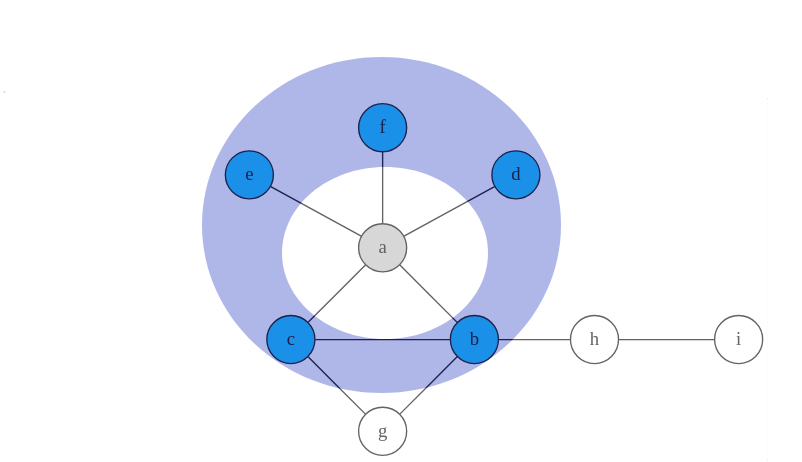
\includegraphics[width=0.5\textwidth]{MB_graph_shaded}
	\caption{The blue nodes form a \textit{blanket} around node 'a', rendering it conditionally independent of the remaining network.}
	
	\label{fig:MB_shaded}
\end{figure}

%When assuming that the data follows a multivariate Gaussian distribution, 
%In the setting of Gaussian Graphical Models (i.e. the assumption of multivariate normally distributed data) conditional independencies between variables are indicated by zero-entries of the inverse covariance matrix, which is also known as the precision matrix.
%With this in mind, the problem can be reformulated to the estimation of the precision matrix.
%In classical statistics this problem is traditionally referred to as "Covariance Selection".
In statistics the general problem of inferring the dependence structure of (assumed) Gaussian distributed data is classically known as \textit{Covariance Selection} \cite[]{price1972extension}, because the zero-pattern of the inverse covariance matrix encodes conditional independencies. 
Since dependence structures can be conveniently expressed in the form of a network graph (see \autoref{fig:cov_to_GMM}), the problem now tends to be referred to as the estimation of a \gls{GGM}.
\begin{figure}
	\hspace*{2cm}
	$\text{sign}(\matr{\Sigma^{-1}})=$
	$\Bigg($
	\begin{tabular}{cccc}
		\textbf{a} & \textbf{b} & \textbf{c} & \textbf{h}\\
		1&1&1&0\\
		1&1&1&-1\\
		1&1&1&0\\
		0&-1&0&1\\
		&&&
	\end{tabular}%
	$\Bigg)$
	\begin{tabular}{l}
		\\
		\textbf{{a}} \\
		\textbf{{b}} \\
		\textbf{{c}} \\
		\textbf{{h}} \\
		\\
	\end{tabular}
	$\Huge\Rightarrow$
	\makebox[0pt][l]{\raisebox{-10ex}{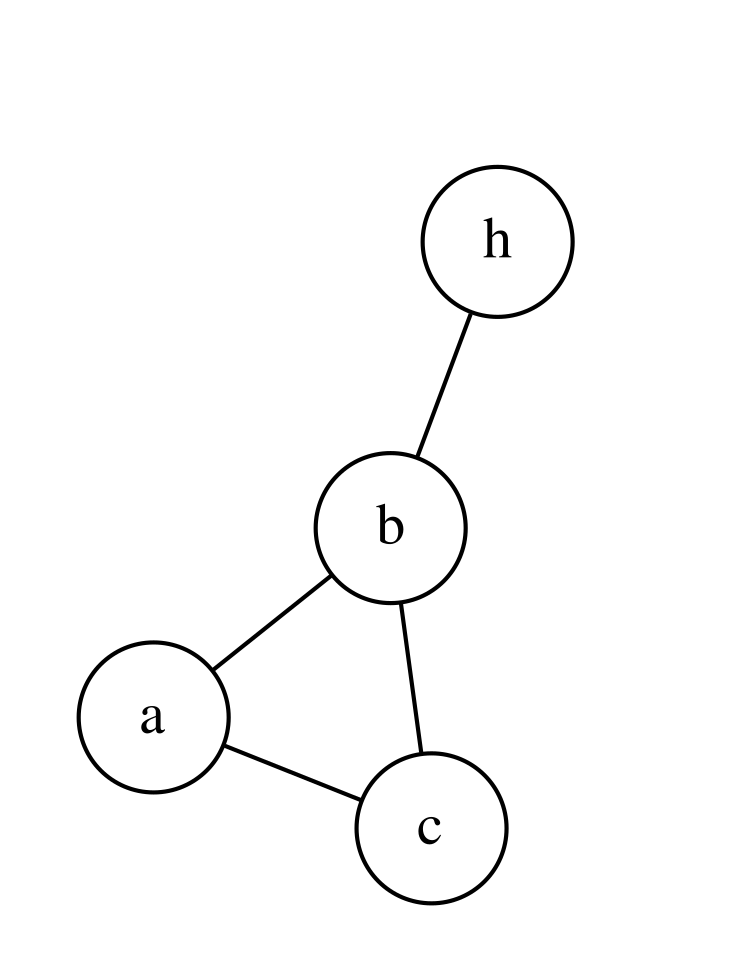
\includegraphics[width=0.2\textwidth]{MB_graph_small.png}}}%
\caption{Example for a dependency network encoded by the zero-pattern of the inverse covariance matrix.}
\label{fig:cov_to_GMM}
\end{figure}

Many popular approaches for estimating such \gls{GGM}s are based on enforcing sparsity in the network.
A sparse network is generally favorable for its interpretability, since large and densely connected graphs are difficult to analyze.
Prominent examples of sparse network estimation are the Graphical LASSO \cite[]{friedman_sparse_2008} and its Bayesian perspective \cite[]{wang_bayesian_2012}.
As with many alternative approaches, they infer the full network,
which is not always required for the problem at hand.
In many real-world problems there are often only a few variables of interest (e.g. clinical factors) which might interact with a great number of other variables (e.g. genetic markers).
The interactions between these few variables and the others are often the ones of highest interest.
In such cases inferring the whole network might be unnecessary and computationally expensive (especially for models that rely on simulation, such as \gls{MCMC} methods).
Consequently, it would be advantageous to limit estimation to the subnetwork of interest, and the \gls{BMB} estimation by \citet{kaufmann_bayesian_2015} offers such an approach.
By avoiding the inference of the whole network, the method allows for a more efficient estimation than related Bayesian methods (e.g. \citet{wang_bayesian_2012}) when the Markov Blanket of a few variables is of importance.
\citet{kaufmann_bayesian_2015} infer the whole posterior distribution.
However, in practice a point estimate is often desired, among others for the sake of interpretability and convenience.
While we could base this estimate on statistics such as the mean or median of the empirical posterior,
the most probable point, name the \gls{MAP}, would be more sensible in many cases.
However, estimating this mode from the empirical posterior distribution acquired by MCMC sampling poses some problems
in high dimensional settings.
The estimation would require some sort of binning or kernel density estimation,
which generally does not scale well for higher dimensions due to the 'curse of dimensionality' \citep{stone1980optimal, scott1991feasibility}.
Furthermore, if the mode is not surrounded by a lot of probability mass, the majority of the simulation time will be spent exploring regions of lower interest.
We address this issue by introducing \gls{SA} to the Bayesian Markov Blanket estimation, allowing for a direct and more robust estimation of the \gls{MAP}.
Because Simulated Annealing is seamlessly added on top of an already existing MCMC sampler,
small changes of the original model, such as the introduction of (hyper) priors, can be integrated into the MAP estimation.
Compared to the non-Bayesian approach, \gls{SA} also gives the advantage of having both the full posterior and a point estimate for the same model available, if it is desired.
Performance of the Annealing in comparison to the \gls{BMB} and the Graphical LASSO is evaluated on artificial data.
Furthermore, we investigate the modality of the posterior as well as the general behavior of the model
on both artificial and real data.

As already mentioned, learning dependencies inherent to the data can be very useful in medical domains.
In context of this thesis, we will focus on the area of HIV-1 treatment responses for individuals that
have been successfully treated for more than five years.
While current treatments are capable of suppressing the virus, it cannot be fully exterminated and dormant viral populations will multiply again after treatment stop. 
Furthermore, mutations of the virus might result in resistances that can affect current and future treatments.
We aim to find potential dependencies between resistance relevant mutations in latent viral populations and clinical factors that quantify the success of the treatments (e.g. the viral load and CD4 cell counts).
Additionally, dependencies between the clinical factors and the prior \& current treatment of the patients are of interest.
Discovering these dependencies might for example serve as a preliminary feature selection step for predicting the success of antiretroviral treatments for individual patients.
This serves as our motivation for estimating the Markov Blankets of the clinical factors.
The data used for this originates from the SystemsX.ch HIV-X project \citep{HIVX} and the Swiss HIV Cohort Study \citep{SHCS}.

The thesis is divided into 6 chapters.
After a short overview of existing related work, the general background required for the \gls{BMB} and \gls{SA} is given.
On top of a basic overview of used statistical tools, we elaborate on the need for enforcing sparsity in the process of network estimation. 
In the third chapter, the \gls{BMB} model itself as well as its extension are presented.
This is mostly limited to a theoretic overview.
Details regarding the implementation, as well as the setup for the artificially created data are discussed in the fourth chapter.
Subsequently, we present the results obtained from the application on both synthetic data and HIV.
Finally, a conclusion as well as an outlook for possible future work is given.

\section{Contributions}
With the general goals outlined, 
the contributions of this thesis can be summarized to the following points:
\begin{itemize}
	\item Introduction of Simulated Annealing to Bayesian Markov Blanket estimation \citep{kaufmann_bayesian_2015}
	\item Evaluation and Comparison of \gls{BMB}, \gls{SA} and the Graphical LASSO on artificial data
	\item Experimental study regarding the modality of the underlying model
	\item Analysis of potential dependencies in the SystemsX.ch HIV-X cohort data \citep{HIVX, SHCS} with Markov Blanket estimation
	
\end{itemize}
\chapter{Background and Related Work}
In the following chapter the background necessary for the Bayesian Markov Blanket Estimation and its extension with Simulated Annealing is provided.
First, the statistical methods used for the inference of our models are covered.
This includes \gls{MCMC} sampling for the estimation of the whole posterior distribution and Simulated Annealing for a \gls{MAP} estimate.
Subsequently, copulas and more specifically the semi parametric Gaussian copula are presented.
Copulas allows generalizing the \gls{BMB} and similar models to mixed data by introducing latent variables and relaxing the assumptions about the marginal distributions of the data.
At last we introduce Gaussian Graphical Models and the matters of their estimation in a high-dimensional setting.


\section{Markov Chain Monte Carlo}
This section is mainly based on \citet{andrieu2003introduction}, which provides an overview and introduction to \gls{MCMC} methods.

Bayesian inference allows us to update our prior beliefs when observing data to produce our posterior belief.
Let $\matr{\theta}$ be the parameters of a statistical model and $X$ the observed data distributed according to the (unknown) \gls{pdf} $p(X)$.
The Likelihood $p(X|\theta)$ then quantifies how 'likely' it is, that data $X$ was created according to the statistical model parametrized by $\theta$.
Preexisting and arguably subjective beliefs we have about the parameters are captured in the prior \gls{pdf} $p(\theta)$. 
When observing data $X$, the prior can then be updated to the posterior according to the well known Bayes' Theorem \cite[Chapter 1.2.3]{Bishop:2006:PRM:1162264}:
$$
p(\theta|X) = \frac{p(X|\theta) p(\theta)}{p(X)} =  \frac{p(X|\theta) p(\theta)}{\int_\Theta p(X|\theta')p(\theta') d\theta'}
$$
The posterior \gls{pdf} then expresses our uncertainty about $\theta$, while incorporating both the observed data and our prior beliefs.
Although the posterior can be given as a closed-form expression in special cases (e.g. by using conjugate priors), this is generally not the case.
The main difficulty arises from the unknown $p(X)$.
Although it can be calculated by marginalization, the integral usually offers no analytical solution, and numerical integration is computationally intractable for even moderately large parameter spaces.
For tackling this problem, \gls{MCMC} methods can be used.
MCMC techniques provide a framework for sampling from target distributions which can be evaluated up to a normalizing constant.
As such, the posterior distribution can be empirically estimated without the need to explicitly compute the prohibitively large normalization.

Because the posterior need be known only up to a constant, knowing the likelihood $p(X|\theta)$ and the prior $p(\theta)$ is sufficient:
$$
p(\theta|X) = \frac{p(X|\theta)p(\theta)}{\int_\Theta p(X|\theta')p(\theta') d\theta'} \propto p(X|\theta)p(\theta)
$$

Sampling from a target distribution is achieved by constructing homogeneous, 'irreducible and aperiodic Markov chains that have the target distribution as the invariant distribution' \citep{andrieu2003introduction}.
That is, the chain must not have any cycles (\textit{aperiodicity}) and every state with non-zero probability must be reachable within a finite number of steps (\textit{irreducibility}).
A sufficient (but not necessary) condition for having a specific distribution $p(x)$ as the invariant distribution of a discrete Markov chain with transition matrix $T$ is the \textit{detailed balance} property (\cite[Chapter 11.2.1]{Bishop:2006:PRM:1162264}):
\begin{equation}
	\label{eq:mcmc_invar}
	p(x^{(i)})T(x^{(i-1)} | x^{(i)})=  p(x^{(i-1)})T(x^{(i)} | x^{(i-1)})
\end{equation}
By constructing a Markov chain that satisfies these conditions, a corresponding sampler can then be constructed.
The empirical distribution of the samples drawn from the chain then converges \textit{almost surely} to the target distribution, which in our case is the posterior distribution.
But while convergence itself might be a.s. guaranteed for $n\rightarrow \infty$, the convergence rate
strongly depends on the specific Markov chain used. So while fulfilling the necessary conditions might be sufficient in theory, a Markov chain with quick convergence is required in practice.
In the following subsections we will present two well known MCMC techniques for sampling from a target distribution.
 
\subsection{Metropolis Hastings}
Metropolis Hastings (MH) is a \gls{MCMC} method introduced by \citet{hastings1970monte}.
While we do not directly make use of a \gls{MH} sampler in the presented models, \gls{MH} can be viewed as a general case of other samplers. 
As we'll show in the following sections, this will be useful for extending a Gibbs Sampler for Simulated Annealing.

The \gls{MH} procedure is based on drawing samples from a proposal function and then randomly accepting or rejecting them as draws from the target distribution.
Let $p(x)$ be the invariant distribution we are interested in (known up to a constant) and $q(x^*|x)$ some proposal function. The proposal function suggests a new candidate for our sampler, given a current value.
Unlike the Metropolis sampler \citep{metropolis1953equation}, \gls{MH} does not require the proposals to be symmetric.
\begin{algorithm}[H]
	\caption{Metropolis-Hastings Sampler}\label{alg:MH}
	\begin{algorithmic}
		\State \textbf{Initialize}: $x^{(0)}$
		\For{$i=0$ to $N-1$}
		\State Sample $u\sim \mathcal{U}_{[0,1]}$
		\State Sample $x^* \sim q(x^*|x^{(i)})$
		\If{$u< \mathcal{A}(x^{(i)}, x^*) = 
			\min 
			\Big\{ 
			1, \frac{p(x^*)q(x^{(i)} | x^*)}
			{p(x^{(i)})q(x^*|x^{(i)})} 
			\Big\} $}
		\State $x^{(i+1)} = x^*$
		\Else
		\State $x^{(i+1)} = x^{(i)}$
		\EndIf
		\EndFor
	\end{algorithmic}
\end{algorithm}

In Algorithm \autoref{alg:MH} the general sampler for which the Markov chain admits $p(x)$ as the invariant distribution is shown.
By construction, the transition probabilities of the \gls{MH} sampler satisfy \autoref{eq:mcmc_invar}. 
The aperiodicity of the chain is given by the possibility of rejection in the sampler.
For guaranteeing irreducibility, it need only be ensured that the proposal function $q(x*|x)$ has the same support as $p(x)$ (i.e. can lead to all states $x^*$ that have non-zero probability $p(x^*)$).
It should be noted, that $p(x)$ need be known only up to a constant. 
This follows from the fraction $\frac{p(x^*)q(x^{(i)} | x^*)}
{p(x^{(i)})q(x^*|x^{(i)})} $ which is not affected by a constant factor in $p(x)$.
While \gls{MH} is a very general method, its performance largely depends on the proposal function.
If the proposals are too conservative (i.e. if there are only very small changes compared to the previous sample), exploring the whole posterior will take a long time.
Conversely a proposal function that jumps around a lot may suffer from a low acceptance ratio, as many improbable values are considered.


\subsection{Gibbs Sampling}
\label{ss:Gibbs}
Gibbs sampling \citep{geman1984stochastic} is an MCMC method that can be applied if the target distribution is multivariate.
Instead of the joint distribution, it relies on the individual conditional distributions and is especially useful if the conditionals are known and easy to sample from.

Let $p(\matr{x}) = p(x_1, \dots, x_n)$ be the distribution we wish to sample from,
where the conditionals $$p(x_j|x_{-j}) = p(x_j | x_1, \dots x_{j-1}, x_{j+1}, \dots, x_n) \quad \quad \forall j \in \{1,\dots,n\}$$ are known.
By now iteratively drawing samples from the individual distributions while conditioning on the latest drawn samples of the other parameters, we can approximate the joint posterior $p(x_1,\dots,x_n)$.
This is convenient since the posterior conditionals can often be expressed in terms of a known closed form distribution (by using semi-conjugate priors), even if the full posterior cannot.

The Gibbs sampler can be viewed as a special case of Metropolis Hastings with the following distribution for the proposal function \citep{andrieu2003introduction}:
$$
q(x^*|x^{(i)}) = 
\left\{
\begin{array}{ll}
	p(x^*_j|x^{(i)}_{-j}) & \text{If } x^*_{-j} = x^{(i)}_{-j} 
	\\
	0                     & \text{otherwise}                   
\end{array}
\right.
$$

Substituting this into Algorithm \autoref{alg:MH} and using $p(x) = p(x_j|x_{-j}) p(x_{-j})$
leads to \cite[p. 544]{Bishop:2006:PRM:1162264}
$$
\mathcal{A}(x^{(i)}, x^*) = 
\min 
\Big\{ 
1, \frac{ p(x^*_j|x^*_{-j}) p(x^*_{-j}) p(x_j|x^*_{-j})}
{  p(x_j|x_{-j}) p(x_{-j}) p(x^*_j | x_{-j})  } 
\Big\} 
= 1
$$
Thus, the Gibbs sampler is a \gls{MH} sampler with acceptance probability $1$.
This perspective can now be used for incorporating Simulated Annealing on top of a Gibbs sampler, for which the posterior conditionals are available in closed forms.

The general sampler is shown in Algorithm \autoref{alg:Gibbs}.
Each iteration of it corresponds to a Gibbs sweep, where a new sample is drawn for each variable while conditioning on the most recent samples of the other variables.
Thus,  one draw from the joint distribution is obtained with each Gibbs sweep.
It should be noted, that the order of the variables does not influence the sample distribution for a sufficiently large number of iterations.
\begin{algorithm}[H]
	\caption{Gibbs Sampler}\label{alg:Gibbs}
	\begin{algorithmic}
		\State \textbf{Initialize}: $x_{0, 1:n}$
		\For{$i=0$ to $N-1$}
		\State Sample $x_1^{(i+1)}\sim p(x_1|x_2^{(i)}, x_3^{(i)}, \dots, x_n^{(i)})  $
		\State Sample $x_2^{(i+1)}\sim p(x_2|x_1^{(i+1)}, x_3^{(i)}, \dots, x_n^{(i)})  $
		\\
		\State \vdots
		\\
		\State Sample $x_j^{(i+1)}\sim p(x_j|x_1^{(i+1)}, x_{j-1}^{(i+1)},x_{j+1}^{(i)}, \dots, x_n^{(i)})  $
		\\
		\State \vdots
		\\
		\State Sample $x_n^{(i+1)}\sim p(x_n|x_1^{(i+1)}, x_2^{(i+1)}, \dots, x_{n-1}^{(i+1)})  $
		\EndFor
	\end{algorithmic}
\end{algorithm}

\FloatBarrier


\subsection{Simulated Annealing}
\label{ss:SA}
If we are only interested in a point estimation of the parameters, 
inferring the whole posterior distribution might not be the best solution.
Unless the area surrounding the mode of the posterior has a high amount of probability mass, the sampler will mainly explore areas that are of low interest.
Instead we can try to directly find the mode of the posterior, i.e. the \gls{MAP}.
Simulated Annealing \citep{kirkpatrick1983optimization} is an optimization framework that can be used for finding the global maximum of a given function.
The concept stems from metallurgy, where slowly cooling a previously heated material leads to it reaching an 'optimal' minimum energy state.


For applying \gls{SA} in the context of \gls{MCMC} sampling, we switch to a inhomogeneous Markov chain with the invariant distribution
$$ p_i (x) \propto p^{1/T_i} $$
where $T_i$ is the temperature at iteration $i$. 

Initially the temperature is very high, such that large jumps between the drawn samples are possible (as the invariant distribution will be very flat). 
The temperature is then slowly decreased, such that the distribution becomes more peaked and less jumping is possible. 
Eventually the invariant $p^{1/T_i}(x)$ tends to $p^\infty(x)$ for $lim_{i\rightarrow \infty}T_i=0$, which concentrates on the global maxima.
The concrete value of $T_i$ and its speed of decrease are defined by a cooling schedule $f_T(i)$. 
Convergence to the set of global maxima has been shown to hold for logarithmic cooling schedules in discrete domains \citep{geman1984stochastic}.
Unfortunately, a logarithmic cooling schedule is not a computationally feasible option for realistic problem sizes.
In the literature, a range of cooling schedules has been analyzed (e.g. \citet{abramson1999simulated}), but to our knowledge there is not one distinct cooling method that works best in practice.
In general, slower cooling of the system is preferred and the decrease in temperature should slow down with the temperature going towards 0.
A simple method that is quite popular in practice is a geometric cooling schedule
(see for example \cite{andrieu2000simulated, yuan2004annealed}).

\begin{tcolorbox}[title=Geometric Cooling Schedule (1)]
	Let $T_0$ be the initial temperature, $a\in\mathbb{R}_{> 0}$ be a constant.
	Then the temperature $T_i$ at iteration $i$ is:
	$$
	T_i = f_T(i) = T_0\  a^{i} \quad \quad i = 0,1,\dots,n
	$$
\end{tcolorbox}

Furthermore, as $\frac{1}{T}$ can never reach infinity in practice, one can set a (low) target temperature $T_n$, which is reached after $n$ iterations.
Adapting the geometric cooling schedule to reach a final temperature $T_n$ leads to:
\begin{tcolorbox}[title=Geometric Cooling Schedule (2)]
	\begin{equation}
		f_T(i) = T_0  \Big(\frac{T_n}{T_0}\Big)^{i/n} \quad \quad i = 0,1,\dots,n
	\end{equation}
\end{tcolorbox}
The form of the geometric cooling schedule can be seen in \autoref{fig:cool_exp}.
\begin{figure}
	\centering
	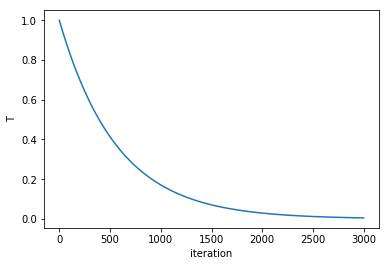
\includegraphics[width=0.5\textwidth]{cool_exp}
	\caption{Geometric cooling schedule for $T_n=0.005$, $T_0=1$ and $n=3000$}
		
	\label{fig:cool_exp}
\end{figure}

At the target temperature we can continue sampling from the invariant distribution $p^{1/T_n}(x)$. 
If convergence was achieved (i.e. if the cooling was slow enough) samples from this target temperature will be close to the true mode with high probability.
For estimating the final value, we can then for example look at statistics such as the median, mean or the credible intervals of the samples.
The Annealing can be implemented by slightly altering the \gls{MH} sampler, such that the invariant distribution at each step is $p^{1/T_i}(x)$, where the temperature $T_i$ is set according to the cooling schedule $f_T(i)$ (see Algorithm \autoref{alg:SA_MH}).


\begin{algorithm}[H]
	\caption{Simulated Annealing: Metropolis-Hastings}\label{alg:SA_MH}
	\begin{algorithmic}
		\State \textbf{Initialize}: $x^{(0)}$, $T_0=1$
		\For{$i=0$ to $N-1$}
				
		\State $T_{i} = f_T(i)$
		\\
		\State Sample $u\sim \mathcal{U}_{[0,1]}$
		\State Sample $x^* \sim q(x^*|x^{(i)})$
		\If{$u< \mathcal{A}(x^{(i)}, x^*) = 
			\min 
			\Big\{ 
			1, \frac{p(x^*)^{1/T_i} q(x^{(i)} | x^*)}
			{p(x^{(i)})^{1/T_i}q(x^*|x^{(i)})} 
			\Big\} $}
		\State $x^{(i+1)} = x^*$
		\Else
		\State $x^{(i+1)} = x^{(i)}$
		\EndIf
		\EndFor
	\end{algorithmic}
\end{algorithm}
Similar to \autoref{ss:Gibbs}, it is possible to use the conditional distributions as proposals:
$$
q(x^*|x^{(i)}) = 
\left\{
\begin{array}{ll}
	p(x^*_j|x^{(i)}_{-j})^{1/T_i} & \text{If } x^*_{-j} = x^{(i)}_{-j} 
	\\
	0                             & \text{otherwise}                   
\end{array}
\right.
$$
As before, one can show that this leads to an acceptance probability of 1 when input into Algorithm \autoref{alg:SA_MH}.
In consequence we can formulate the Simulated Annealing for a Gibbs sampler as shown in Algorithm \autoref{alg:SA_Gibbs}.

\begin{algorithm}[H]
	\caption{Simulated Annealing: Gibbs Sampler}\label{alg:SA_Gibbs}
	\begin{algorithmic}
		\State \textbf{Initialize}: $x_{0, 1:n}$, $T_0=1$
		\For{$i=0$ to $N-1$}
		\State $T_{i} = f_T(i)$
		\\
		\State Sample $x_1^{(i+1)}\sim p(x_1|x_2^{(i)}, x_3^{(i)}, \dots, x_n^{(i)})^{1/T_i}  $
		\State Sample $x_2^{(i+1)}\sim p(x_2|x_1^{(i+1)}, x_3^{(i)}, \dots, x_n^{(i)})^{1/T_i}  $
		\\
		\State \vdots
		\\
		\State Sample $x_j^{(i+1)}\sim p(x_j|x_1^{(i+1)}, x_{j-1}^{(i+1)},x_{j+1}^{(i)}, \dots, x_n^{(i)})^{1/T_i}  $
		\\
		\State \vdots
		\\
		\State Sample $x_n^{(i+1)}\sim p(x_n|x_1^{(i+1)}, x_2^{(i+1)}, \dots, x_{n-1}^{(i+1)})^{1/T_i} $
		\EndFor
	\end{algorithmic}
\end{algorithm}

\section{Semi-Parametric Gaussian Copula}
\label{s:semi_copula}
In many problem settings it is common to have mixed data for which we cannot assume a specific (closed form) marginal distributions,
while we still would like to assume a joint distribution of the data.
However, a model that would for example be based on multivariate Gaussian data also relies on univariate Gaussian marginals.
A solution for this is provided by Sklar's theorem \citep{sklar1959fonctions}, which says that a $p$-dimensional joint distribution can be represented in two parts: The $p$ marginal distributions and a \textit{copula} function, which describes the dependencies between the variables.
\begin{tcolorbox}[colback=yellow!5!white,colframe=yellow!75!black, title=Sklar's Theorem]
	\begin{customthm}{}[extracted from \citet{nadarajah2018compendium}]
		\label{th:sklar}
		Let \textit{F} be a \textit{p}-dimensional cumulative distribution function with marginal distribution functions $F_i, i=1,\dots,p$. Then there exists a copula C such that
		$$
		F(x_1,\dots,x_p) = C(F_1(x_1), \dots, F_p(x_p))
		$$
		Conversely, for any univariate cumulative distribution functions 
		$F_1,\dots, F_p$
		and any copula $C$, the function $F$ is a $p$-dimensional \gls{cdf} with marginals $F_1,\dots,F_p$. 
		Furthermore, if $F_1, \dots, F_p$are continuous, then C is unique.
	\end{customthm}
\end{tcolorbox}
So with the use of copulas, it is possible to parametrize the marginal distributions separately from their joint distribution. 
Consequently the dependency structure of the data can be assumed to follow a specific joint distribution (e.g. a multivariate Gaussian) without having to consider the unknown marginals.
It should be noted that Sklar's Theorem guarantees the uniqueness of the copula only where marginals are continuous.

Let $y_{i,j}$ be the $i$-th observation of variable $\matr{y}_j$, with $i=1,\dots,n$ and $j=1,\dots,p$.
For modeling the copula, latent variables $\matr{z}_j$ that are distributed according to the assumed joint distribution are introduced. 
The observed variables $y_{i,j}$ can then be represented as the result of a non-decreasing transformation $g_j(z_{i,j})$ of the latent data.
In the case of Gaussian copula models we assume that the latent variables are distributed according to a multivariate Normal distribution and can be modeled as follows
\citep{hoff2009first}.
\begin{tcolorbox}[colback=yellow!5!white,colframe=yellow!75!black, title=Gaussian Copula: Latent Normal Model]
	Let $\matr{z}_1, \dots, \matr{z}_n$ be $i.i.d.$ (latent) random variables drawn from a p-variate normal distribution, with $\matr{C}$ being a $p\times p$ correlation matrix.
	Furthermore, let $\matr{y}_j$ be the observed variables with marginal \gls{cdf} $F_j$. 
	With $g_1,\dots,g_p$ being non-decreasing functions, the Gaussian copula model is
	\begin{equation}
		\label{eq:gauss_copula}
		\matr{z}_1, \dots, \matr{z}_n | \matr{C} \overset{i.i.d.}{\sim}  N(0, \matr{C})
	\end{equation}
	$$
	y_{i,j} = g_j(z_{i,j}) = F_j^{-1}(\Phi(z_{i,j}))
	$$
\end{tcolorbox}
The aim now is to estimate $\matr{C}$, as we are interested in the interactions of the data. 
If the marginal distributions are known and continuous, the computation is trivial. 
The $z_{i,j}$ could be directly computed from the observed values. 
Inference of $C$ could then be done by using standard estimation methods suitable for Gaussian data.

While many approaches do use parametric distributions for modeling the marginals,
\citet{2007extending} introduce a semi-parametric Gaussian copula estimation dealing with both unknown and discrete marginals.
It is semi-parametric in the sense that the model still parametrizes the joint \gls{pdf} as a multivariate Gaussian, but does not make any assumptions about the marginals.
This is achieved by basing the estimation of $\matr{C}$ on an 'extended rank likelihood', which is based only on an order preserving statistic of the observations $y_{i,j}$, independent of the marginals $F_j$.


\subsection{The extended rank likelihood}
As it is given that the $F_j$s are non-decreasing, the order of the observations of $\matr{y}_j$ will always be preserved for any transformation by $F_j$.

Let 
$\matr{Z} = (\matr{z}_1, \dots, \matr{z}_n)^T$ and $\matr{Y} = (\matr{y}_1, \dots, \matr{y}_n)^T$
then $\matr{Z}$ must lie in the set
\begin{equation}
	\label{ext_rankl_set}
	\{\matr{Z}\in \mathbb{R}^{n\times p} : max\{z_{k,j}:y_{k,j}<y_{i,j}\} <z_{i,j} <min\{z_{k,j}:y_{i,j}<y_{k,j}\}  \} 
\end{equation}
So the latent value $z_{i,j}$ for an observation $y_{i,j}$ is always constricted 
by the latent values corresponding to the two neighboring observations $max\{y_{k,j}:y_{k,j}<y_{i,j}\}$  and $min\{y_{k,j}:y_{i,j}<y_{k,j}\}$.
\autoref{table:rankll} provides a visualization for this relationship.
\\
\\
\begin{figure}[H]
	\begin{tcolorbox}[colback=green!5!white,colframe=green!75!black]
		\begin{tabular}{cccccc}
			&\multicolumn{5}{c}{$\xrightarrow{\hspace*{7cm}}$}
			\\
			$\matr{y}\quad\quad$ & $max(y_{k,j}:y_{k,j}<y_{i,j})$   & $<$           & $y_{i,j}$                 & $<$         & $min(y_{k,j}: y_{k,j}>y_{i,j})$ 
			\\
			                     &                                  &               &                           &             &                                 
			\\
			\midrule
			                     &                                  & $\downarrow $ & \quad\quad\quad\quad\quad & $\uparrow$  &                                 
			\\
			                     &                                  & $ F_j^{-1}$   & \quad\quad\quad\quad\quad & $ F_j$      &                                 
			\\
			                     &                                  & $\downarrow $ & \quad\quad\quad\quad\quad & $\uparrow $ &                                 
			\\
			\midrule
			                     &                                  &               &                           &             &                                 
			\\
			$\matr{z}\quad\quad$ & $max\{z_{k,j}:y_{k,j}<y_{i,j}\}$ & $<$           & $z_{i,j}$                 & $<$         & $min(z_{k,j}: y_{k,j}>y_{i,j})$ 
		\end{tabular}	
				
	\end{tcolorbox}
	\caption{Relationship between latent values and observations.}
	\label{table:rankll}
\end{figure}



Since $\matr{Z}$ always lies in this set for any observed $\matr{Y}$,
we can write the likelihood as:
\begin{align*}
	p(\matr{Y}|\matr{C}, F_1, \dots, F_p) & = p(\matr{Z}\in D, \matr{Y}|\matr{C}, F_1, \dots, F_p) 
	\\
	                                      & =                                                      
	p(\matr{Z}\in D|\matr{C}, F_1, \dots, F_p)
	p(\matr{Y}|\matr{Z}\in D, \matr{C}, F_1, \dots, F_p)
	\nonumber
\end{align*}

As  $\{\matr{Z} \in D\}$ is independent of  $F_j$ due to the order preservation, it follows that
\begin{equation}
	\label{ext_rankl}
	P(\matr{Z}\in D|\matr{C}, F_1, \dots, F_p) = P(\matr{Z}\in D| \matr{C})
\end{equation}
\autoref{ext_rankl} is then called the 'extended rank likelihood'.
Using this likelihood, a Gibbs sampler for the posterior 
\begin{equation}
	\label{eq:posterior_copula}
	p(\matr{C}|\matr{Z}\in D)\propto p(\matr{C})\times p(\matr{Z}\in D | \matr{C})
\end{equation}
can be constructed by choosing a semi-conjugate prior for $\matr{C}$.

\subsection{Gibbs Sampler}
Because of our model's assumption of a joint normal distribution in  \autoref{eq:gauss_copula}, and the constriction due to the extended rank likelihood by \autoref{ext_rankl_set}, the conditional posteriors of $z_{i,j}$ follow a truncated normal distribution.
Furthermore we can base the inference on the covariance matrix $\matr{V}$ instead of the correlation matrix $\matr{C}$ for easing the construction of a sampler.
As the correlation matrix $\matr{C}$ can be calculated from $\matr{V}$, we will get an equivalent model.
For the prior $p(\matr{V})$ an inverse Wishart prior with expected value $E[\matr{V}^{-1}] = \matr{V}_{0}^{-1}$  is suggested by \citet{2007extending}.

This results in the model
\begin{align*}
	V \sim                                            & \ \mathcal{W}^{-1}(v_0, v_0\matr{V}_0)                         
	\\
	\matr{C} =                                        & \ \text{diag}(V)^{-\frac{1}{2}}V \text{diag}(V)^{-\frac{1}{2}} 
	\\
	\matr{z}_1\dots,\matr{z}_n \overset{i.i.d.}{\sim} & \  \mathcal{N}(\matr{0}, \matr{C})                             
	\\
	\tilde{z}_{i,j} =                                 & \  z_{i,j} / \sqrt{\matr{V}_{j,j}}                             
	\\
	y_{i,j} =                                         & \ F_j^{-1}(\tilde{z}_{i,j})                                    
\end{align*}

with posterior conditionals

\begin{align*}
	z_{i,j}|(\matr{V}, \matr{Z}_{-i,-j}, \matr{Z}\in D)  
	\sim &                                                                                                 
	\mathcal{TN}
	(\mu_{i,j}, \sigma_j, a_j, b_j)
	\\
	     & \quad\mu_{i,j}=\matr{Z}_{i,-j}\Big(\matr{V}_{j,-j} \matr{V}_{-j,-j}^{-1} \matr{V}_{-j,j}\Big)^T 
	\\
	     & \quad\sigma_j^2 = \matr{V}_{j,j} - \matr{V}_{j,-j}\matr{V}_{-j,-j}^{-1}\matr{V}_{-j,j}          
	\\
	     & \quad a_j = \sup(z_{k,j} : y_{k,j}<y_{i,j})                                                     
	\\
	     & \quad b_j = \inf(z_{k,j} : y_{i,j}<y_{k,j})                                                     
	\\
	\matr{V}|(\matr{Z}\in D) 
	\sim &                                                                                                 
	\mathcal{W}^{-1}(v_0+n, v_0\matr{V}_0+ \matr{Z}^T\matr{Z})
\end{align*}
It should be noted that there are no bounds for missing values $y_{i,j}$ 
and the latent values $z_{i,j}$ are then imputed by using the (non-truncated) Gaussian distribution.
In the present context we use a more efficient formulation suggested by \citet{adametz2014information}.
It avoids matrix inversions in the inner-most loop by using a Wishart prior for sampling from the inverse covariance matrix, instead of an inverse Wishart prior for the covariance matrix.
Furthermore, $\matr{Z}$ is initialized with its normal scores (see \citet{rey2012meta}):
$${z}_{i,j} = \Phi^{-1}\Big(\frac{\text{rank}_j(y_{i,j})}{n_j+1} \Big)$$
where $n_j$ denotes the number of levels of variable $j$, i.e. the number of unique observed values of $\matr{y}_j$.
In the following chapters it will be clear that this formulation works well in our context due to each of the \gls{BMB}s Gibbs sweeps effectively being a draw from the precision matrix.
The full sampler of this formulation for the semi-parametric copula is shown in Algorithm \autoref{alg:copula}. 

\begin{algorithm}[]
	\caption{Gibbs Sampler: Semi-Parametric Gaussian Copula}\label{alg:copula}
	\begin{algorithmic}
		\State \textbf{Input}: $n \times (p+q)$ data matrix $\matr{Y}$ containing observations from $p+q$ rvs
		\State \textbf{Set}:
		$V \gets I_{p+q}$, 
		$V_0 \gets I_{p+q}$, 
		$v \gets (p+q+1)$
		\State \textbf{Initialize}:
		${{Z}} = 
		\Big\{
		{z}_{i,j} \gets \Phi^{-1}
		\Big(\frac{\text{rank}_i(y_{i,j})}{n_i+1} \Big)$ for $j\in \{1,\dots,(p+q)\}, i \in \{1,\dots,n\}$
		\Big\}
		%\For{$k = 1,\dots,N_{GibbsSamples}$}
		\Repeat
		\For{$j = 1,\dots,(p+q)$}
		\State $\sigma^2_j \gets 1/V_{j,j}$
		\For{$y \in unique\{y_{1,j}, \dots, y_{n,j}\}$}
		\State Find lower bound $a \gets \sup(z_{i,j} : y_{i,j} < y)$
		\State Find upper bound $b \gets \inf(z_{i,j} : y<y_{i,j})$
		\For{each $i$ such that $y_{i,j}=y$}
		\State $\mu_{i,j} \gets -\sigma_j^2 z_{i,-j}V_{-j,j}$
		\State Sample $z_{i,j} \sim \mathcal{TN}(\mu_{i,j}, \sigma_j^2, a, b)$
		\EndFor
		\EndFor
		\EndFor
		\State Sample $V\sim \mathcal{W}_{p+q}(v+n, [V_0 + Z^T Z]^{-1})$
		\State Compute $\matr{C} = \Big\{ 
		\matr{C}_{i,j}\gets (V^{-1}_{i,j} / \sqrt{(V^{-1})_{u,u} (V^{-1})_{j,j}})
		\text{ for } (i,j) \in \{1,\dots,(p+q)\}
		\Big\}$
		\State Compute $\tilde{Z} = \Big\{ 
		\tilde{z}_{i,j} \gets z_{i,j} / \sqrt{(V^{-1})_{j,j}}$
		for $j\in \{1,\dots,(p+q)\}, i \in \{1,\dots,n\}\Big\}$
		%\EndFor
		\Until{converged}
	\end{algorithmic}
\end{algorithm}

\FloatBarrier


\section{Graphical Models}
\label{section:graphmodels}
Undirected Graphical Models provide a convenient framework for representing dependencies between random variables in the form of network graphs.
In the literature they are also commonly referred to as Markov Random Fields. 
Let a graph $G = (V,E)$ be denoted by a set of nodes $V$ and a set of edges $E$.
Each node $v\in V$ then corresponds to a random variable $X_v$ and each edge connects two nodes.
Additionally, the graph fulfills the following properties \cite[Chapter 19.2]{Murphy2013Machine}:
\begin{itemize}
	\item \textbf{Global Markov property} Iff node v separates nodes s and t in the graph, s and t are conditionally independent given v:
	      $$v_A \bigCI v_B | v_C$$ 
	\item \textbf{Local Markov property} A node $v$ is conditionally independent of the remaining network given its immediate neighbors $N(v)$: 
	      $$v \bigCI V\setminus(N(v)\cup v) | N(v)$$
	\item \textbf{Pairwise Markov property} Two nodes $v$ and $t$ are conditionally independent given the remaining network if there is no direct edge between them:
	      $$v\bigCI t|V\setminus{s,t}$$
\end{itemize}

In general the graph structure is unknown and we wish to estimate it from observed data.
That is, we want to learn the dependencies inherent to the data.
The following section provides a short introduction to Gaussian Graphical Models and highlights some of the difficulties that arise when estimating them from high-dimensional data.

\subsection{Gaussian Graphical Models}
This chapter mainly follows Chapter 9.2 \& 9.3 of \citet{hastie2015statistical}.
\label{GRAPH_SELECTION}
In the setting of \gls{GGM}s, it is assumed that the $p$-dimensional data follows a Normal distribution:

\begin{equation}
	\label{eq:normal_dist}
	\matr{X} \sim \mathcal{N}_{p}(\boldsymbol{\mu}, \matr{\Sigma})
	\quad \quad
	\boldsymbol{\mu }\in \mathbb{R}^{p} \quad \matr{\Sigma}\in \mathbb{R}^{p\times p} 
\end{equation}
$$ P(\matr{x})_{\boldsymbol{\mu}, \matr{\Sigma}} = \frac{1}{(2\pi)^{p/2}\det(\matr{\Sigma})^{1/2}} \exp\Big(-\frac{1}{2}(\matr{x}-\boldsymbol{\mu})^T \matr{\Sigma}^{-1}(\matr{x}-\boldsymbol{\mu})\Big)$$

Alternatively the Gaussian can be represented in terms of the canonical parameters $\W\in \mathbb{R}^{p\times p}$ and  $\boldsymbol{\gamma} \in \mathbb{R}^p$, where $\matr{W} = \matr{\Sigma}^{-1}$
is the precision matrix:

$$ P(\matr{x})_{\boldsymbol{\gamma}, \matr{W}} = \exp \Big( 
\sum_{s=1}^{p}\lambda_s {x}_s - \frac{1}{2} \sum_{s,t=1}^{p} w_{st}{x}_s {x}_t + \frac{1}{2} \log\det[\matr{W}/(2\pi)]
\Big)$$
 
In this formulation the \gls{pdf} factorizes according to the zero entries of $\matr{W}$.
That is, if and exactly if (\textit{iff}) $w_{st}=0$ then $x_s$ and $x_t$ are conditionally independent of each other.
Therefore the zero pattern of the precision matrix encodes the conditional independencies of our model.
Combining this with the Markov properties of a graphical Model, a Graph can be constructed by connecting all pairs of nodes with non-zero entries in the precision matrix.
Aside from the conditional independencies, a measure of dependence between the variables is of importance.
It was shown by \cite{lauritzen1996graphical} that the partial correlation between two variables given all the other variables can be written in terms of the precision matrix.
\begin{tcolorbox}[colback=yellow!5!white,colframe=yellow!75!black, title=Partial Correlation Coefficient]
	Let $\matr{X}=(X^{(1)},\dots, X^{(p)})$ be Normal distributed with
	$$\matr{X}\sim \mathcal{N}_p(\boldsymbol{\mu}, \W^{-1})$$
	and let $V = \{1,\dots,p\}$.
		
	Then the partial correlation coefficient $\rho_{i,j}$ between $X^{(i)}$ and $X^{(j)}$, given all the other variables is
	\begin{equation}
		\rho_{i,j|V\setminus \{i,j\}} = - \frac{\W_{i,j}}{\sqrt{\W_{i,i}\W_{j,j}}}
		\qquad i\neq j
	\end{equation}	
		
	\citep{lauritzen1996graphical}
\end{tcolorbox}


With this relationship established, it is clear that estimating the structure of a \gls{GGM} is equivalent to finding precision matrix.
This problem is also commonly known in classical statistics, namely as covariance selection (see for example \citet{dempster1972covariance}).

\subsubsection*{Estimation}
By going back to \autoref{eq:normal_dist} the model can be further simplified.
As the interest lies only in the dependency structure, $\matr{\mu} = \matr{0}$ (i.e. mean-free data) is assumed.
The log likelihood of the observed data $X=(\matr{x}_1, \dots, \matr{x}_n)^T$ with $\matr{x}_i \in\mathbb{R}^{n}$ is then:

\begin{align*}
	\mathcal{L}(\matr{W}; X) & = \log\Bigg( 
	\prod_{i=1}^{n}
	(2\pi)^{-p/2} \det(\matr{W})^{1/2} \exp\Big(
	-\frac{1}{2} \matr{x}_i^T \matr{W} \matr{x}_i
	\Big)
	\Bigg)
	\\
	                         & =            
	\log\Bigg(
	(2\pi)^{-np/2} 
	\det(\matr{W})^{n/2} 
	\exp\Big(
	-\frac{1}{2} \sum_{i=1}^{n}\matr{x}_i^T \matr{W} \matr{x}_i
	\Big)
	\Bigg)
	\\
	                         & \propto      
	\frac{n}{2}\log\det(\matr{W})
	-\frac{1}{2} \sum_{i=1}^{n}\matr{x}_i^T \matr{W} \matr{x}_i
	\\
	                         & =            
	\frac{n}{2}\log\det(\matr{W})
	-\frac{1}{2} 
	\tr\Big(
	\sum_{i=1}^{n} \matr{x}_i \matr{x}_i^T \matr{W}
	\Big)
	\\
	                         & \propto      
	\log\det(\matr{W})
	-\tr\Big(
	\matr{S} \matr{W}
	\Big)
	\quad\quad\quad\quad\quad\quad
	\matr{S}= 	\frac{ 1}{n}\sum_{i=1}^{n} \matr{x}_i \matr{x}_i^T
\end{align*}

A simple and straightforward approach for estimating $\bm{W}$ would be (unregularized) \gls{MLE}. As it turns out, the \gls{MLE} is

$$
\matr{\hat{W}}_{MLE} = \arg\max\{
\log\det (\matr{W}) - \tr({\matr{S}\matr{W}})
\}
= \matr{S}^{-1}
$$


Although this MLE indeed converges to the true precision matrix as $n$ goes towards infinity, it fails to exist for high dimensional data \citep[Chapter 9.3.1]{hastie2015statistical}. 
The cause for this is the rank-degeneracy of the sample covariance for $p>n$.
This can be problematic for real world applications in the aforementioned areas, where very high dimensional data $(p\gg n)$ is common.
Furthermore we might want to estimate a \gls{GGM} that is interpretable (i.e. a GMM corresponding to a network with few edges).
This leads to the notion of estimating a sparse $\matr{W}$, as regularizing the likelihood would deal with both of these problems.
For enforcing a sparse solution, a $L_0$ penalty (i.e. a penalty based on the number of non-zero edges) would seem to be a logical choice.
But due to the highly non-convex nature of $L_0$, an approximation with the $L_1$ constraint is often preferred:

\begin{equation}
	\matr{W} = \arg \max \{ \log \det(\matr{W}) - \tr(\matr{SW}) - \rho ||\matr{W}||_1 \}
\end{equation}
This convex problem can be solved by various methods.
A popular approach is the "Graphical Lasso" \citep{friedman_sparse_2008} which solves
it by using a first-order block wise coordinate descent.
We will not go into further details of this approach, as we are interested in the Bayesian perspective of the problem.

\subsection{Bayesian Graphical Lasso}
\label{BGLASSO}
It is well known that an L1 penalized maximum likelihood estimation is equivalent to a \gls{MAP} with a double exponential prior \citep{tibshirani1996regression}.
The aforementioned GLASSO estimator can therefore be seen as equivalent to a maximum posterior estimation with a double exponential prior on the non-diagonal entries of $\matr{W}$.
Depending on the formulation, an exponential prior on the diagonal entries is additionally used.

\citet{wang_bayesian_2012} formulate it as follows:
\begin{align}
	\label{eq:BGLASSO_DE}
	p(\matr{x}_i|\matr{W}) & = \mathcal{N}(\matr{0},\matr{W}) \quad \quad i=1,\dots,n 
	\\
	p(\matr{W}|\lambda)    & = C^{-1} \prod_{i<j}\big\{                               
	DE(w_{ij}|\lambda)
	\big\}
	\prod_{i=1}^{p} \big\{
	EXP(w_{ii}|\lambda/2)
	\big\}
	1_{\matr{W}\in M^+}
	\nonumber
\end{align}
It should be noted that due to the constraint of $\matr{W}$ being positive-definite, the marginals
of $\matr{W}$ do not follow a double-exponential distribution.

The prior \autoref{eq:BGLASSO_DE} can then be represented as a scale mixture of
normals as introduced by \citet{west_scale_1987}. 
\begin{equation}
	p(\matr{w}|\tau, \lambda) = C_\tau^{-1} \prod_{i<j}
	\Big\{
	\frac{1}{\sqrt{2\pi\tau_{ij}}} \exp (- \frac{w_{ij}^2}{2\tau_{ij}})
	\Big\}
	\prod_{i=1}^{p}
	\Big\{
	\frac{\lambda}{2}
	\exp(-\frac{\lambda}{2}w_{ii})
	\Big\}
	1_{\matr{W}\in M^+}
\end{equation}

But the normals of the scale mixtures are not independent, given the scale parameters,
due to the positive definite constraint.
This leads to the intractable normalizing factor $C_\tau$ which is dependent on $\tau$.
The independence is necessary for a hierarchical representation similar to the Bayesian LASSO by \citet{park2008bayesian}.
\citet{wang_bayesian_2012} fixes this issue by proposing the following mixing density:
$$
p(\tau|\lambda) \propto C_\tau \prod_{i<j} \frac{\lambda^2}{2}\exp(- \frac{\lambda^2}{2} \tau_{ij})
$$
With this mixture density, the $C_\tau$ cancel each other out in the marginals of $\matr{W}$.
\citet{wang_bayesian_2012} then derives a (block) Gibbs sampler by partitioning $\W$, $\matr{S}$ and $\matr{\tau}$ in a block-wise manner, with a subsequent reparameterization of the posterior conditionals using the Schur complement of $\W$.
The \gls{BMB} estimation presented by \citet{kaufmann_bayesian_2015} is based on the model by \citet{wang_bayesian_2012}.
The main difference is that the \gls{BMB} exploits a block-wise conditional independence structure
for constructing a sampler that is capable of reconstructing a subnetwork of interest efficiently.
\chapter{Model}
The estimation methods mentioned up to this point all estimate the whole network. 
One problem with this approach is that, for real world problems, the network size may be rather large. 
Especially so in the biomedical domain, where we might look at problems having only a few variables of interest (e.g. clinical factors such as the viral load of an HIV patient), though these might interact with a large number of other variables (e.g. known relevant mutations of patients). Instead of the whole network, we are often only concerned with the interactions that affect a few variables.
More specifically, we want to infer the Markov Blanket of the few nodes.
The Markov Blanket of a node is the set of nodes that when conditioned on, render its distribution independent of all the other nodes in the network.
For \gls{GGM}s (and other undirected graphical models) this is equivalent to the local Markov property. 
As such, the Markov Blanket of a node consists of the set of its direct neighbors in the graph (see \autoref{section:graphmodels}).
An example is given in \autoref{fig:MB_GGM}.

\begin{figure}[H]
	\centering
	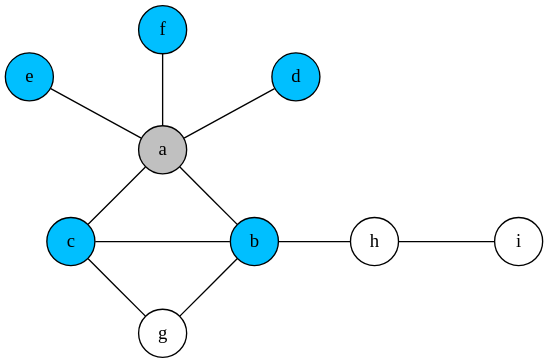
\includegraphics[width=0.5\textwidth]{MB_graph}
	\caption{The Markov Blanket of node 'a' consists of all blue nodes, as they are its direct neighbors.}
	
	\label{fig:MB_GGM}
\end{figure}

\citet{kaufmann_bayesian_2015} present an efficient Gibbs sampler for inferring the Markov Blanket for a small number of variables.
While following an approach similar to \citet{wang_bayesian_2012}, 
a conditional independence property in the likelihood is used for separating the inference of the Markov Blanket from the rest of the network.
Due to the reliance on computationally expensive \gls{MCMC} methods for the estimation, this is a highly useful property and makes the Bayesian approach to Covariance Selection feasible for bigger problem sizes (in terms of total network size).


In this Chapter we will provide an overview of \citet{kaufmann_bayesian_2015} and its most important properties.
The full model and its derivation are omitted for the sake of brevity and can be found in \autoref{A:model}.
Furthermore, we extend the sampler with Simulated Annealing for estimating the MAP instead of the whole posterior marginals.


\section{Bayesian Markov Blanket}
We stay in the setting of Gaussian Graphical Models.
Let $\W \in \mathbb{R}^{(p+q)}$ be a symmetric positive definite matrix.
Data $\matr{X}$ is assumed to be normally distributed with
$$
\matr{X} \sim \mathcal{N}_{(p+q)}(0,\W^{-1})
$$ 
Additionally, the observed data $X=(\matr{x_1}, \dots, \matr{x_{(p+q)}})$ with $\matr{x}_i\in\mathbb{R}^{n}$ is ordered such that the first $p$ columns correspond to query variables we are interested in, with $q$ corresponding to the remaining variables.
It is assumed that $p\ll q$.
Furthermore, $\matr{S}$ and $\matr{W}$ are partitioned into block matrices according to $p$ and $q$:
\begin{equation*}
\matr{W}=
\raisebox{0.3\baselineskip}{$
	\begin{blockarray}{ccc}
	p & q& \\
	\begin{block}{(cc)l}
	\matr{W}_{11} & \matr{W}_{12}&p \\
	\matr{W}_{12}^T & \matr{W}_{22}&q \\
	\end{block}
	\end{blockarray}
	$}
\quad \quad \quad \quad 
\matr{S}=
\raisebox{0.3\baselineskip}{$
	\begin{blockarray}{ccc}
	p & q& \\
	\begin{block}{(cc)l}
	\matr{S}_{11} & \matr{S}_{12}&p \\
	\matr{S}_{12}^T & \matr{S}_{22}&q \\
	\end{block}
	\end{blockarray}
	$}
\end{equation*}

The Markov Blanket of the query variables $p$ is now given by the block $\Wxy$.
As such, the aim is to estimate the precision matrix block $\Wxy$.
It is important to note that $\Sxx$ and $\Wxx$ are much smaller than $\Syy$ and $\Wyy$ respectively (given $p\ll q$).

The main motivation of the \gls{BMB} sampler is a block-wise factorization of the likelihood that effectively allows decoupling the inference of $\Wxy$ from the large matrix $\Wyy$.
By then constructing a prior admitting a similar factorization, the factorization can be propagated to the posterior which then reveals a block-wise conditional independence structure.

\subsection{Likelihood}
Let the sample Covariance be $\matr{S} = \matr{X}^T\matr{X}$.
As shown in \autoref{GRAPH_SELECTION}, the likelihood is of form
\begin{equation}
\label{eq:BMB_likelihood}
p(\matr{S}|\W) \propto \det(\matr{W}^{n/2}) \exp\tr\Big(-\frac{1}{2} \matr{WS}\Big)
\end{equation}
 which corresponds to a Wishart distribution:
$$
p(\matr{S}|\W) \propto \mathcal{W}_{p+q}(n,\matr{W})
$$
\citet{kaufmann_bayesian_2015} then show that the likelihood factorizes as shown in Lemma \autoref{lemma:ll}.

\begin{tcolorbox}[colback=yellow!5!white,colframe=yellow!75!black]
	\begin{customlemma}{1}[\cite{kaufmann_bayesian_2015}]
		\label{lemma:ll}
		Let $\Wyys = \Wyy - \Wyx\Wxx^{-1}\Wxy$ be the Schur complement of block $\Wxx$ in $\W$.
		Then the likelihood of the covariance matrix factorizes in terms of $\W$ as follows:
		$$
		\mathcal{L}_S(\matr{W}) \propto \mathcal{L}_1(\Wxx, \Wxy)\mathcal{L}_2(\Wyys)
		$$
	\end{customlemma}
\end{tcolorbox}
It should be noted that when seen as a function of $\W$, the likelihood is no proper \gls{pdf} 
\footnote{The integral of the likelihood over $\W$ is not equal to one: $\int \mathcal{L}_S(\matr{W}) \dif\W \neq 1$} 
and the factorization is as such only a functional statement.

We will not prove this factorization here but rather assume it, for constructing a prior. 
Subsequently the factorization can be shown in the full posterior.
This results in an arguably less convoluted derivation.

\subsection{Prior}
The prior for $\W$ has to ensure symmetry and positive-definiteness.
Consequently, a Wishart prior is chosen.
It is the natural conjugate prior to $p(\matr{S}|\matr{W})$ with its support being symmetric positive definite matrices.
But the Wishart alone is insufficient, as sparsity is to be enforced. 
For this, a \gls{DE} prior for the non-diagonal entries of $\matr{W}$ can be used.
To admit a block-wise factorization similar to the likelihood, the \gls{DE} prior is only placed on the non-diagonal entries of the $\Wxy$ block.
Analogous to \citet{wang_bayesian_2012}, the \gls{DE} prior is represented as a scale mixture of Gaussians (see \autoref{BGLASSO}) with inverse-Gaussian distributed scale parameters $\matr{T}=\{t_{ij}\}$.
\begin{align}
\label{eq:BMB_prior}
P(\matr{W}|\matr{T}) &=
\mathcal{W}_{p+q} \big(p + q + 1, \matr{I}\big) p(\matr{W}_{12} | \matr{T} )
\\
&\propto \exp\tr \Big(-\frac{1}{2} \matr{W}\Big)
\prod_{{\substack{i=1,\dots,p\\j=1,\dots,q}} }   \frac{1}{\sqrt{2\pi \matr{T}_{ij}}} \exp 
\Big( - \frac{(\matr{W}_{12})_{ij}^2}{2\matr{T}_{ij}} \Big) 
\nonumber\\ \nonumber\\
P(\matr{T}| \lambda) &\propto
\prod_{{\substack{i=1,\dots,p\\j=1,\dots,q}} }   \frac{\lambda^2}{2} \exp \Big( - \frac{\lambda^2}{2} \matr{T}_{ij} \Big)
\nonumber
\end{align}

\subsection{Factorization of the Posterior}
The joint distribution of the model arises from combining the compound prior in \autoref{eq:BMB_prior} with the likelihood given in \autoref{eq:BMB_likelihood}.

\begin{align*}
p(\matr{W}, \matr{S}, \matr{T} | \lambda) =& p(\matr{W}_{11}, \matr{W}_{12}, \matr{W}_{22}, \matr{S}, \matr{T} | \lambda) \\
\propto &\det(\matr{W})^{\frac{n}{2}}  \det(\matr{S})^{\frac{n-(p+q)-1}{2}} 
\\
&\exp\Bigg(-\frac{1}{2} \tr [\matr{WS}+\matr{W}] - \frac{1}{2} \sum_{{\substack{i=1,\dots,p\\j=1,\dots,q}} } \frac{(\matr{W}_{12})_{ij}^2}{\matr{T}_{ij}}  \Bigg) 
\\
&\times \Big[\prod_{{\substack{i=1,\dots,p\\j=1,\dots,q}} }  \frac{1}{\sqrt{2\pi \matr{T}_{ij}}}\Big]
p(\matr{T}|\lambda)
\end{align*}

Let the Schur complement of $\matr{W}_{11}$ in $\W$ be:
$$\matr{W}_{22.1} = \matr{W}_{22} - \matr{W}_{12}^T \matr{W}_{11}^{-1} \matr{W}_{12}$$

We can reparameterize the joint distribution by $(\matr{W}_{11}, \matr{W}_{12}, \matr{W}_{22.1})$, with the change of variable admitting a constant Jacobian:
$$ J\big((\matr{W}_{11}, \matr{W}_{12}, \matr{W}_{22}) \rightarrow (\matr{W}_{11}, \matr{W}_{12}, \matr{W}_{22.1})\big) = \matr{1} $$

With the new parameterization, the determinants and traces can be written as:
\begin{align*}
\det(\matr{W}) &= \det(\matr{W}_{11}) \det(\matr{W}_{22} - \matr{W}_{12}^T \matr{W}_{11}^{-1}\matr{W}_{12})
\\
&= \det(\matr{W}_{11}) \det(\matr{W}_{22.1})
\\
\\
\tr(\matr{WS}) &= \tr\big[\matr{W}_{11}\matr{S}_{11} + \matr{W}_{12}\matr{S}_{21} + \matr{W}_{21}\matr{S}_{12} + \matr{W}_{22}\matr{S}_{22}   \big]
\\
&= \tr\big[\matr{W}_{11}\matr{S}_{11} + \matr{W}_{12}\matr{S}_{12}^T + \matr{W}_{12}^T\matr{S}_{12} + (\matr{W}_{22.1} + \matr{W}_{12}^T\matr{W}_{11}^{-1}\matr{W}_{12}) \matr{S}_{22}   \big]
\\
&= \tr\big[
\Cline[blue]{\matr{W}_{11}\matr{S}_{11}} + 
\Cline[yellow]{\matr{W}_{12}\matr{S}_{12}^T + 
	\matr{W}_{12}^T\matr{S}_{12}} + 
\Cline[red]{\matr{W}_{22.1}\matr{S}_{22}} + 
\Cline[green]{\matr{W}_{12}^T\matr{W}_{11}^{-1}\matr{W}_{12}\matr{S}_{22}}   
\big]
\\
\\
\tr(\matr{W}) &= \tr(\matr{W}_{11}) + \tr(\matr{W}_{22})
\\
&= \tr(\Cline[blue]{\matr{W}_{11}}) + 
\tr(\Cline[red]{\matr{W}_{22.1}}) +
\tr(\Cline[green]{\matr{W}_{12}^T\matr{W}_{11}^{-1}\matr{W}_{12}})
\end{align*}
When plugged into the joint distribution, this results in:
\begin{align*}
p(\matr{W}_{11}, \matr{W}_{12}, &\matr{W}_{22.1}, \matr{S}, \matr{T} | \lambda) \propto
\\
&\det(\matr{W}_{11})^{n/2} \det(\matr{W}_{22.1})^{n/2} \det(\matr{\matr{S}})^{\frac{n-(p+q)-1}{2}}
\\
\times& \exp \Big(
-\frac{1}{2}
\tr\big[
\Cline[blue]{\matr{W}_{11} (\matr{S}_{11} + \matr{I}) }+ 
\Cline[red]{\matr{W}_{22.1}  (\matr{S}_{22} + \matr{I})} + 
\\
&\quad \quad \quad \quad \quad \quad
\Cline[yellow]{2 (\matr{W}_{12}^T\matr{S}_{12})} +
\Cline[green]{
	\matr{W}_{12}^T \matr{W}_{11}^{-1}\matr{W}_{12} 
	(\matr{S}_{22} + \matr{I})}
\big]
\Big)
\\
\times& \exp\Big(- \frac{1}{2} \sum_{{\substack{i=1,\dots,p\\j=1,\dots,q}} } \frac{(\matr{W}_{12})_{ij}^2}{\matr{T}_{ij}} \Big) \quad \Big[\prod_{{\substack{i=1,\dots,p\\j=1,\dots,q}} }  \frac{1}{\sqrt{2\pi \matr{T}_{ij}}}\Big]
\quad
p(\matr{T}|\lambda)
\\\\
%%%%%%%%%%%%%%%%%%%%%%%%%%%%%%%%%%%%%%%%%%%%%%%%%%%%%%%%%%%%%%%%%%%%%%%%%%%
=&\det(\matr{W}_{11})^{n/2} \det(\matr{\matr{S}})^{\frac{n-(p+q)-1}{2}} 
\\
\times& \exp \Big(
-\frac{1}{2}
\tr\big[
\Cline[blue]{\matr{W}_{11} (\matr{S}_{11} + \matr{I}) } +  
\Cline[yellow]{2 (\matr{W}_{12}^T\matr{S}_{12})} +
\Cline[green]{
	\matr{W}_{12}^T \matr{W}_{11}^{-1}\matr{W}_{12} 
	(\matr{S}_{22} + \matr{I})}
\big]
\Big)
\\
\times& \exp\Big(- \frac{1}{2} \sum_{{\substack{i=1,\dots,p\\j=1,\dots,q}} } \frac{(\matr{W}_{12})_{ij}^2}{\matr{T}_{ij}} \Big) \quad \Big[\prod_{{\substack{i=1,\dots,p\\j=1,\dots,q}} }  \frac{1}{\sqrt{2\pi \matr{T}_{ij}}}\Big]
\quad
p(\matr{T}|\lambda)
\\
\times& 
	\det(\matr{W}_{22.1})^{n/2} 
	\exp
	\Bigg(
		-\frac{1}{2}
		\tr
		\Big[
			\Cline[red]{\matr{W}_{22.1}  (\matr{S}_{22} + \matr{I})}
		\Big]
	\Bigg)
\end{align*}
In this formulation it's clear to see that by conditioning on $\Syy$, $\Wyys$ is (conditionally) independent of $\Wxx$ and $\Wxy$.
\begin{tcolorbox}[colback=red!5!white,colframe=red!60!black, title=Conditional Independence Property]
	The posterior distribution of $\W$ factorizes as follows:
	\begin{equation}
	p(\matr{W}_{11}, \matr{W}_{12}, \matr{W}_{22.1}, \matr{T} | \matr{S}, \lambda)
	= p(\matr{W}_{11}, \matr{W}_{12}, \matr{T} | \matr{S}, \lambda) p(\matr{W}_{22.1} | \matr{S}, \lambda) 
	\end{equation}
	This implies that the posterior of $(\Wxx, \Wxy)$ is conditionally independent of $\Wyys$, given $\matr{S}$:
	\begin{equation}
	\label{eq:W22}
	(\Wxx \text{,} \Wxy)\bigCI \Wyys | \matr{S}
	\end{equation}
\end{tcolorbox}
As a consequence, the Markov Blanket can be inferred independently of the prohibitively large $\Wyy$, using only the  joint posterior over $\Wxx$, $\Wxy$ and $\matr{T}$.

%The joint posterior over $\Wxx$, $\Wxy$ and $\matr{T}$ is then:
\begin{tcolorbox}[colback=red!5!white,colframe=red!60!black, title=Joint Posterior Distribution]
	\begin{align}
	\label{eq:jointpost}
		p(\matr{W}_{11}, \matr{W}_{12}, \matr{T} | \matr{S}, \lambda)
		\propto& \quad
		\det(\matr{W}_{11})^{n/2} \exp \Big( - \frac{1}{2} \tr\big[ \matr{W}_{11} (\matr{S}_{11} + \matr{I}) \big]\Big)
		\\
		&\times \exp\Bigg(
		-\frac{1}{2}\text{vec}(\matr{W}_{12})^T \Big[
		(\matr{S}_{22} + \matr{I}) \otimes \matr{W}_{11}^{-1} +\matr{D}\Big]\text{vec}(\matr{W}_{12})
		\nonumber\\&\quad \quad  \quad \quad \quad \quad 
		- \text{vec}(\matr{W}_{12})^T \text{vec}(\matr{S}_{12})
		\Bigg)
		\nonumber \\
		&\times \Big[\prod_{{\substack{i=1,\dots,p\\j=1,\dots,q}} }  \frac{1}{\sqrt{2\pi \matr{T}_{ij}}}\Big]
		p(\matr{T}|\lambda)
		\nonumber
	\end{align}
	Where $\matr{D} = \text{diag}(\text{vec}(\matr{T}))^{-1}$,
	i.e. $\matr{D}$ is a diagonal matrix with entries $(\matr{T}_{ij})^{-1}$.
\end{tcolorbox}

\subsection{Posterior Conditionals}

It can now be shown that each of the posterior conditionals of $\Wxx$, $\Wxy$, $\matr{T}$ and $\Wyys$ follows a known closed-form distribution.
While we may not be interested in $\Wyys$ (or $\Wyy$) directly,
it is required for embedding the \gls{BMB} in the copula sampler.

The resulting distributions are shown in the following overview, while the full derivation can be found in \autoref{A:post_cond}.
They are omitted at this point of the thesis for the sake of compactness.

\begin{tcolorbox}[colback=red!5!white,colframe=red!60!black, title= Posterior Conditional of $\Wxy$]
	\begin{enumerate}
		\item $\Wxy$ follows a multivariate Normal distribution:
		\begin{align}
		\text{vec}(\matr{W}_{12}) | \matr{W}_{11}, \matr{T}, \matr{S}, \lambda &\sim \mathcal{N}(-\matr{C}^{-1} \text{vec}(\matr{S}_{12}), \matr{C}^{-1})
		\\
		\matr{C} = \Big[
		(\matr{S}_{22} + \matr{I}) &\otimes \matr{W}_{11}^{-1} +\matr{D}\Big]
		\nonumber
		\end{align}
		With $\matr{D} = \text{diag}(\text{vec}(\matr{T}))^{-1}$\\
		It should be noted, that as a special case for $\matr{T}_{ij} \rightarrow \infty$, i.e.
		$\matr{D}\rightarrow \matr{0}$ the posterior simplifies to:
		$$
		\mathcal{N}\Big(-\text{vec}(\Wxx \Sxy (\Syy+\matr{I}) ^{-1}), 
		(\Syy + \matr{I})^{-1} \otimes \Wxx
		\Big)
		$$
		\item $\Wxx$ follows a \gls{MGIG} distribution:
		\begin{align}
		\Wxx | \Wxy, \matr{T}, \matr{S}, \lambda \sim 
		\mathcal{MGIG}_B
		\Big(
		\frac{n+p+1}{2}, \ 
		\Sxx+\matr{I},\  
		\Wxy(\Syy+I)\Wxy^T
		\Big)
		\end{align}
		(Using the parametrization of the \gls{MGIG} as presented by \citet{butler_generalized_1998})
		\item $\Wyys$ follows a Wishart distribution:
		\begin{align}
		\Wyys | \matr{S}, \lambda \sim \mathcal{W}\Big(
		n-\frac{p-1}{3}, \Syy
		\Big)
		\end{align}
		\item $(\matr{T}_{ij})^{-1}$ follow an inverse Gaussian distribution:
		\begin{align}
		(\matr{T}_{ij})^{-1} \sim \mathcal{IG}
		\Big(
		\mu' = \sqrt{
			\frac{\lambda^2}{(\matr{W}_{12})_{ij}^2}
		},
		\lambda' = \lambda^2
		\Big)
		\end{align}
	\end{enumerate}		
\end{tcolorbox}

While $\Wxy$, $\Wyys$ and $\matr{T}$ follow distributions that can be easily sampled, the \gls{MGIG} is more difficult.
\citet{bernadac_random_1995} shows that the \gls{MGIG} can be represented and sampled as a continued fraction of Wishart distributed Matrices.
But by its very nature, continued fractions of matrices are numerically unstable.
Consequently, finding an alternative representation of the posterior that does not rely on the \gls{MGIG} is favored.


\subsubsection{Posterior Marginal of $\Wxx$}
\label{ss:postmarginal}
The joint posterior of $\Wxx$ and $\Wxy$ can be split up using the chain rule:
$$ p(\Wxx, \Wxy | \matr{T}, \matr{S}, \lambda) = 
p(\Wxy | \Wxx, \matr{T}, \matr{S}, \lambda) p(\Wxx | \matr{T}, \matr{S}, \lambda)
$$
From the previous section, it is known that the posterior conditional of $\Wxy | \Wxx, \matr{T}, \matr{S}, \lambda$
is proportional to the exponential part of a normal distribution (for details see \autoref{A:post_cond}).
The marginal $p(\matr{W}_{11} |  \matr{T}, \matr{S}, \lambda)$ can then be computed by integrating out $\Wxy$.

For this step we utilize the fact that integrating over the unnormalized part of a Gaussian distribution results in its normalization constant. This is given by construction, since a \gls{pdf} has to integrate to one.
\begin{align*}
\int \mathcal{N}(x;\mu, \matr{\Sigma})\dif x=
&\int \frac{1}{\sqrt{(2\pi)^n\det(\boldsymbol\Sigma)}}
\exp\left(
-\frac{1}{2}({x}-{\mu})^T{\boldsymbol\Sigma}^{-1}({x}-{\mu})
\right)
\dif x
= 1
\\
\Rightarrow
&\int
\exp\left(
-\frac{1}{2}({x}-{\mu})^T{\matr{\Sigma}}^{-1}({x}-{\mu})
\right)
\dif x
= \sqrt{(2\pi)^n\det(\matr{\Sigma})}
\\
&\qquad\qquad\qquad\qquad\qquad\qquad\qquad\quad\quad\ 
\propto \sqrt{\det(\matr{\Sigma})}
\end{align*}

Now plugging the joint posterior \autoref{eq:jointpost} into the marginalization results in:
\begin{align*}
	 p(&\matr{W}_{11} |  \matr{T}, \matr{S}, \lambda)=\int p(\matr{W}_{11}, \matr{W}_{12} |  \matr{T}, \matr{S}, \lambda)\dif\Wxy
	\\
	&\propto 
	\int
	\det(\matr{W}_{11})^{n/2} \exp \Big( - \frac{1}{2} \tr\big[ \matr{W}_{11} (\matr{S}_{11} + \matr{I}) \big]\Big)
	\\
	&\times \exp\Bigg(
	-\frac{1}{2}\text{vec}(\matr{W}_{12})^T \Big[
	(\matr{S}_{22} + \matr{I}) \otimes \matr{W}_{11}^{-1} +\matr{D}\Big]\text{vec}(\matr{W}_{12})
	- \text{vec}(\matr{W}_{12})^T \text{vec}(\matr{S}_{12})
	\Bigg)
	\dif\Wxy
	\\\\
	&= 
	\det(\matr{W}_{11})^{n/2} \exp \Big( - \frac{1}{2} \tr\big[ \matr{W}_{11} (\matr{S}_{11} + \matr{I}) \big]\Big)
	\\
	&\times 
	\int
	\underbrace{
		\exp\Bigg(
		-\frac{1}{2}\text{vec}(\matr{W}_{12})^T \Big[
		(\matr{S}_{22} + \matr{I}) \otimes \matr{W}_{11}^{-1} +\matr{D}\Big]\text{vec}(\matr{W}_{12})
		- \text{vec}(\matr{W}_{12})^T \text{vec}(\matr{S}_{12})
		\Bigg)
	}_{\propto\mathcal{N}\big(-\matr{C}^{-1}\text{vec}(\Wxy), \matr{C}^{-1}\big)}
	\dif\Wxy		
	\\\\
	&\propto 
	\det(\matr{W}_{11})^{n/2} \exp \Big( - \frac{1}{2} \tr\big[ \matr{W}_{11} (\matr{S}_{11} + \matr{I}) \big]\Big)
	{\det(\matr{C})^{\frac{1}{2}}}
\end{align*}
\begin{tcolorbox}[colback=red!5!white,colframe=red!60!black, title=
	Posterior Marginal $\Wxx|\matr{T}\text{,}\matr{S}\text{,}\lambda$]
	\begin{equation*}
	p(\matr{W}_{11} |  \matr{T}, \matr{S}, \lambda)= 
	\det(\matr{W}_{11})^{n/2} \exp \Big( - \frac{1}{2} \tr\big[ \matr{W}_{11} (\matr{S}_{11} + \matr{I}) \big]\Big)
	\det
	\Big(
	(\matr{S}_{22} + \matr{I}) \otimes \matr{W}_{11}^{-1} +\matr{D}
	\Big)^{\frac{1}{2}}
	\end{equation*}
\end{tcolorbox}

To our knowledge, this offers no possibility of reformulation into some known closed-form distribution,
as the determinant arising from the normalization of $p(\Wxy | \Wxx, \matr{T}, \matr{S}, \lambda)$ cannot be split up.

For the special case $\matr{T}_{ij}\rightarrow0$, i.e. $\matr{D}\rightarrow\matr{0}$:
$$
\matr{C}\overset{D\rightarrow\matr{0}}{\rightarrow}
\big(
	(\Syy+I) \otimes \Wxx^{-1}
\big)
$$
\begin{align*}
\det
\Big(
	(\matr{S}_{22} + \matr{I}) \otimes \matr{W}_{11}^{-1}
\Big)^{\frac{1}{2}}
&\overset{\text{\tiny{(516 Matr. Cookbook)}}}{=}
\Big(
	\det(\Syy + \matr{I})^{\text{rank}(\Wxx^{-1})} 
	\det(\matr{W}_{11}^{-1})^{\text{rank}(\Syy+\matr{I})}
\Big)^{\frac{1}{2}}
\\
&=
\Big(
\det(\Syy + \matr{I})^{p} 
\det(\matr{W}_{11}^{-1})^{q}
\Big)^{\frac{1}{2}}
\\
&= 
\det(\Syy + \matr{I})^{\frac{p}{2}} 
\det(\matr{W}_{11})^{-\frac{q}{2}}
\end{align*}
As $\Wxx$  and $\Syy$ are symmetric positive definite matrices, they have full rank $p$ and $q$ respectively. 
It then also follows that $\text{rank}(\Syy + \matr{I})= \text{rank}(\Syy)$.

Then
\begin{align*}
 p(\matr{W}_{11} |  \matr{T}, \matr{S}, \lambda)
 &\overset{\matr{D}\rightarrow\matr{0}}{\propto}
\det(\matr{W}_{11})^{n/2} \exp \Big( - \frac{1}{2} \tr\big[ \matr{W}_{11} (\matr{S}_{11} + \matr{I}) \big]\Big)
\det(\matr{W}_{11})^{-{q}/{2}}
\\
&\ \  =
\det(\matr{W}_{11})^{(n-q)/2} \exp \Big( - \frac{1}{2} \tr\big[ \matr{W}_{11} (\matr{S}_{11} + \matr{I}) \big]\Big)
\end{align*}

Comparing the determinants to the Wishart Distribution($\Wxx$ is known to be of size $p$):
\begin{align*}
&\frac{1}{2}(df-p-1) = \frac{1}{2}(n-q)
\\
\Rightarrow &df = n-q+p-1
\end{align*}
$$\Downarrow$$
\begin{tcolorbox}[colback=red!5!white,colframe=red!60!black, title= $\Wxx|\matr{T}\text{,}\matr{S}\text{,}\lambda$ for special case $T_{ij}\rightarrow\infty$]
	\begin{equation}
	p(\matr{W}_{11} |  \matr{T}, \matr{S}, \lambda)
	\overset{\matr{D}\rightarrow\matr{0}}{\propto}
	\mathcal{W}(n-q+p-1, \matr{\Sxxs})
	\end{equation}
\end{tcolorbox}

\subsection{Gibbs Sampler}
With the posterior conditionals available, constructing a Gibbs sampler is straightforward.
Furthermore, the sampler can be expanded by the semi-parametric Gaussian copula for relaxing the assumption of Gaussian marginals.
For the extension, the Wishart draw of the precision matrix in the copula sampler 
(see Algorithm \autoref{alg:copula}) is to be replaced by a draw of $\W$ from the \gls{BMB}.
At this step, the whole precision matrix and thus the $\Wyy$ block is needed.
Due to the factorization, $\Wyys$ can be sampled from a Wishart (See \autoref{eq:W22}) and subsequently be used to calculate $\Wyy$.

After obtaining the empirical posterior distribution with the Gibbs sampler, the zero-edges in the precision matrix are estimated by thresholding.
As sparse networks are wanted, we estimate entries of $\matr{W}$ as zero if they are deemed insignificant according to the Credible Interval (i.e. if the \gls{CI} of a certain level includes 0).
Significant entries of the precision matrix are then estimated by the median.

The full Gibbs sampler (including thresholding and the copula) is shown in Algorithm \autoref{alg:Gibbs_sampler}.

\begin{algorithm}[H]
	\caption{Gibbs Sampler using Semi-Parametric Gaussian Copula}\label{alg:Gibbs_sampler}
	
	{\fontsize{9}{12}\selectfont\begin{algorithmic}
				\Function{draw\_MB}{$\W, \matr{S}, \matr{T}, \lambda$}
				\State
				\textbf{Sample}		
				\Comment{\gls{BMB} Gibbs sweep}
				\State {}$\qquad\quad$
				$ 				(\matr{T}_{ij})^{-1} \sim \mathcal{IG}
				\Big(
				\mu' = \sqrt{
					\frac{\lambda^2}{(\matr{W}_{12})_{ij}^2}
				},
				\lambda' = \lambda^2
				\Big) $
				
				\State $\qquad\quad$
				$				\matr{W}_{11} | \matr{W}_{12}, \matr{T}, \matr{S}, \lambda \sim 
				\mathcal{MGIG}_B
				\Big(
				\frac{n+p+1}{2}, \ 
				\matr{S}_{11}+\matr{I},\  
				\matr{W}_{12}(\matr{S}_{22}+\matr{I})\matr{W}_{12}^T
				\Big)$
				\State $\qquad\quad$
				$ \text{vec}(\matr{W}_{12}) | \matr{W}_{11}, \matr{T}, \matr{S}, \lambda \sim \mathcal{N}(-\matr{C}^{-1} \text{vec}(\matr{S}_{12}), \matr{C}^{-1}) $
				\State $\qquad\quad$
				$
				\Wyys | \matr{S}, \lambda \sim \mathcal{W}\big(n-\frac{(p-1)}{3}, \Syy\big)
				$

				\State
				$
				\Wyy \gets \Wyys + \Wxy^T \Wxx^{-1} \Wxy
				$
				
				\State
				\Return($\W, \matr{T}$)
				\EndFunction
				\\
				
				\Function{draw\_latent\_scores}{$\matr{X}, \matr{W}, \matr{Z}, \matr{S}$}\Comment{{Draw random scores}}
				\For{$j = 1,\dots,(p+q)$}
				\State $\sigma^2_j \gets 1/\matr{W}_{j,j}$
				\For{$x \in unique\{x_{1,j}, \dots, x_{n,j}\}$}
				\State Find lower bound $a \gets \sup(z_{i,j} : x_{i,j} < x)$
				\State Find upper bound $b \gets \inf(z_{i,j} : x<x_{i,j})$
				\For{each $i$ such that $x_{i,j}=x$}
				\State $\mu_{i,j} \gets -\sigma_j^2 \matr{z}_{i,-j}\matr{S}_{-j,j}$
				\State Sample $z_{i,j} \sim \mathcal{TN}(\mu_{i,j}, \sigma_j^2, a, b)$
				\EndFor
				\EndFor
				\EndFor
				
				\State
				\Return{$(\matr{Z})$}
				\EndFunction
				\\
				\hrulefill
		\State {\textbf{BMB Gibbs Sampler}}
		\\
		\State \textbf{Input}: \\
		\quad\quad\quad\quad\quad
		$\matr{X}$ \qquad \quad\quad \ \ \  $n \times (p+q)$ data matrix containing observations from $(p+q)$ rvs
		\\
		\quad\quad\quad\quad\quad
		$\lambda>0$ \qquad \quad \ sparsity inducing hyper parameter
		\\
		\quad\quad\quad\quad\quad
		$thresh\_low$ \quad defines $[thresh\_low, 1-thresh\_low]$ Credible Interval
		\\
		\quad\quad\quad\quad\quad
		\textit{NSCAN} \qquad total number of Gibbs sweeps
		\\
		\quad\quad\quad\quad\quad
		\textit{BURNIN} \quad \ \ number of samples discarded for final estimation
		\\
		\State \textbf{Initialize}:\\
		\quad\quad\quad\quad\quad
		$\matr{W}^{(0)} \gets \lambda \matr{I}_{p+q}$
		\\
		\quad\quad\quad\quad\quad
		$\matr{Z}^{(0)} \gets 
		\Big\{
		{z}_{i,j} \gets \Phi^{-1}
		\Big(\frac{\text{rank}_i(x_{i,j})}{n_i+1} \Big)$ for $j\in \{1,\dots,(p+q)\}, i \in \{1,\dots,n\}
		\Big\}$
		\\
		\quad\quad\quad\quad\quad
		$\matr{S}^{(0)} \gets (\matr{Z}^{(0)})^T \matr{Z}^{(0)} $
		\\
		\quad\quad\quad\quad\quad
		Sample $\matr{W} \sim \mathcal{W}_{p+q}\Big(n, (S+W_0)^{-1}\Big) $
		%\For{$k = 1,\dots,N_{GibbsSamples}$}
		\\
		\For{$k=1,\dots,$\textit{NSCAN}}
		\State
		$\matr{Z}^{(k)} \gets$ \Call{draw\_latent\_scores}{$\matr{X}, \matr{W}^{(k-1)}, \matr{Z}^{(k-1)}, \matr{S}^{(k-1)}$}\Comment{Draw random scores}
		\State
		$ \matr{S}^{(k)} \gets (\matr{Z}^{(k)})^T\matr{Z}^{(k)} $
		\Comment{Update S}
		\State $(\W^{(k)}, \matr{T}^{(k)}) \gets \Call{draw\_MB}{\W^{(k-1)}, \matr{S}^{(k)}, \matr{T}^{(k-1)}, \lambda}$
		\Comment{Draw BMB Posterior Conditional}
		\EndFor
		\State
		\For{i,j=1,\dots,(p+q)}
		\Comment{Threshold and estimate}
			\State
			CI $\gets$ \Call{CredibleInterval}{$\W_{i,j}^{(burnin:NSCAN)},thresh\_low$}
				\If{$0 \in $ CI}
				\State
				$\hat{\W}_{i,j} \gets 0$
				\Else
				\State
				$\hat{\W}_{i,j} \gets \Call{median}{\W_{i,j}^{(burnin:NSCAN)}}$
				\EndIf
		\EndFor
		\\
		\State
		\textbf{Output:}
		\State $\qquad\qquad $ Estimated Precision Matrix $\hat{\W}$
	\end{algorithmic}}
\end{algorithm}

\section{Simulated Annealing}
The Gibbs sampler of \cite{kaufmann_bayesian_2015} allows us to investigate the whole posterior distribution of the \gls{BMB} model, making it possible to compute \gls{CI}s and other statistics of interest.
But ultimately, the \gls{MAP} estimate of the network is wanted, which corresponds to the point in the posterior having highest probability.
Even though MCMC provides the full posterior probability, it is still an empirical one, which leads to the need of multivariate density estimation for finding the mode.
However, it has been shown that multivariate density estimation is not feasible for high dimensional distributions due to the 'curse of dimensionality' \citep{scott1991feasibility}.
In addition, most of the samples drawn will not explore the region of the mode unless it is closely surrounded by the majority of probability mass.
Simulated Annealing solves this by allowing to approximately sample from the set of global maxima.
Thus, it can be used for estimating the \gls{MAP}.

It should be noted here, that the \gls{MAP} is not guaranteed to lead to the 'best' estimate for any problem but actually depends on the posterior distribution at hand.
If the posterior distribution is multi-modal or the majority of probability mass is far away from the mode, one might argue that the \gls{MAP} is not representative for the distribution. 
On the other hand, if the posterior distribution is unimodal with a lot of mass surrounding it, the \gls{MAP} might be preferable.
While we cannot claim this to be true in general,
experiments on artificial data indicate that the $\Wxy$ block of interest is unimodal for sufficiently high lambda.
We will expand on this in \autoref{ss:modality}.

\subsection{The Joint MAP}
\label{ss:joint_map}
First of all, it is important to distinguish which MAP we are actually estimating with the Simulated Annealing.
The posterior distribution that is sampled from in the original \gls{BMB} 
is
$
p(\W, \matr{T}| \matr{S}, \lambda)
$,
where $\lambda$ denotes the sparsity inducing hyperparameter.
Extending it with the semi-parametric Gaussian copula (\autoref{s:semi_copula}) leads to:
\begin{equation}
p(\W, \matr{T}, \matr{S} |\matr{Z}\in D, \lambda)
\end{equation}

As \gls{MCMC} sampling provides the full posterior distribution,
inference on $\W$ and more specifically $\Wxy$ is made on the marginals:
$$
p((\W)_{i,j}|\matr{Z}\in D, \lambda)
$$

On the other hand, with Simulated Annealing the auxiliary variables $\matr{T}$ and $\matr{Z}$ influence the MAP problem and the following joint \gls{MAP} is estimated:
$$
\arg\max_{\W, \matr{T}, \matr{S}} p(\W, \matr{T}, \matr{S} | \matr{Z}\in D, \lambda)
$$
It should be noted that the $\W$ resulting from this joint \gls{MAP} estimate is different from the \gls{MAP} of the marginal:
$$
\arg\max_{\W} p(\W|\matr{Z}\in D, \lambda)
$$

In our approach for the Annealing, the latent scores $\matr{Z}$ are first estimated by posterior mean with the Gibbs sampler:
$$
\hat{Z} = E[\matr{Z}|\matr{Z}\in D, \lambda] 
$$
Subsequently, $\matr{S}$ is fixed to
$$
\hat{S} = \hat{Z}^T\hat{Z}
$$
As $\Wyy$ was only necessary for the copula, the joint MAP we get when fixing the latent variables is:
$$
(\hat W_{11}, \hat W_{12}, \hat{T}) = \argmax_{(\Wxx, \Wxy, \matr{T})} p(\Wxx, \Wxy, \matr{T} | \hat{S}, \lambda)
$$
Aside from the unimodality mentioned before, it is now also not guaranteed that this joint \gls{MAP} estimate leads to a sparse estimate of $\Wxy$.
A similar problem in context of SA for generalized linear regression has been addressed by \citet{raman2012sparse}.
Through a variational formulation the joint MAP was shown to be identical to the marginal posterior for certain choices of a sparsity parameter (note, that this parameter has a different effect than the $\lambda$).
While we can offer no such proof, our experimental results suggest that the inferred networks are indeed sparse
for sufficiently high $\lambda$.

\subsection{Model}
For implementing the \gls{SA}, we make use of the method for extending a Gibbs sampler shown in \autoref{ss:SA}. 
As such, a cooling parameter $T_i$ is introduced to the posterior conditionals:
$$p(x_i|x_{-i})^{1/T_i}$$ 

With distributions that are part of the exponential family, the cooling only results in a shift of the parameters while retaining the general form. 
This is given for all posterior conditionals of the \gls{BMB}.
The following subsections show the derivation of the respective cooled down distributions.
To avoid confusion between the variables, the temperature parameter is from now on referred to as $\Tc$.
\subsubsection{Cooling of the Posterior Conditional $\Wxx$}
Let the Matrix Variate $\matr{X}$ be distributed according to the \gls{MGIG} (using the parameterization of \citet{butler_generalized_1998})
\begin{align*}
\bm{X} &\sim \mathcal{MGIG}_B(\lambda, A, B) \\
p({X}) &\propto \det({X})^{\lambda - \frac{1}{2}(p+1)}
\exp \tr
\Big(
-\frac{1}{2} (\matr{A}{X} + \matr{B} {X}^{-1} )
\Big)
\end{align*}

Then $p(X)^{1/T}$ can be written as
\begin{align*}
\Tc &\in \mathbb{R}_{>0}
\\
p(X)^{\frac{1}{\Tc}}
&\propto det(X)^{\frac{{\lambda - \frac{1}{2}(p+1)}}{\Tc}} exp \lbrack tr(-\frac{1}{2}(AX + BX^{-1} ))\rbrack^{\frac{1}{T}}
\\
&\propto det(X)^{\frac{\lambda}{\Tc} - \frac{1}{2\Tc}(p+1)} exp \lbrack tr(-\frac{1}{2\Tc}(AX + BX^{-1} ))\rbrack
\\
&\propto det(X)^{\frac{\lambda}{\Tc} - \frac{1}{2\Tc}(p+1)} exp \lbrack tr(-\frac{1}{2}(\frac{A}{\Tc}X + \frac{B}{\Tc}X^{-1} ))\rbrack
\\
&\propto det(X)^{\big({\frac{\lambda}{\Tc} - \frac{1}{2\Tc}(p+1)} + \frac{1}{2}(p+1)\big) - \frac{1}{2}(p+1)} exp \lbrack tr(-\frac{1}{2}(\frac{A}{\Tc}X + \frac{B}{\Tc}X^{-1} ))\rbrack
\\
&\propto det(X)^{\big(\frac{\lambda}{\Tc} + \frac{p+1}{2}(1-\frac{1}{\Tc})\big) - \frac{1}{2}(p+1)} exp \lbrack tr(-\frac{1}{2}(\frac{A}{\Tc}X + \frac{B}{\Tc}X^{-1} ))\rbrack
\\
&\propto p(Y) 
\\
\bm{Y} &\sim \mathcal{MGIG}_B\Bigg(\Big(\frac{\lambda}{\Tc} + \frac{p+1}{2}\big(1-\frac{1}{\Tc}\big)\Big), \ \frac{A}{\Tc},\ \frac{B}{\Tc}\Bigg)
\end{align*}

Now we can express the posterior conditional of $\Wxx$ as follows.

\begin{tcolorbox}[colback=red!5!white,colframe=red!60!black, title=Cooled Posterior Conditional of $\Wxx$]
	\begin{align}
		p\big(\Wxx | \Wxy, \matr{T}, \matr{S}, \lambda\big)^{1/\Tc} \propto 
		\mathcal{MGIG}_B
		\Big(
		\frac{\frac{n}{\Tc}+p+1}{2}, \ 
		\frac{\Sxx+\matr{I}}{\Tc},\  
		\frac{\Wxy(\Syy+I)\Wxy^T}{\Tc}
		\Big)
	\end{align}
\end{tcolorbox}

\subsubsection{Cooling of the Posterior Conditional $\Wxy$}
Let $\matr{X}$ be a normally distributed (vector) random variable:
\begin{align*}
\boldsymbol{X} &\sim N(\boldsymbol{\mu}, \matr{\Sigma})
\\
p(\boldsymbol{x}) &= \big( (2\pi)^k \det{(\matr{\Sigma})}\big)^{-\frac{1}{2}} exp \lbrack - \frac{1}{2} (\boldsymbol{x}-\boldsymbol{\mu})^t \matr{\Sigma}^{-1} (\boldsymbol{x}-\boldsymbol{\mu}) \rbrack
\end{align*}
Then introducing the cooling temperature $\Tc$ leads to:
\begin{align*}
\Tc &\in \mathbb{R}_{>0} 
\\
p(x)^{\frac{1}{\Tc}}&= \big( (2\pi)^k \det{(\Sigma)}\big)^{-\frac{1}{2\Tc}} 
exp \lbrack - \frac{1}{2} (\boldsymbol{x}-\boldsymbol{\mu})^T \matr{\Sigma}^{-1} (\boldsymbol{x}-\boldsymbol{\mu}) \rbrack^{\frac{1}{\Tc}}
\\
&\propto exp \lbrack - \frac{1}{2} (\boldsymbol{x}-\boldsymbol{\mu})^T \matr{\Sigma}^{-1} (\boldsymbol{x}-\boldsymbol{\mu}) \rbrack^{\frac{1}{\Tc}}
\\
&\propto exp \lbrack - \frac{1}{2\Tc} (\boldsymbol{x}-\boldsymbol{\mu})^T \matr{\Sigma}^{-1} (\boldsymbol{x}-\boldsymbol{\mu}) \rbrack
\\
&\propto exp \lbrack - \frac{1}{2} (\boldsymbol{x}-\boldsymbol{\mu})^T \frac{\matr{\Sigma}^{-1}}{\Tc} (\boldsymbol{x}-\boldsymbol{\mu}) \rbrack
\\
&\propto exp \lbrack - \frac{1}{2} (\boldsymbol{x}-\boldsymbol{\mu})^T (\Tc \matr{\Sigma})^{-1} (\boldsymbol{x}-\boldsymbol{\mu}) \rbrack
\\
&\propto p(y) 
\\
Y &\sim \mathcal{N}(\boldsymbol{\mu}, \Tc \matr{\Sigma})
\end{align*}
\begin{tcolorbox}[colback=red!5!white,colframe=red!60!black, title=Cooled Posterior Conditional of $\Wxy$]
\begin{align}
p\big(\text{vec}(\matr{W}_{12}) | \matr{W}_{11}, \matr{T}, \matr{S}, \lambda\big)^{1/\Tc} &\propto \mathcal{N}(-\matr{C}^{-1} \text{vec}(\matr{S}_{12}), \Tc\matr{C}^{-1})
\\
\matr{C} = \Big[
(\matr{S}_{22} + \matr{I}) &\otimes \matr{W}_{11}^{-1} +\matr{D}\Big]
\nonumber
\end{align}
\end{tcolorbox}

\subsubsection{Cooling of the Posterior Conditional $\matr{T}$}
Let the \gls{IG} distribution be denoted by
$$
{X} \sim \mathcal{IG}(\mu, \rho)
$$
$$
p(x) = \Big(\frac{\rho}{2\pi x^3}\Big)^{1/2}\exp \Big[ \frac{-\rho(x-\mu)^2}{2\mu^2 x} \Big]
$$
and the \gls{GIG} distribution by
$$
{Y} \sim \mathcal{GIG}(a, b, p)
$$
$$
p(y) = \frac{(a/b)^{p/2}}{2K_p(\sqrt{ab})} y^{(p-1)} \exp\Big[-\frac{1}{2}\big(ay + \frac{b}{y}\big)\Big]
$$

The \gls{IG} distribution can be written as a special case of the \gls{GIG}:
\\
With  
\begin{equation}
{Y} \sim \mathcal{GIG}(a=\frac{\rho}{\mu^2}, b=\rho, p=-\frac{1}{2})
\label{IG_as_GIG_t}
\end{equation}
we get
$$p(x\geq\bm{X}) = p(x\geq\bm{Y})$$

As a consequence, the cooled $\mathcal{IG}$ can be written in terms of the $\mathcal{GIG}$:
\begin{align*}
p(y) &\propto
y^{(p-1)} \exp\Big[-\frac{1}{2}\big(ay + \frac{b}{y}\big)\Big]
\\
\\
\Tc &\in \mathbb{R}_{>0}
\\
p(y)^\frac{1}{\Tc} &\propto
y^{\frac{(p-1)}{\Tc}} \exp\Big[-\frac{1}{2\Tc}\big(ay + \frac{b}{y}\big)\Big]
\\
&\propto 
y^{(\frac{p-1}{\Tc}+1)-1} \exp\Big[-\frac{1}{2}\Big(\frac{a}{\Tc}y + \frac{b/\Tc}{y}\Big)\Big]
\\
&\propto p(z)
\end{align*}
$$
{Z} \sim \mathcal{GIG}\bigg(a'=\frac{a}{\Tc}, b'=\frac{b}{\Tc}, p'=\Big(\frac{p-1}{\Tc}+1\Big)\bigg)
$$
Plugging in the parameters of the \gls{IG} (\autoref{IG_as_GIG_t}) then leads to:
\begin{equation}
{Z} \sim \mathcal{GIG}\bigg(a'=\frac{\lambda/\mu^2}{\Tc}, b'=\frac{\lambda}{\Tc}, p'=\Big(-\frac{1.5}{\Tc}+1\Big)\bigg)
\end{equation}

Finally, the cooled down \gls{IG} posterior can be expressed as a \gls{GIG} distribution. 
\begin{tcolorbox}[colback=red!5!white,colframe=red!60!black, title=Cooled Posterior Conditional of $\matr{T}$]
	
		\begin{align}
 				p\big((\matr{T}_{ij})^{-1}\big)^{1/\Tc} \propto \mathcal{GIG}
\Big(
a = \frac{(\matr{W}_{12})_{ij}^2}{\Tc} ,
%\frac{\lambda^2}{\sqrt{
%		\frac{\lambda^2}{(\matr{W}_{12})_{ij}^2}
%	}^2},
b = \frac{\lambda^2}{\Tc},
p = \big(-\frac{1.5}{\Tc}+1\big)
\Big) 
		\end{align}
\end{tcolorbox}

\subsection{Cooling Schedule}
For the sake of simplicity, a geometric cooling schedule was chosen.
While different (non-adaptive) schedules were examined at first, we could not observe any significant differences.
The cooling schedule used corresponds to the one presented in \autoref{ss:SA}:

\begin{tcolorbox}[title=Geometric Cooling Schedule (2)]
	\begin{equation}
	f_T(i) = T_0  \Big(\frac{T_n}{T_0}\Big)^{i/n} \quad \quad i = 0,1,\dots,n
	\end{equation}
\end{tcolorbox}

\subsection{Sampler}
With the cooled down posterior conditionals and a cooling schedule available, the sampler can be constructed.

The sampler consists of three phases:

\begin{enumerate}
	\item 
	Running the Gibbs sampler for the \gls{BMB} with the copula.
	
	This part serves both as burn-in and for the estimation of the latent scores.
	The sample covariance $\matr{S}$ is estimated from the mean of the copula draws.
	\item 
	The Annealing itself.
	
	Starting at temperature $T_0=1$, the system is slowly cooled down to the target temperature $T_n$ according to the cooling function $f_T$.
	\item
	Sampling from the cooled down system.
	
	At the final temperature $T_n$ the sampling is continued for a small number of iterations, to sample from an area closely surrounding the mode. The \gls{CI}s of these samples are then finally used for estimating $\matr{W}$.
\end{enumerate}
The complete Simulated Annealing process for the \gls{BMB} is given in Algorithm \autoref{alg:SA_sampler}.


\FloatBarrier
\pagebreak
\begin{algorithm}[H]
	\caption{Simulated Annealing of the Bayesian Markov Blanket}\label{alg:SA_sampler}
	
	{\fontsize{9}{12}\selectfont\begin{algorithmic}
			\Function{draw\_MB\_cooled}{$\Wxx, \Wxy, \matr{S}, \matr{T}, \lambda, \Tc$}
			\State
			\textbf{Sample}		
			\State {}$\qquad\quad$
			$ 				(\matr{T}_{ij})^{-1} \sim \mathcal{GIG}
			\Big(
			a = \frac{(\matr{W}_{12})_{ij}^2}{\Tc} ,
			%\frac{\lambda^2}{\sqrt{
			%		\frac{\lambda^2}{(\matr{W}_{12})_{ij}^2}
			%	}^2},
				b = \frac{\lambda^2}{\Tc},
				p = \big(-\frac{1.5}{\Tc}+1\big)
			\Big) $
			
			\State $\qquad\quad$
			$				\matr{W}_{11} | \matr{W}_{12}, \matr{T}, \matr{S}, \lambda \sim 
			\mathcal{MGIG}_B
			\Big(
			\frac{\frac{n}{\Tc}+p+1}{2}, \ 
			\frac{\Sxx+\matr{I}}{\Tc},\  
			\frac{\Wxy(\Syy+I)\Wxy^T}{\Tc}
			\Big)$
			\State $\qquad\quad$
			$ \text{vec}(\matr{W}_{12}) | \matr{W}_{11}, \matr{T}, \matr{S}, \lambda \sim \mathcal{N}(-\matr{C}^{-1} \text{vec}(\matr{S}_{12}), \matr{C}^{-1}) $
			\State
			\Return($\Wxx, \Wxy, \matr{T}$)
			\EndFunction
			\\
			\hrulefill
			\State {\textbf{BMB Simulated Annealing}}
			\\
			\State \textbf{Input}: \\
			\quad\quad\quad\quad\quad
			$\matr{X}$ \qquad \quad\quad \ \ \  $n \times (p+q)$ data matrix containing observations from $(p+q)$ rvs
			\\
			\quad\quad\quad\quad\quad
			$\lambda>0$ \qquad \quad \ sparsity inducing hyper parameter
			\\
			\quad\quad\quad\quad\quad
			$thresh\_low$ \quad defines $[thresh\_low, 1-thresh\_low]$ Credible Interval
			\\
			\quad\quad\quad\quad\quad
			$N_{BMB}, N_{SA}$ \  number of BMB and SA iterations
			\\
			\quad\quad\quad\quad\quad
			$N_{CD}$ \qquad \quad \ \ number of draws from cooled down posterior
			\\
			\quad\quad\quad\quad\quad
			\textit{BURNIN} \quad \ \ number of samples discarded for final estimation
			\\
			\quad\quad\quad\quad\quad
			$T_0, T_n$  \qquad \quad initial and final temperature
			\\
			\State \textbf{Initialize}:\\
			\quad\quad\quad\quad\quad
			$\matr{W}^{(0)} \gets \lambda \matr{I}_{p+q}$
			\\
			\quad\quad\quad\quad\quad
			$\matr{Z}^{(0)} \gets 
			\Big\{
			{z}_{i,j} \gets \Phi^{-1}
			\Big(\frac{\text{rank}_i(x_{i,j})}{n_i+1} \Big)$ for $j\in \{1,\dots,(p+q)\}, i \in \{1,\dots,n\}
			\Big\}$
			\\
			\quad\quad\quad\quad\quad
			$\matr{S}^{(0)} \gets (\matr{Z}^{(0)})^T \matr{Z}^{(0)} $
			\\
			\quad\quad\quad\quad\quad
			Sample $\matr{W} \sim \mathcal{W}_{p+q}\Big(n, (S+W_0)^{-1}\Big) $
			%\For{$k = 1,\dots,N_{GibbsSamples}$}
			\\
			\LeftComment{BMB Gibbs Sampler (See Algorithm \autoref{alg:Gibbs_sampler})}
			\For{$k=1,\dots,N_{BMB}$}
			\State
			$\matr{Z}^{(k)} \gets$ \Call{draw\_latent\_scores}{$\matr{X}, \matr{W}^{(k-1)}, \matr{Z}^{(k-1)}, \matr{S}^{(k-1)}$}
			\State
			$ \matr{S}^{(k)} \gets (\matr{Z}^{(k)})^T\matr{Z}^{(k)} $
			\State $(\W^{(k)}, \matr{T}^{(k)}) \gets \Call{draw\_MB}{\W^{(k-1)}, \matr{S}^{(k)}, \matr{T}^{(k-1)}, \lambda}$
			\EndFor
			\\
			\State $\hat{Z} \gets \Call{MEAN}{\matr{Z}^{(burnin:N)}}$
			\Comment{Estimate and fix $S$}
			\State $\hat{S} \gets \hat{Z}^T \hat{Z}$
			\\
			\LeftComment{Simulated Annealing}
			\For{$k=(N_{BMB}+1),\dots, (N_{BMB} + N_{SA} - N_{CD})$}
			\State $\Tc^{(k)} = f_T(k-N_{BMB}-1)$
			\State $(\Wxx^{(k)}, \Wxy^{(k)}, \matr{T}^{(k)}) \gets \Call{draw\_MB\_cooled}{\Wxx^{(k-1)}, \Wxy^{(k-1)}, \hat{S}, \matr{T}^{(k-1)}, \lambda, \Tc^{(k)}}$
			\EndFor
			\\
			\LeftComment{Draw from cooled distribution}
			\For{$i=(k+1),\dots, (N_{BMB} + N_{SA} + N_{CD})$}
			\State $(\Wxx^{(i)}, \Wxy^{(i)}, \matr{T}^{(i)}) \gets \Call{draw\_MB\_cooled}{\Wxx^{(i-1)}, \Wxy^{(i-1)}, \hat{S}, \matr{T}^{(i-1)}, \lambda, \Tc^{(k)}}$
			\EndFor
			\State
			\LeftComment{Threshold and estimate}
			\For{i,j=1,\dots,(p+q)}
			\State
			CI $\gets$ \Call{CredibleInterval}{$\W_{i,j}^{(k:END)},thresh\_low$}
			\If{$0 \in $ CI}
			\State
			$\hat{\W}_{i,j} \gets 0$
			\Else
			\State
			$\hat{\W}_{i,j} \gets \Call{median}{\W_{i,j}^{(k:END)}}$
			\EndIf
			\EndFor
			\\
			\State
			\textbf{Output:}
			\State $\qquad\qquad $ Estimated Precision Matrix $\hat{\W}$
		\end{algorithmic}}
	\end{algorithm}

\subsection{Relation between Sparsity Hyperparameters}
For relating the regularization parameter $\rho$ of the Graphical LASSO to the $\lambda$ of the \gls{BMB} we refer to the result of Chapter 4.5.3 in \citet{kaufmann2017semi}.
By comparing the posterior of the \gls{BMB} with the regularized likelihood of the GLASSO, it is concluded that:
$$\lambda = \frac{n}{2}\rho$$
where $n$ refers to the number of data samples.
Because of the same model underlying both the \gls{BMB} and the \gls{SA}, it is reasonable to assume that the respective $\lambda$ are similar.

\chapter{Implementation}
In this chapter, details regarding the implementation of the samplers and the general setup of the artifical data used for evaluating the models are presented.
The Bayesian Markov Blanket and its SA extension were both implemented in Python 3 with the SciPy stack \citep{scipy}.
The code is openly available at
\begin{center}
	\href{https://github.com/FabricioArendTorres/BayesianMarkovBlanket/}{https://github.com/FabricioArendTorres/BayesianMarkovBlanket/}
\end{center}

\section{Sampling}
While SciPys statistics library includes many distributions to sample from,
more uncommon ones such as the GIG and MGIG are not covered.
Furthermore, SciPy relies on inverse transform sampling as a default sampling procedure,
which might not be optimal in terms of speed or numerical precision.
For the truncated normal distribution new sampling approaches have emerged that improve those aspects. 
As such they are preferable for the implementation of an MCMC sampler.
Last but not least, even for simple distributions such as the Normal distribution it can be beneficial to exploit the structure of the parameters for more efficient sampling procedures.
In this section we will expand on the methods used for sampling from the respective distributions in the presented Gibbs sampler.

\subsection{Normal Distribution: $\Wxy$}
\label{W12_draw}
We want to draw samples from:
\begin{align*}
	\text{vec}(\matr{W}_{12}) | \matr{W}_{11}, \matr{T}, \matr{S}, \lambda & \sim \mathcal{N}(-\matr{C}^{-1} \text{vec}(\matr{S}_{12}), \matr{C}^{-1}) 
	\\
	\matr{C} = \Big[
	(\matr{S}_{22} + \matr{I})                                             & \otimes \matr{W}_{11}^{-1} +\matr{D}\Big]                                 
\end{align*}

A naive approach would require the inversion of $\matr{C}$, a $(pq)\times(pq)$ matrix, where $q$ is known to be rather large.
This should be avoided, as the inversion is computationally expensive.

Instead we can sample from the transpose using Theorem \autoref{th:231}.
\begin{tcolorbox}[colback=yellow!5!white,colframe=yellow!75!black]
	\begin{customthm}{2.3.1}[\cite{gupta2018matrix}, Chapter 2.3]
		\label{th:231}
		If $\matr{X} \sim \mathcal{N}_{p,n}(\matr{M}, \matr{\Sigma} \otimes \matr{\Psi})$ then $\matr{X}^T \sim \mathcal{N}_{n,p}(\matr{M}^T, \matr{\Psi} \otimes \matr{\Sigma})$
	\end{customthm}
\end{tcolorbox}

This leads to:
\begin{tcolorbox}[colback=red!5!white,colframe=red!60!black]
	\begin{align*}
		\text{vec}(\matr{W}_{12}^T) | \matr{W}_{11}, \matr{T}, \matr{S}, \lambda & \sim \mathcal{N}(-(\matr{C'})^{-1} \text{vec}(\matr{S}_{12}^T), (\matr{C'})^{-1}) 
		\\
		\matr{C'} = \Big[
		\matr{W}_{11}^{-1}                                                       & \otimes (\matr{S}_{22} + \matr{I})+\matr{D}\Big]                                  
	\end{align*}
\end{tcolorbox}
where $\matr{C}'$ now admits a block-wise structure that can be exploited for an efficient Cholesky decomposition (as shown by \citet{kaufmann_bayesian_2015}).

Let $\matr{Q}=\Wxx^{-1}$
and $\matr{D} = \text{diag}(\matr{D}_1,\dots,\matr{D}_p)$.
then:
\[
	\matr{C}'=
	\begin{bmatrix}
		Q_{11}(\Syy+\matr{I})+\matr{D}_1 & \dots & Q_{1j}(\Syy+\matr{I}) & \dots & Q_{1p}(\Syy+\matr{I})              \\
		\vdots                           &       &                       &       & \vdots                             \\
		Q_{i1}(\Syy+\matr{I})            &       & \ddots                &       & Q_{ip}(\Syy+\matr{I})              \\
		\vdots                           &       &                       &       & \vdots                             \\
		Q_{p1}(\Syy+\matr{I})            & \dots & Q_{pj}(\Syy+\matr{I}) & \dots & Q_{pp}(\Syy+\matr{I}) + \matr{D}_p 
	\end{bmatrix}
\]

A block-wise Cholesky decomposition of the form
$$
\matr{C}' = \matr{L} \matr{L}^T
$$
is then given by

\newcommand{\syyi}{(\Syy + \matr{I})}
\newcommand{\blockunw}[1]{\Big(Q_{#1#1}\syyi+\matr{D}_#1\Big)}
\[
	\matr{L}^T=
	\begin{bmatrix}
		\matr{K}_1^\frac{1}{2} & Q_{12} \matr{B}_1      & \cdots & Q_{1j} \matr{B}_1      & \cdots & Q_{1p} \matr{B}_1      \\
		\matr{0}               & \matr{K}_2^\frac{1}{2} & \cdots & Q_{2j} \matr{B}_2      & \cdots & Q_{2p} \matr{B}_2      \\
		\vdots                 & \vdots                 & \ddots & \vdots                 &        & \vdots                 \\
		\matr{0}               & \matr{0}               & \cdots & \matr{K}_j^\frac{1}{2} & \cdots & Q_{jp} \matr{B}_j      \\
		\vdots                 & \vdots                 &        & \vdots                 & \ddots & \vdots                 \\
		\matr{0}               & \matr{0}               & \cdots & \matr{0}               & \cdots & \matr{K}_p^\frac{1}{2} 
	\end{bmatrix}
\]
with
\begin{align*}
	\matr{K}_i & = \blockunw{i}                   
	\\
	\matr{B}_i & = \matr{K}_i^{-\frac{1}{2}}\syyi 
\end{align*}

Non-diagonal entries only differ by a (scalar) factor $Q_{ij}$, which allows for an efficient computation by reusing the $\matr{B}_i$.
The $\matr{K}_i^{\frac{1}{2}}$ can be calculated by a naive Cholesky decomposition as $\matr{K}_i$ are symmetric positive definite.

For drawing from the Normal distribution we can simply draw from a standard Normal Distribution and then transform it by multiplying with the standard deviation and adding the mean \cite[Chapter 7.4]{gentle2009computational}.
In our context this corresponds to Algorithm \autoref{alg:MN_sampler},
where the mean and standard deviation are calculated from the above mentioned block-wise Cholesky decomposition.



\begin{algorithm}[]
	\caption{Draw Sample from $\mathcal{N}\big(-(\matr{C'})^{-1} \text{vec}(\matr{S}_{12}^T), \matr{C'}^{-1}\big)$}\label{alg:MN_sampler}
	\begin{algorithmic}
		\Function{draw\_W12}{$\Wxx, \Syy, \matr{D}$}
		\\
		\State Compute $\matr{L} \gets BlockChol(\Wxx^{-1}, \Syy, \matr{D})$
		\\
		\State Solve for $y$: $\qquad \matr{L}y=-\text{vec}(\Sxy^T) $ 
		\Comment{using forward substitution}
		\State Solve for $\mu$: $\qquad \matr{L}^T\mu=y$
		\Comment{using backward substitution}
		\\
		\State Sample $\qquad\quad\ \  r \sim \mathcal{N}(0,\matr{I}_{pq})$
		\State Solve for $b$: $\qquad \matr{L}^T b=r$
		\Comment{using backward substitution}
		%		\\
		\State
		\Return $(b+\mu)$
		\Comment{$(b+\mu)\sim \mathcal{N}\big( -(\matr{C'})^{-1} \text{vec}(\matr{S}_{12}^T), \matr{C'}^{-1}\big)$}
		\EndFunction
	\end{algorithmic}
\end{algorithm}


\subsection{Matrix Generalized Inverse Gaussian: $\Wxx$}
\label{sample_MGIG}
For the $\Wxx$ block we have to sample from
$$
\matr{W}_{11} | \matr{W}_{12}, \matr{T}, \matr{S}, \lambda \sim 
\mathcal{MGIG}_B
\Big(
\lambda' = \frac{n+p+1}{2}, \ 
\matr{A} = \matr{S}_{11}+\matr{I},\  
\matr{B} = \matr{W}_{12}(\matr{S}_{22}+I)\matr{W}_{12}^T
\Big)
$$
\citet{bernadac_random_1995} has shown that the \gls{MGIG} can be represented as a continued fraction of Wishart random variables.  
Similar to \citet{kaufmann2017semi} we make use of this result for the sampling process.
\begin{tcolorbox}[colback=yellow!5!white,colframe=yellow!75!black]
	\begin{theorem_51but}
		Let $\matr{X}, \matr{Y}_1, \matr{Y}_2$ be independent random variables,
		\\
		such that
		$$
		\mathcal{L}(\matr{Y}_1) = \mathcal{W}_p(2k, \matr{B'}^{-1})
		\quad \quad
		\mathcal{L}(\matr{Y}_2) = \mathcal{W}_p(2k, \matr{A'}^{-1})
		\quad \quad
		k > \frac{p-1}{2}
		$$
		$$
		\mathcal{L}(\matr{X}) = \mathcal{MGIG}_B\big(-k, \matr{A'}, \matr{B'} \big)
		$$
		$$
		\text{iff} \quad \mathcal{L}(\matr{X}) = \mathcal{L}((\matr{Y}_1 + (\matr{Y}_2 + \matr{X})^{-1})^{-1})
		$$
	\end{theorem_51but}
\end{tcolorbox}
However, the condition for $\lambda'$ does not hold in our given MGIG distribution:
$$
k = -\frac{n+p+1}{2} < \frac{p-1}{2} \qquad \text{\Lightning}
$$

It is important to note at this point, that the relation between the degrees of freedom $-\lambda' = 2df$ arises from comparing the determinant of the Wishart to the determinant of the MGIG reparameterized by its inverse in \autoref{propos_34}.
\begin{tcolorbox}[colback=yellow!5!white,colframe=yellow!75!black]
	\begin{propos_34but}
		\begin{equation}
			\label{propos_34}
			\mathcal{L}(\matr{X}) = \mathcal{MGIG}_B(\lambda', \matr{A}', \matr{B}') 
			\Leftrightarrow 
			\mathcal{L}(\matr{X}^{-1}) = \mathcal{MGIG}_B(-\lambda', \matr{B}', \matr{A}')
		\end{equation}
	\end{propos_34but}
\end{tcolorbox}

For addressing the constraint issue, the MGIG is written in terms of the parameterization by Letac (similar to the \gls{GIG} formulation in \cite{letac1983characterization}):
\begin{equation*}
	\matr{X} \sim \mathcal{MGIG}_{L}(n', \matr{A}, \matr{B}) 
\end{equation*}
\begin{equation}
	\label{eq:MGIG_L}
	p(\matr{X}) \propto \det(\matr{X})^{-n' - 1}
	\exp \tr
	\Big(
	-\frac{1}{2} (\matr{A}\matr{X} + \matr{B} \matr{X}^{-1} )
	\Big)
\end{equation}
with the condition now being \cite[Appendix 4]{kaufmann2017semi}:
$$
n'>\frac{p-1}{2}
$$
A change of variable to its inverse with $\matr{W}=\matr{X}^{-1}$ with Jacobian $det(\matr{W})^{-(p+1)}$ 
leads to:
\begin{align}
	p(\matr{W}) & \propto \det(\matr{W}^{-1})^{-n' - 1} 
	\exp \tr
	\Big(
	-\frac{1}{2} (\matr{A}\matr{W}^{-1} + \matr{B} \matr{W} )
	\Big)
	\nonumber
	\\
	            & = \det(\matr{W})^{n'-p}               
	\exp \tr
	\Big(
	-\frac{1}{2} (\matr{A}\matr{W}^{-1} + \matr{B} \matr{W} )
	\Big)
	\label{eq:inverse_MGIG}
\end{align}
If the posterior conditional is now expressed in terms of \autoref{eq:inverse_MGIG},
the corresponding inverse formulated as in \autoref{eq:MGIG_L} fulfills the constraint
and we can sample from this inverse.

With the posterior conditional being (see \autoref{A:post_cond} for details)
\[
	p(\matr{W}_{11} | \matr{W}_{12}, \matr{T}, \matr{S}, \lambda)
	\propto
	\det(\matr{W}_{11})^{n/2}
	\exp \Big(
	-\frac{1}{2} \tr\big[
		(\matr{S}_{11}+ \matr{I})\matr{W}_{11} + \matr{W}_{12}(\matr{S}_{22}+\matr{I})\matr{W}_{12}^T \matr{W}_{11}^{-1}
	\big]
	\Big)
\]
a comparison with \autoref{eq:inverse_MGIG} gives
\begin{align*}
	A              & =  \matr{W}_{12}(\matr{S}_{22}+\matr{I})\matr{W}_{12}^T 
	\\
	B              & = \matr{S}_{11}+ \matr{I}                               
	\\
	\frac{n}{2}    & = n'-p                                                  \\
	\Rightarrow n' & = \frac{n}{2}+p                                         
\end{align*}
So the inverse of our posterior conditional is
$$
\matr{W}_{11}^{-1} | \matr{W}_{12}, \matr{T}, \matr{S}, \lambda \sim \mathcal{MGIG}_L\Big(n'=\frac{n}{2}+p, A=(\matr{W}_{12}(\matr{S}_{22}+\matr{I})\matr{W}_{12}^T), B=(\matr{S}_{11}+ \matr{I}) \Big)
$$
For this inverse, the required constraint is satisfied:
$$
n' = \frac{n}{2}+p > \frac{(p-1)}{2}
$$

For sampling from the inverse, the determinant of this \gls{MGIG} is compared to the determinant of the Wishart distribution.
\begin{align*}
	n'-1=\frac{n}{2}+p-1 & = \frac{df-p-1}{2} 
	\\
	\Rightarrow df       & = n+3p-1           
\end{align*}
Finally, a sample can be drawn by the following continued fraction
$$
X = \Big((Y_1)_1 + 
\Big((Y_2)_1 + 
\Big( (Y_1)_2 + 
\Big( (Y_2)_2 + \dots \Big)^{-1} 
\Big)^{-1} 
\Big)^{-1}
\Big)^{-1}
$$
$$
(\matr{Y}_1)_i 
\sim 
\mathcal{W}_p
\Big(
n+3p-1, 
(\Wxy(\matr{S}_{22}+\matr{I})\Wxy^T)^{-1}
\Big)
\quad \quad
(\matr{Y}_2)_i 
\sim 
\mathcal{W}_p 
\Big(
n+3p-1, 
(\matr{S}_{11}+\matr{I})^{-1}
\Big)
$$
and then inverting the result:
$$
\Wxx = {X}^{-1}
$$

As we are drawing the inverse of the r.v. we are interested in, simply omitting the last inversion in the continued fraction leads to the desired result.
\subsubsection*{Simulated Annealing}
In case of the Simulated Annealing, the cooled posterior conditional is 
\[
	p(\matr{W}_{11} | \matr{W}_{12}, \matr{T}, \matr{S}, \lambda)^{1/\Tc}
	\propto
	\det(\matr{W}_{11})^{n/(2\Tc)}
	\exp \Bigg(
	-\frac{1}{2} \tr\Big[
		\frac{(\matr{S}_{11}+ \matr{I})}{\Tc}\matr{W}_{11} + \frac{\matr{W}_{12}(\matr{S}_{22}+\matr{I})\matr{W}_{12}^T}{\Tc} \matr{W}_{11}^{-1}
	\Big]
	\Bigg)
\]
Consequently the comparison with the inverted MGIG in \autoref{eq:inverse_MGIG} is slightly different:
\begin{align*}
	A              & =  \frac{\matr{W}_{12}(\matr{S}_{22}+\matr{I})\matr{W}_{12}^T }{\Tc} 
	\\
	B              & = \frac{\matr{S}_{11}+ \matr{I}}{\Tc}                                
	\\
	\frac{n}{2\Tc} & = n'-p                                                               \\
	\Rightarrow n' & = \frac{n}{2\Tc}+p                                                   
\end{align*}
Note, that the constraint is still satisfied for any $\Tc>0$:
$$
n' = \frac{n}{2\Tc}+p > \frac{(p-1)}{2}
$$
Comparing the determinant with the Wishart:
\begin{align*}
	n'-1=\frac{n}{2\Tc}+p-1 & = \frac{df-p-1}{2}   
	\\
	\Rightarrow df          & = \frac{n}{\Tc}+3p-1 
\end{align*}
Finally, a sample can be drawn by the following continued fraction
$$
X = \Big((Y_1)_1 + 
\Big((Y_2)_1 + 
\Big( (Y_1)_2 + 
\Big( (Y_2)_2 + \dots \Big)^{-1} 
\Big)^{-1} 
\Big)^{-1}
\Big)^{-1}
$$
$$
(\matr{Y}_1)_i 
\sim 
\mathcal{W}_p
\Bigg(
\frac{n}{\Tc}+3p-1, 
\Big(
\frac{\matr{W}_{12}(\matr{S}_{22}+\matr{I})\matr{W}_{12}^T }{\Tc}
\Big)^{-1}
\Bigg)
\quad \quad
(\matr{Y}_2)_i 
\sim 
\mathcal{W}_p 
\Bigg(
\frac{n}{\Tc}+3p-1, 
\Big(
\frac{\Sxx+ \matr{I}}{\Tc}
\Big)^{-1}
\Bigg)
$$
and then inverting the result:
$$
\Wxx = {X}^{-1}
$$
\subsection{Truncated Normal Distribution}
The inverse transform sampling implemented in SciPy fails and returns infinity for bounds that are far away from the mean.
Dependent on the data, this can break the copula Gibbs sampler, so an alternative method is required.
In the original implementation of the BMB by \citet{kaufmann_bayesian_2015}, the rejection sampler by \citet{geweke1991efficient} was used.
We follow a more recent approach presented by \citet{chopin2011fast}.
Compared to the rejection sampler, it offers slightly higher precision and speed.
Furthermore it does not require a table setup for sampling values from a new set of parameters.
In context of the copula, this is obviously a useful property as the scores are sampled from a new set of parameters each iteration.

\subsection{Generalized Inverse Gaussian}
For the GIG we utilize the sampler of the R package \textit{GIGrvg}
\footnote{\href{https://cran.r-project.org/web/packages/GIGrvg/}{https://cran.r-project.org/web/packages/GIGrvg/}}.
It is based on three different algorithms, each of which has performance advantages for specific ranges of the parameter values. 
The algorithms have been introduced by \citet{hormann2014generating} and \citet{lehner1989erzeugung} (which is a version of \citet{dagpunar1989easily} with a faster setup).

Alternative approaches may be faster for sampling multiple values from fixed parameters, but require a much longer setup. 
As mentioned before, this is disadvantageous in our setting.

The code was included by wrapping a C++ implementation\footnote{\href{https://github.com/horta/gig}{https://github.com/horta/gig}} of the R code in Cython. It is openly available via
\begin{center}
	\href{https://github.com/FabricioArendTorres/gig}{https://github.com/FabricioArendTorres/gig}
\end{center}

\section{Artificial Data: Setup and Metrics}
For evaluating the performance of the different network reconstruction methods, a data set that reflect the properties of the networks encountered in real applications is required.

We base the creation of the artificial data on the setup of \citet{kaufmann_bayesian_2015},
which will be described in the subsequent section.
For measuring how well the networks are reconstructed, a simple approach based on counting correctly predicted edges is followed.

\subsection{Data Setup}
\label{subs:artdata}

Each artificial data set is created by drawing 1000 samples from a zero-mean normal distribution 
$
\mathcal{N}_{p+q}(\matr{0}, \W^{-1})
$
with $p=10$ and $q=90$.
The structure of $\W$ is created according to a beta-binomial model.
That is, we first draw from the beta distribution
$$
\matr{\pi}_i \sim Beta(\alpha=0.01, \beta=1) \qquad i=1,\dots,(p+q)
$$
and then use the $\pi$ for drawing from a binomial
$$
{n}_{ij} \sim Bin(n=1, p=\pi_i) \qquad j = 1, \dots,(p+q)
$$
where ${n}_{ij}=1$ indicates that $\W_{ij}$ is non-zero and vice-versa.
As $E[\pi] = \frac{\alpha }{(\alpha+\beta)} = \frac{1}{101}$, the resulting network will be mostly sparse (i.e. have few edges) with only few nodes having a high $\pi$.
The few that have a higher $\pi$ will then exhibit a lot of edges to other nodes, resulting in a small-world structure of the network.

This sampling process can be repeated until a neighborhood structure fulfilling specific requirements is created.
In our case, those requirements are limits for the number of neighbors in $\Wxy$ and $\Wyy$:
\begin{enumerate}
	\item $5p < \sum\limits_{i=1}^{p} \sum\limits_{j=p+1}^{p+q}{n}_{ij} < q$
	\item $q < \sum\limits_{i=p+1}^{p+q} \sum\limits_{j=p+1}^{p+q}{n}_{ij} < 2q$
\end{enumerate}
The first requirement implies, that the fraction of non-zero edges lies between $\frac{5p}{pq}$ and $\frac{1}{p}$.
For $p=10$ and $q=10$ this means that $90\%$ to $94.\overline{4}\%$ of the edges in $\Wxy$ are zero. 

Finally, the edge weights are calculated by drawing uniformly from $[0.3,1]$ and then randomly flipping the sign of the weight:
\begin{align*}
	        & w_{ij} \sim \mathcal{U}(0.3, 1) \\
	        & f_{ij} \sim \mathcal{U}(-1,1)   
	\\
	\W_{ij} & = {n}_{ij} * w_{ij}  * sgn(f)   
\end{align*}

The resulting networks exhibits many connections to a few selected nodes, similarly to the real-world problems we target.
An example network is shown in \autoref{fig:example_newtork}.

\begin{figure}[H]
	\centering
	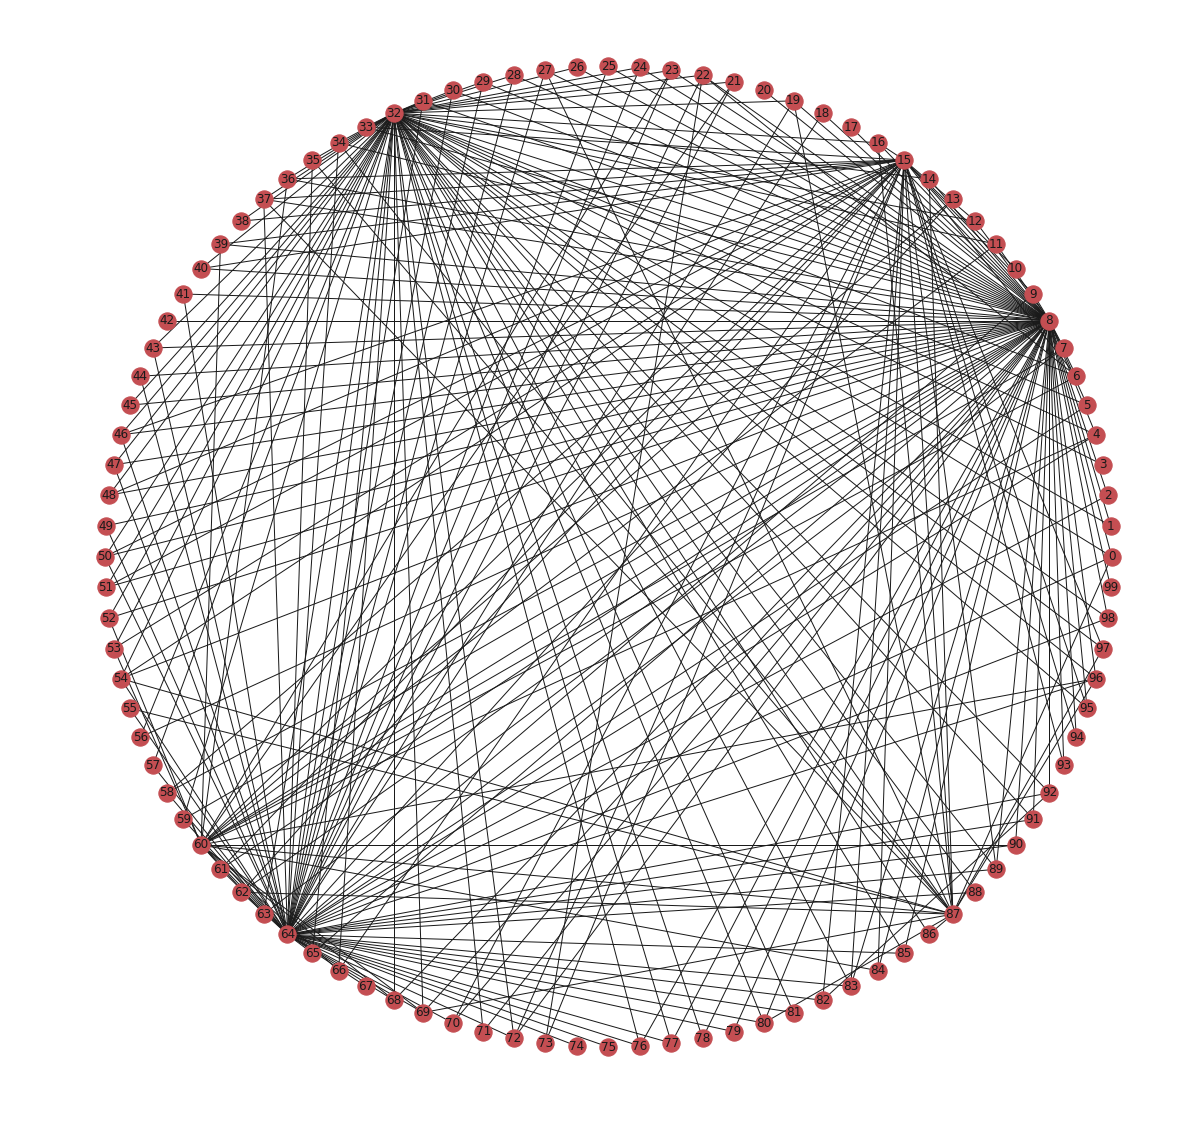
\includegraphics[width=0.48\textwidth]{data_fullgraph.png}
	\caption{Example network for $p=10$ and $q=90$, ordered such that the first $10$ nodes correspond to $p$. It can be seen that the network exhibits small-world properties in form of a few highly connected nodes, both in the $p$ as well as in the $q$ variables.}
		
	\label{fig:example_newtork}
\end{figure}

\subsection{Performance Metrics}
The metrics used for measuring the performance should be focused on how the structure of the predicted network graph compares to the ground truth.
But the problem of quantifying dissimilarities between graphs is in itself a difficult and computationally expensive one.
Instead we follow the simple approach of counting the prediction errors.
Similarly to \cite{kaufmann_bayesian_2015}, prediction of an (existing) edge with the wrong sign is counted as a false positive, as shown in the following confusion matrix.
\begin{table}[H]
	\centering
	\resizebox{0.8\textwidth}{!}{%
		\begin{tabular}{cccccc}
			&&&\multicolumn{3}{c}{\textbf{Actual}} 
			\\
			  &                  &   & $(\Wxy)_{i,j}<0$ & $(\Wxy)_{i,j}>0$ & $(\Wxy)_{i,j}=0$ 
			\\
			%\cmidrule{4-5}
			\multirow{3}{*}{\textbf{Predicted}}
			  & $(\Wxy)_{i,j}<0$ &   & TP               & FP               & FP               \\
			  & $(\Wxy)_{i,j}>0$ &   & FP               & TP               & FP               \\
			  & $(\Wxy)_{i,j}=0$ &   & FN               & FN               & TN               
		\end{tabular}}
\end{table}
On this basis, commonly known metrics such as the sensitivity (recall), specificity and precision can be calculated:

\begin{align*}
	sensitivity & = \frac{TP}{TP+FN} \\
	specificity & = \frac{TN}{TN+FP} \\
	precision   & = \frac{TP}{TP+FP} 
\end{align*}

As there is always a trade-off between these, we also look at the F-score and the Matthews correlation coefficient.
The F score is the harmonic mean between precision and recall, while the MCC is a measure of correlation between the predicted and the actual values \citep{baldi2000assessing}.

\[
	F = \frac{2TP}{2TP + FP + FN}
\]\\
\[
	MCC = \frac{TP \times TN - FP \times FN}{\sqrt{(TP + FP) (TP + FN) (TN+FP) (TN+FN)}}
\]


\chapter{Results}
With the models established, we focus on their application.
First, the performance and general behavior of the \gls{BMB}, the Simulated Annealing and the Graphical LASSO will be compared on artificial data. 
In the subsequent section we apply the BMB and SA in context of HIV-1.
The SystemsX.ch HIV-X cohort \citep{HIVX} provides data of long-term patients whose viral reservoir were successfully suppressed with antiretroviral therapy.
Our main goal is to find possible interactions between the resistance relevant mutations gathered from the viral genotype and multiple clinical factors that quantify the success of the treatment.


\section{Application on Artificial Data}
We compare the Graphical LASSO, the Bayesian Markov Blanket and its Simulated Annealing variant on multiple artificial data sets, created as described in \autoref{subs:artdata}. 
In addition, we look at the behavior of the posterior distribution of $\Wxy$ experimentally for different values of $\lambda$.

In \autoref{fig:toy_example}, a small example for two synthetic data sets with $p=5$ and $q=15$ is shown.
Both the SA and the BMB were used for reconstructing the Markov Blanket of the $p$ query variables, with $lambda=70$ and $\lambda=1400$ respectively.
\begin{figure}[H]
	\centering
	\subfloat{
		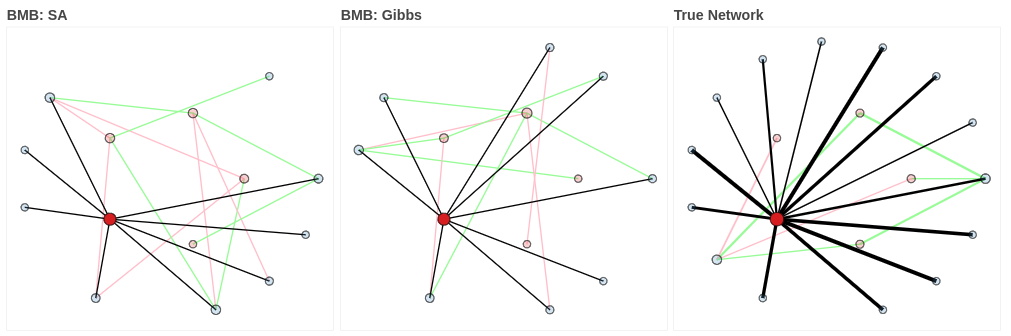
\includegraphics[width=1\linewidth]{network_ex_5_15}
	}
	\subfloat{
		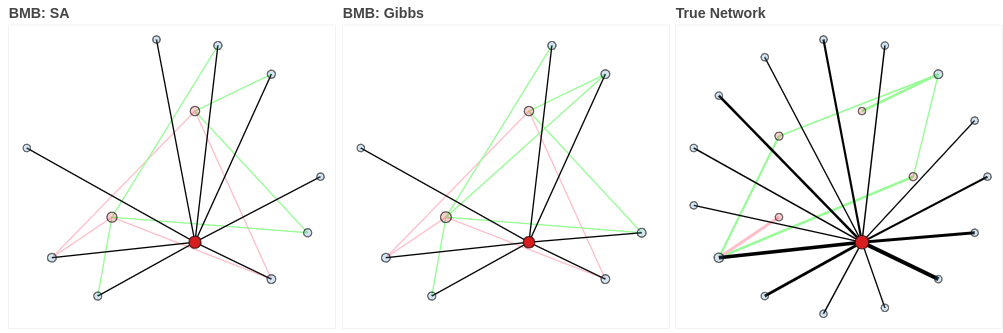
\includegraphics[width=1\linewidth]{network_ex_5_15_2}
	}
	\caption{Comparison of the true W12 subnetwork with the one resulting from the BMB ($lambda=70$) and SA ($\lambda=1400$) for two example networks with a threshold of $0.2$. The data was created similarly to the description in \autoref{subs:artdata}, but with $p=5$ and $q=15$.
		The red nodes correspond to the $p$ query variables.}
	
	\label{fig:toy_example}
\end{figure}
It can be seen that both networks are very similar, even though widely different $\lambda$ were used.
This is unexpected as the underlying model for both methods is the same.
In practice, finding an appropriate $\lambda$ is the most relevant part of the model selection,
as it is the only hyperparameter directly influencing the model.
Because of this, our focus in all three models will be the sparsity inducing hyperparameter and its effect on the quality of the reconstructed networks.

\subsection{Setup \& Model Hyperparameters}
Aim of the tests on the artificial data is a sound comparison between the original BMB and its Simulated Annealing variant.
As such, the methods should be set up in a similar way to avoid performance advantages simply due to parameter fine-tuning or the use of more computing resources (in our case iterations/sweeps) for either one.
The latter is especially important in the case of MCMC sampling and Simulated Annealing, where strong theoretical results for convergence exist.

We fix the number of total iterations in both samplers to 3000.
In the case of SA this refers to the summed amount of initial Gibbs sweeps, cooling steps and the draws from the cooled down system at temperature $T_n$.
As a consequence the computational effort is roughly equal between the two methods
\footnote{Only roughly, as the cooling part of the SA does not entail draws from the copula.}.
The detailed settings are shown in \autoref{table:settings_model}.
It should be noted that the burn-in is in both cases $0.3$ times the number of Gibbs Sweeps.

\begin{table}[H]
	\centering
	\caption{Model Parameters used for Testing\label{table:settings_model}}
	\begin{tabular}{l c c}
		& \textbf{BMB}   & \textbf{Simulated Annealing} \\
		\toprule
		Total Iterations  & $3000$         & $3000$                       \\\midrule
		Gibbs Sweeps      & $3000$         & $900$                        \\
		Burn-In           & $900$          & $270$                        \\
		Credible Interval & $[0.15, 0.85]$ & $[0.15, 0.85]$               \\
		Cooling Steps     & -              & $2100$                       \\
		Draws at $T_n$    & -              & $300$                        \\
		$T_0$             & -              & $1$                          \\
		$T_n$             & -              & $0.01$                       
	\end{tabular}
\end{table}

With these settings, the models were applied to 40 artificially created data sets with $p=10$ and $q=90$.

\subsection{Restrictions on Lambda}
\autoref{fig:sparsitybylambda} displays the average fraction of zero-edges (i.e. a measure of sparsity) of the reconstructed networks in relation to the chosen $\lambda$.
\begin{figure}
	\centering
	\subfloat{
		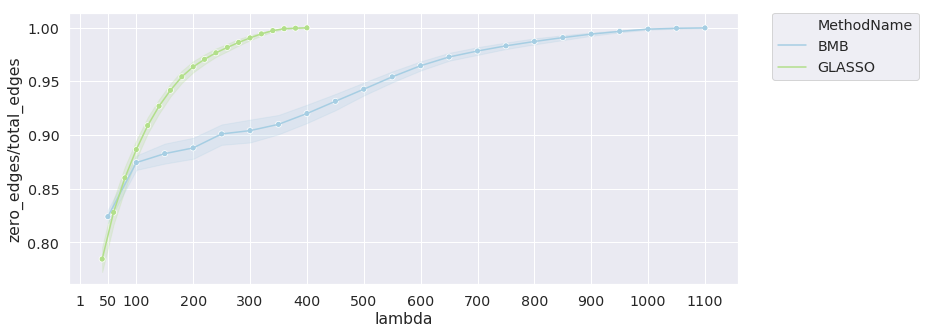
\includegraphics[width=0.9\linewidth]{sparsity_bylambda_GLBMB}
	}
	\subfloat{
		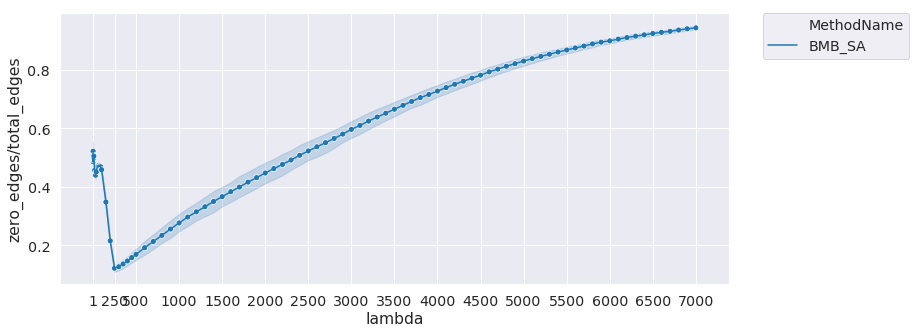
\includegraphics[width=0.9\textwidth]{sparsity_bylambda_SA}
	}
	
	\caption{Sparsity of Networks for different $\lambda$ over all 40 data sets.
		Plotted points correspond to the mean over all datasets and error bars to a $95\%$ bootstrapping confidence interval for the mean.}
	\label{fig:sparsitybylambda}
\end{figure}
The $\lambda$ were restricted to ranges that result in non-trivial (i.e. not empty) graphs. 
Furthermore, computational issues cause a lower bound for the GLASSO and an upper bound for the SA.
Lambdas below $100$ led to convergence problems for the Graphical LASSO, even in the case of a high number ($50000$) of iterations.
Conversely, SA has an upper bound due to numerical instability.
With increasingly high $\lambda$ the MGIG draws of the $\Wxx$ block (see \autoref{sample_MGIG}) and more specifically the inversion
$$
A=(\Wxy(\matr{S}_{22}+\matr{I})\Wxy^T)^{-1}
$$
fails as $A^{-1}$ becomes nearly singular.
We suspect the continued fraction of Wisharts to be a major cause of numerical instability in the sampler.
Decreasing the number of fractions used for sampling the MGIG increases the maximum possible $\lambda$ before failure, supporting this assumption.
While all three methods generally follow the trend of getting sparser for higher $\lambda$, the scale on which this happens is vastly different. 
Especially the Simulated Annealing requires a much higher $\lambda$ for the same level of sparsity as the BMB and GLASSO.
Aside from that, the BMB and SA behave differently than expected for very low $\lambda$.
Both recreate denser networks again, with the effect being more pronounced in the Annealing.
A problem possibly underlying this can be identified by comparing the MCMC diagnostic plots for the different $\lambda$.
\autoref{fig:diag_SA_l7000} shows the MCMC diagnostics for SA with a $\lambda$ of 7000.
\begin{figure}[H]
	\centering
	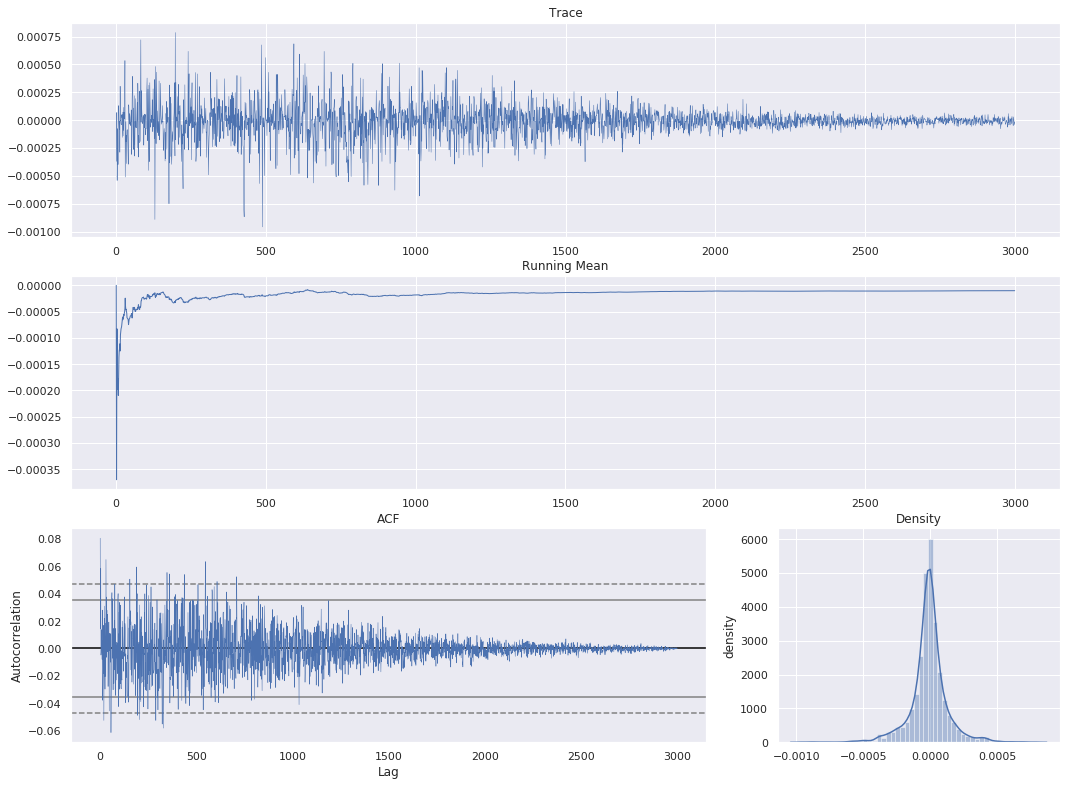
\includegraphics[width=0.7\textwidth]{diag_SA_l7000}
	\caption{MCMC Diagnostics: Simulated Annealing with a $\lambda$ of 7000}
	for the posterior marginal $(\Wxy)_{14}$.
	\label{fig:diag_SA_l7000}
\end{figure}
In the trace plot we can clearly see the effect of the Annealing.
Starting at iteration 1000, the system cools down and the samples slowly focus more on the region around the MAP.
Furthermore, the density plot indicates the marginal being unimodal%
\footnote{Note that the density plots of the Annealing includes \textit{all} drawn samples and only serves an diagnostic purpose.
	The actual estimation is only based on samples drawn at the target temperature.}.
When switching to a low $\lambda$ (see \autoref{fig:diag_SA_l20}), the cooled down chain starts fluctuating between two points,
which is also reflected in the very high autocorrelation switching signs for each lag.
As Simulated Annealing eventually samples from all global maxima, this behavior as well as the density plot indicates a multi-modality in the posterior marginals.
This effect gets more pronounced for smaller $\lambda$ as shown in \autoref{fig:diag_SA_l20},
where the distance between the modes also increases.
Since the modes seemingly diverge further from each other for lower $\lambda$, the Credible Interval also increases and is more likely to cover the origin, estimating an edge as 0.
This might explain the sparser networks for very small $\lambda$.

\begin{figure}
	\centering
	\subfloat{
		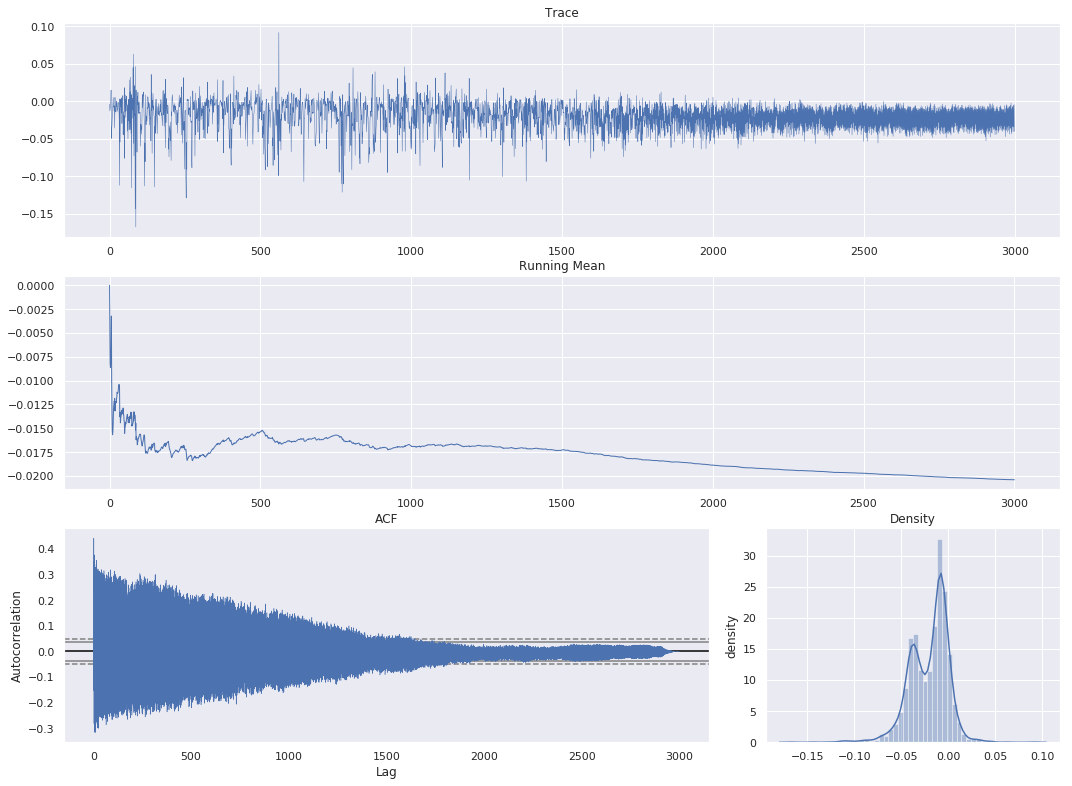
\includegraphics[width=0.8\linewidth]{diag_SA_l90}
	}
	\subfloat{
		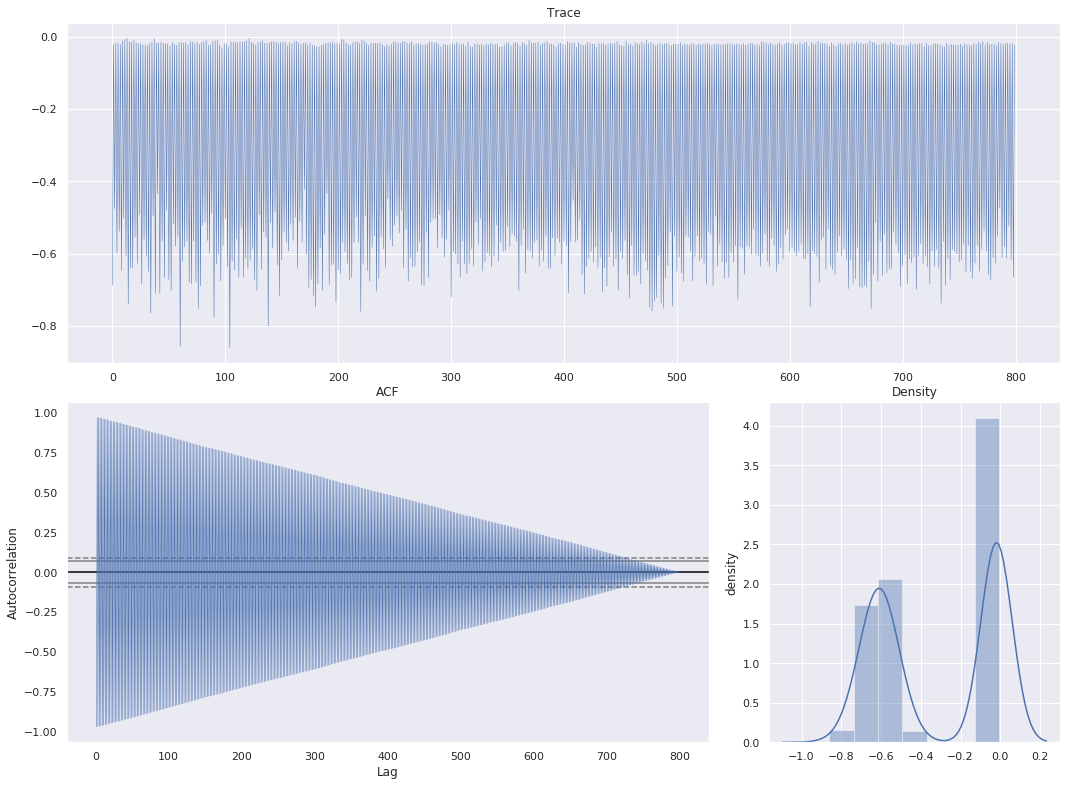
\includegraphics[width=0.8\textwidth]{diag_SA_l20}
	}
	\caption{MCMC Diagnostics: Simulated Annealing with a $\lambda$ of 90 (top) and 20 (bottom) }
	for the posterior marginal $(\Wxy)_{14}$.
	\label{fig:diag_SA_l20}
\end{figure}
In case of the standard BMB this behavior appears more subtle, but is still existent and can be observed for extremely small $\lambda$ (see \autoref{fig:diag_GIBBS_l1_400}).
But in this case, a high autocorrelation and jumping between values indicate mixture problems of the Markov chain. A possible cause might be numerical problems for low $\lambda$.
The hyperparameter $\lambda$ indirectly affects the diagonal of $\matr{C}$, which has to be inverted for draws of the $\Wxy$ block (see \autoref{W12_draw}).
However, the Markov chains corresponding to $\lambda$ in the range of $200$ to $300$ (where the bimodality in the SA marginals begins) did not exhibit similar problems, and neither could we observe any bimodal behavior in the non-cooled marginals.
%TODO

So the question arises whether multi-modality in the posterior actually exists for low $\lambda$ ($<300$) or just occurs as a side-effect of the Markov chains convergence problems.
In the next section we will expand on this by looking the empirical posteriors of $\Wxy$ for relatively small $\lambda$ that do not exhibit unusual behavior of the Markov chain.

Regardless of the outcome, it can already be seen that the $\lambda$s below $300$ do not lead to reasonable estimates 
for SA with the current thresholding method based on Credible Intervals.
Because of this, they will be disregarded for the performance evaluation in \autoref{ss:quality}.
Furthermore, $\lambda$ below $50$ will be ignored for the Gibbs BMB due to convergence problems.

\begin{figure}
	\centering
	\subfloat{
		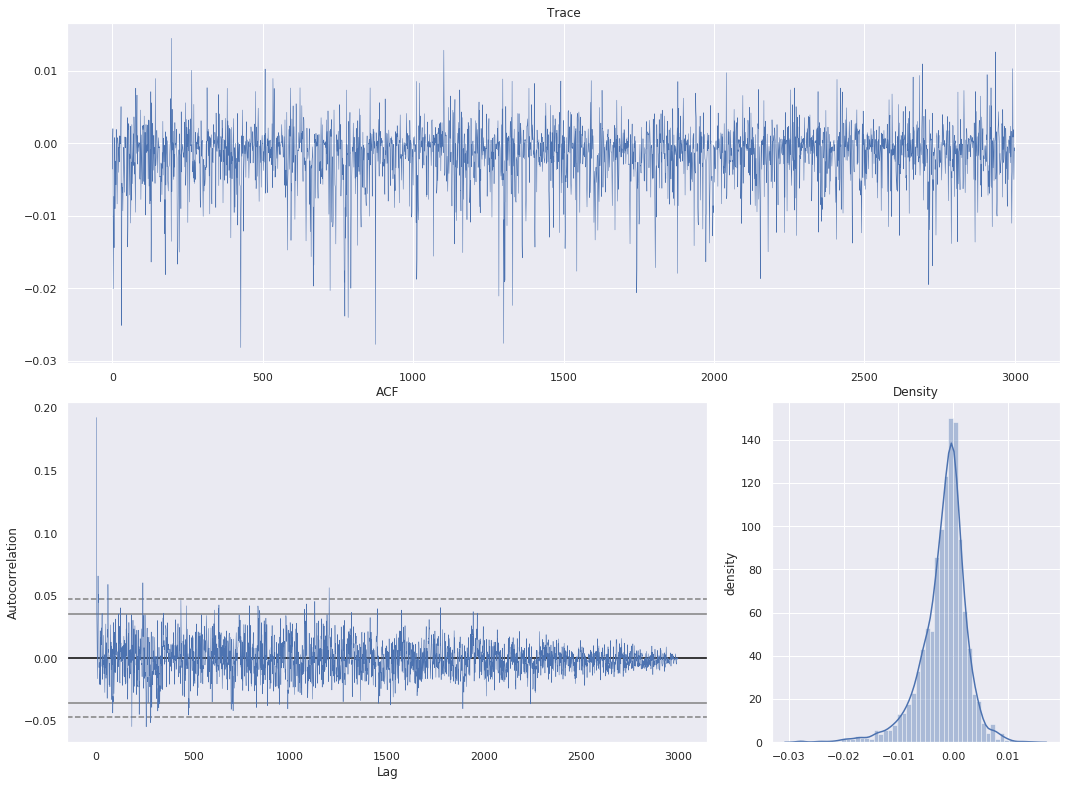
\includegraphics[width=0.8\linewidth]{diag_GIBBS_l400}
	}
	\subfloat{
		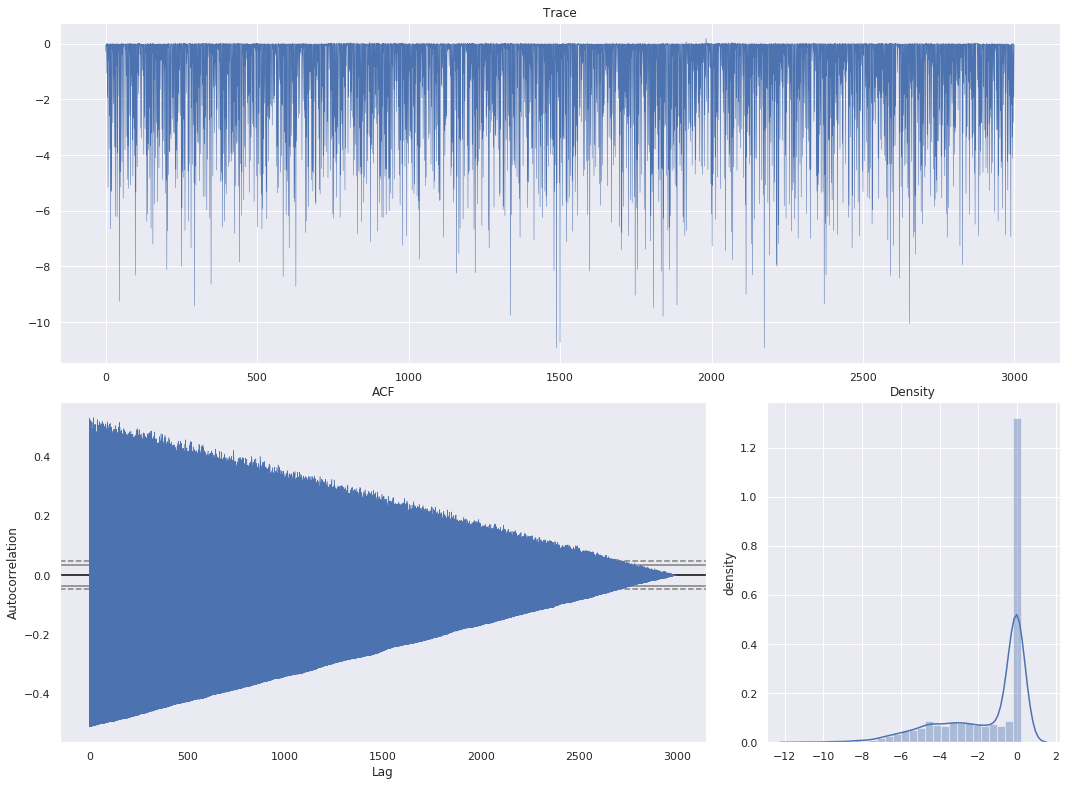
\includegraphics[width=0.8\textwidth]{diag_GIBBS_l1}
	}
	
	\caption{MCMC Diagnostics: BMB with a $\lambda$ of 400 (top) and 1 (bottom)}
	for the posterior marginal $(\Wxy)_{14}$.
	\label{fig:diag_GIBBS_l1_400}
\end{figure}

\FloatBarrier
\subsection{Modality of the Posterior}
\label{ss:modality}
In Chapter 3 we already mentioned that the modality of the posterior is important to consider when choosing an estimation method.
Additionally, the results of the previous section indicated that the posterior marginals of the individual $\Wxy$ edges get bimodal for very low $\lambda$. 
Instead of individual edges, we now look at the marginal posterior $ p(\Wxy|\matr{S}, \lambda)$ \footnote{$p(\Wxy | \matr{S}, \lambda)$ has shown to behave similarly to $p(\Wxy | \hat{S}, \lambda)$ for the Gibbs sampler, presumably because the copula does not have a big influence on Gaussian test data.}.
For this, linear \gls{PCA} was applied to reduce the dimensionality of the posterior.
The empirical distribution can then be observed alongside the first principal components.

In \autoref{fig:unimodality_art300}
the empirical posterior marginal of $\Wxy$ for one artificial data set is shown alongside the first principal components for $\lambda=300$.
%%%%%%%%%%%%%%% one mode artificial data
\begin{figure}[H]
	\centering
	\subfloat{
		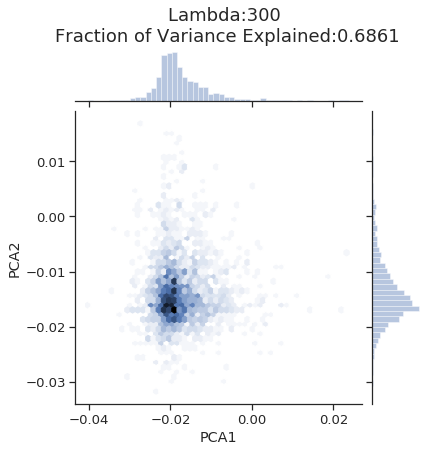
\includegraphics[width=0.48\linewidth]{PCA_W12_art_l300}
	}
	\subfloat{
		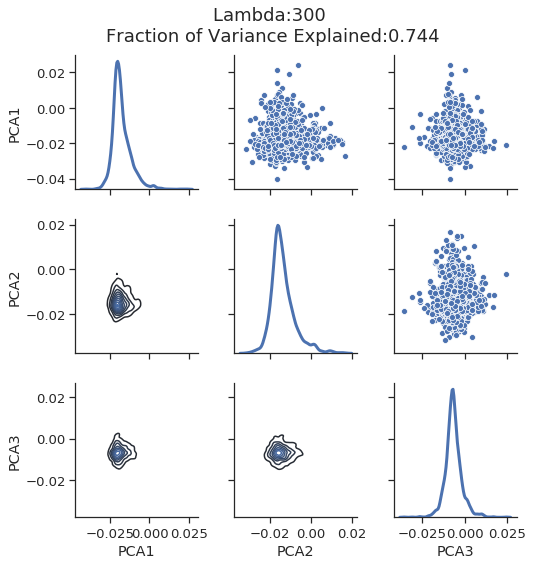
\includegraphics[width=0.48\linewidth]{PCA_W12_art_l300_2}
	}
	\caption{Empirical distribution of the $\Wxy$ posterior marginal over the first principal components for one example data set with $\lambda=300$.}
	
	\label{fig:unimodality_art300}
\end{figure}
It can be seen that the posterior is unimodal with a lot of mass surrounding the mode.
In contrast, a slightly lower $\lambda$ of $200$ already gets bimodal, as shown in \autoref{fig:unimodality_art200}.
%%%%%%%%%%%%%% multiple modes artificial data
\begin{figure}[H]
	\centering
	\subfloat{
		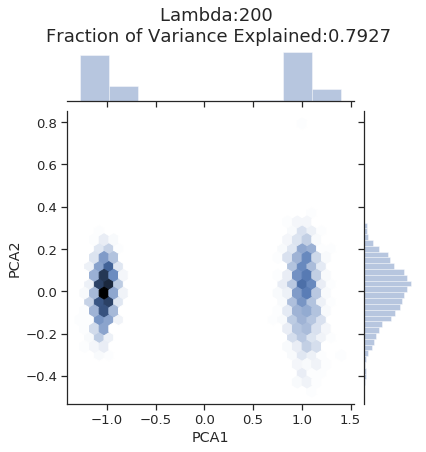
\includegraphics[width=0.48\linewidth]{PCA_W12_art_l200}
	}
	\subfloat{
		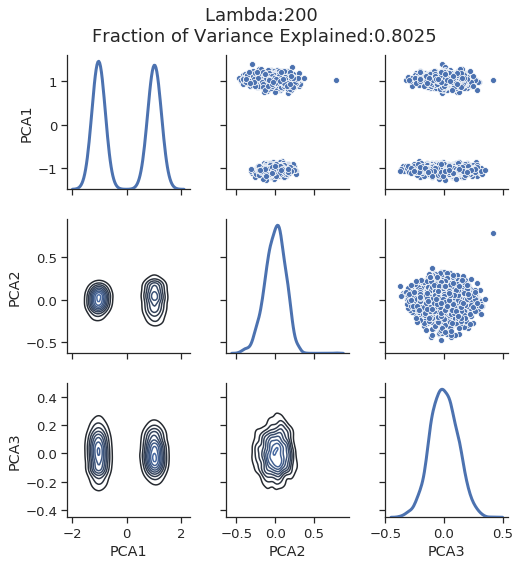
\includegraphics[width=0.48\linewidth]{PCA_W12_art_l200_2}
	}
	\caption{Empirical distribution of the $\Wxy$ posterior marginal over the first principal components for one example data set with $\lambda=200$.}
	
	\label{fig:unimodality_art200}
\end{figure}
Additionally, the distribution seems flatter alongside the first principal component. 
The corresponding MCMC diagnostics do not indicate any issues with the convergence in this range of $\lambda$.
%TODO show MCMC diag of lambda 200
As far as can be ascertained, the posterior stays unimodal for higher $\lambda$ and multi-modal for lower ones.
This change of modality aligns to the sudden change of sparsity of the Annealing in \autoref{fig:sparsitybylambda},
confirming that the fluctuation is indeed between two modes and not a result of numerical instability or bad mixing of the chain.
Consequently we can assume that the posterior distribution of $\Wxy$ actually is multi-modal for low $\lambda$.

An other interesting observation is that the variance explained by the first few principal components decreases for higher $\lambda$.
This could be due to the regularizing effect of the $\lambda$.
Aside from enforcing sparsity, the prior also decreases the values of the non-zero edges significantly.
If variance in the non-zero edges decreases faster than the variance of the zero-edges  (in terms of absolute values), the variance in the distribution is not anymore dominated by the non-zero edges.
This is illustrated in \autoref{fig:pca123}, where the distribution of a (truly) non-zero edge is compared to a zero edge
for a specific data set. 
Initially, the variance of the non-zero dominates and the PCA would still be able to a lot of information with just one axis. For higher $\lambda$ however, this changes and the joint distribution becomes more circular,
leaving a linear PCA no possibility to summarize the data in a low-dimensional projection (in this case onto one axis).
For higher dimensional data the behavior should be similar, with the joint distribution tending towards a sphere.

\begin{figure}
	\centering
	\subfloat{
		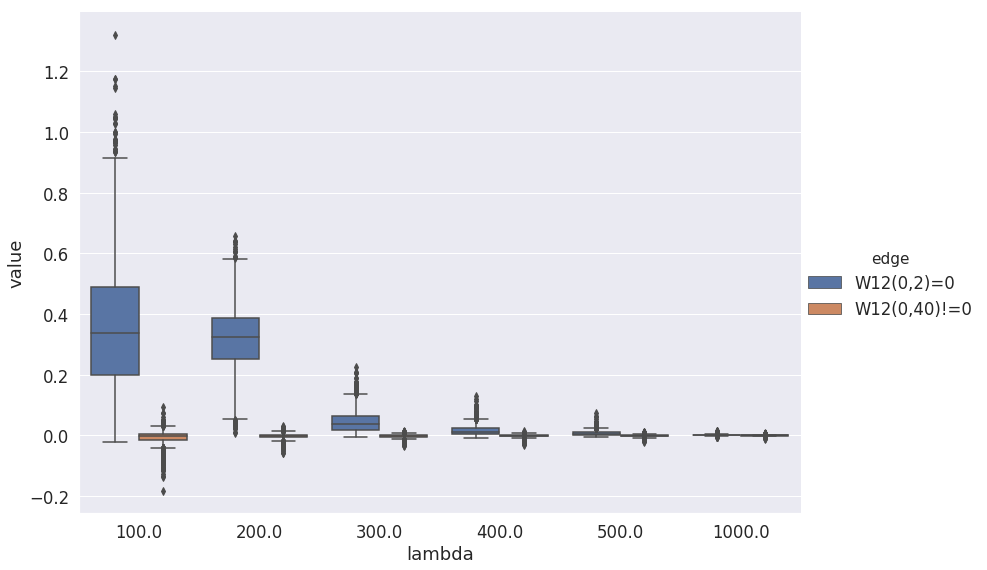
\includegraphics[width=0.8\textwidth]{pca_boxplot}
	}
	\qquad\qquad\qquad\qquad\qquad\qquad\qquad\qquad\qquad \\
	\subfloat{
		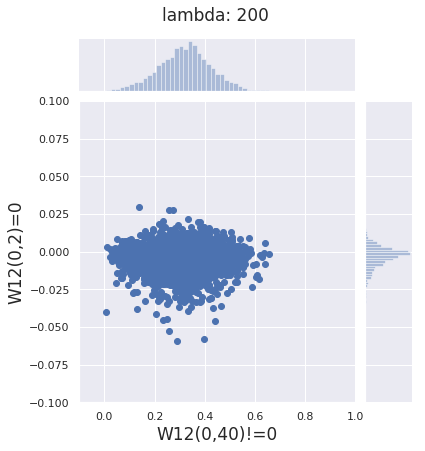
\includegraphics[width=0.31\textwidth]{pca1}
	}
	\subfloat{
		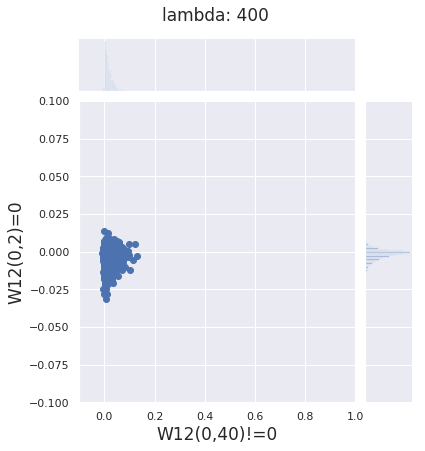
\includegraphics[width=0.31\textwidth]{pca2}
	}
	\subfloat{
		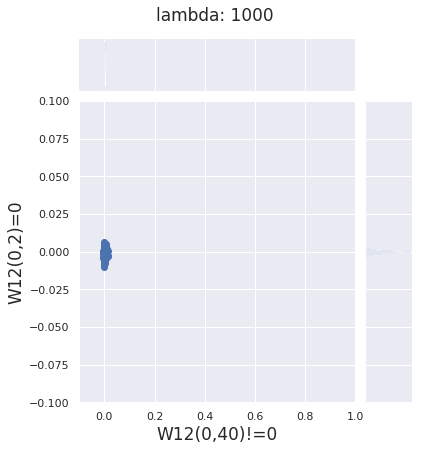
\includegraphics[width=0.31\textwidth]{pca3}
	}
	\caption{The effect of a higher $\lambda$ on the joint distribution between two marginals of the $\Wxy$ block. The true edge of $(\Wxy)_{(0,40)}$ (x-axis) is non-zero, while the true edge of $(\Wxy)_{(0,2)}$ (y-axis) is zero.}
	\label{fig:pca123}
\end{figure}


We now know the modality of $p(\Wxy | \lambda)$, but Simulated Annealing estimates the MAP of the joint posterior $p(\Wxx, \Wxy, \matr{T} | \hat{S}, \lambda)$.
Unfortunately we are unable infer anything significant about the joint posterior because the first few (2-3) principal components only explain a low amount of the variance ($<10\%"$), rendering the 2 dimensional projection useless.





\subsection{Quality of Reconstructed Networks}
\label{ss:quality}
With the range of possible $\lambda$ established, the predictive performance of the individual methods can be analyzed.

The performance metrics for the \gls{BMB}, GLASSO and \gls{SA} are visualized in \autoref{fig:metrics_BMB}.
We plotted the mean over all datasets as well as error bars corresponding to a $95\%$ bootstrapping confidence interval for the mean.
\begin{figure}
	\centering
	\subfloat{
		\makebox[\textwidth][c]{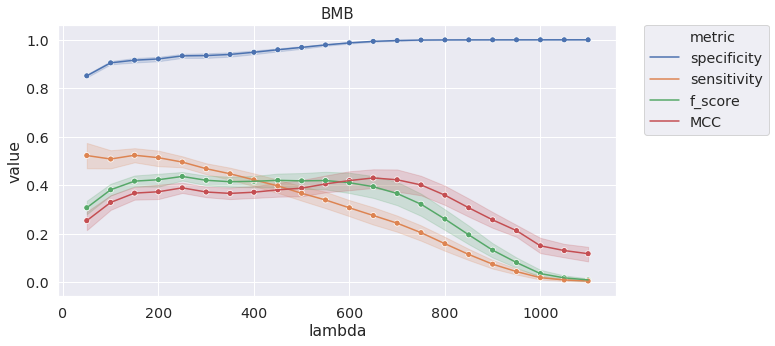
\includegraphics[width=1.05\textwidth]{metrics_BMB}}%
	}
	\subfloat{
		\makebox[\textwidth][c]{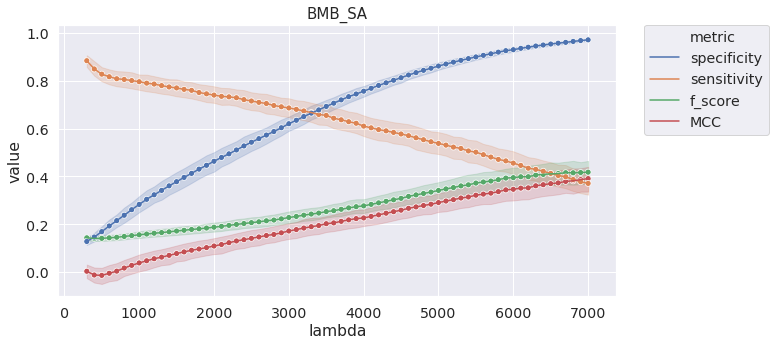
\includegraphics[width=1.05\textwidth]{metrics_SA}}%
	}
	\subfloat{
		\makebox[\textwidth][c]{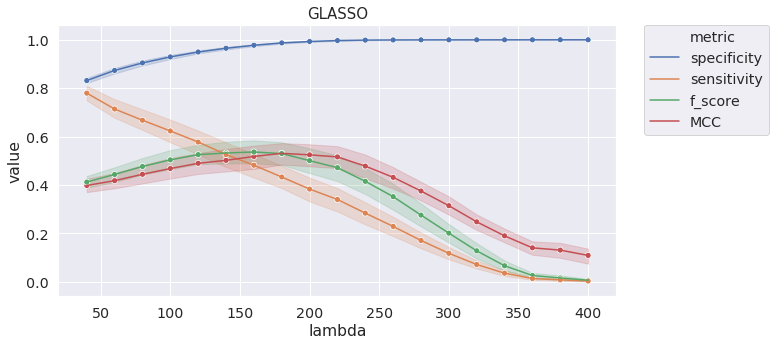
\includegraphics[width=1.05\textwidth]{metrics_GLASSO}}%
	}
	\caption{Average performance metrics for the Gibbs BMB, Simulated Annealing, and the GLASSO.
		The shaded area corresponds to a 95\% bootstrapping confidence interval for the mean.}
	\label{fig:metrics_BMB}
\end{figure}
First of all, the effect of the $\lambda$ on the specificity is of interest.
It can be seen that the specificity generally increases with a higher $\lambda$ for all three methods, which is to be expected due to its sparsity inducing property.
Furthermore, there is a linear relationship between the fraction of nonzero edges and the specificity, as shown in \autoref{fig:sparsity_vs_specificity}.
In practical applications we can only observe the resulting network, so this relation is very useful.
We can effectively control for the specificity by adjusting $\lambda$ until a satisfactory density of the network graph is reached.
\begin{figure}
	\centering
	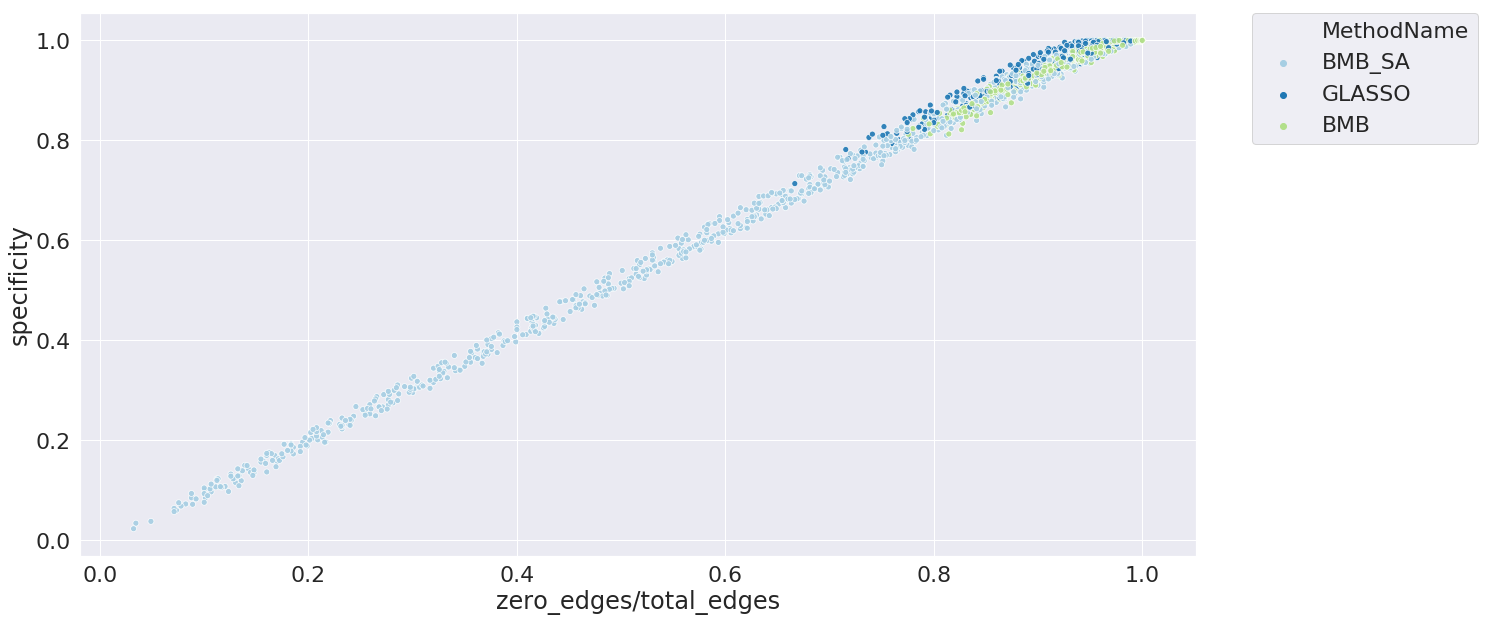
\includegraphics[width=0.9\textwidth]{sparsity_vs_specificity}
	\caption{Relation between the sparsity in the reconstructed networks and the resulting specificity for all 40 data sets.}
	\label{fig:sparsity_vs_specificity}
\end{figure}
While the BMB and GLASSO show a maximum average MCC and F-score at around 600 and 200 respectively, the limited range of the Annealing seems to not include it's maximum.
But the drop in sensitivity for very high $\lambda$ will also have to occur in the Annealing as the networks will presumably be empty for a high enough $\lambda$.
With the specificity already getting close to 1, we can thus assume that we would not observe much of an improvement for slightly higher $\lambda$.
Nonetheless, the Annealing reaches values of around 0.4 for both the F-Score and the MCC, which are comparable to the performance of the BMB.
But in all cases, the SA and BMB are outperformed by the GLASSO.
Aside from that, the Annealing is capable of covering a wider range of the sensitivity, allowing the estimation of less sparse networks.

To show the similarity between the methods, we fix $\lambda$ such that the resulting network size for the test data is (close to) equal in all methods.
In \autoref{fig:boxplot_metrics_fixlambda}  the performance for individual data sets is shown for these fixed $\lambda$. 
While the GLASSO always has the highest MCC and F-score, the difference between the Annealing and the BMB is not that well-defined.
In addition, the methods mostly agree on the relative performance for the specific data sets.
For example, all show low performance on data sets 160 and 180 while performing well on 178.
%%%%%%%%% for each dataset with fixed lambda
\begin{figure}
	\centering
	\subfloat{
		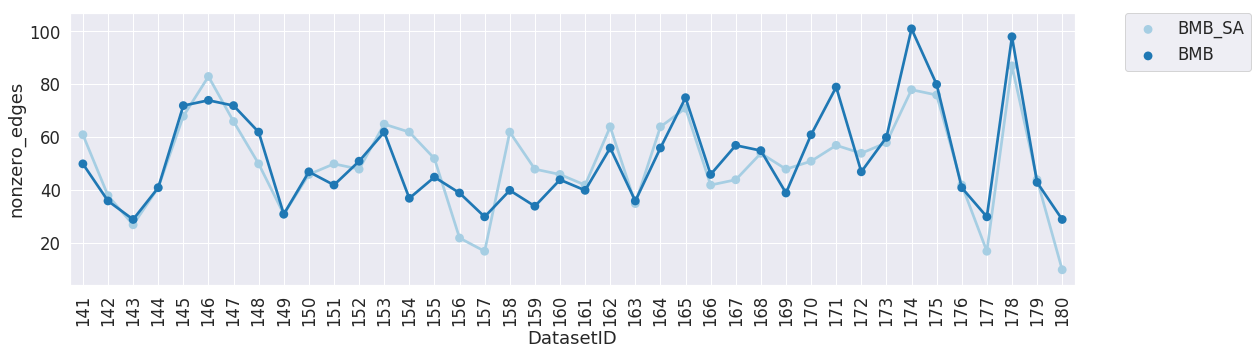
\includegraphics[width=\linewidth]{fixlambda_sparsity}
	}
	\subfloat{
		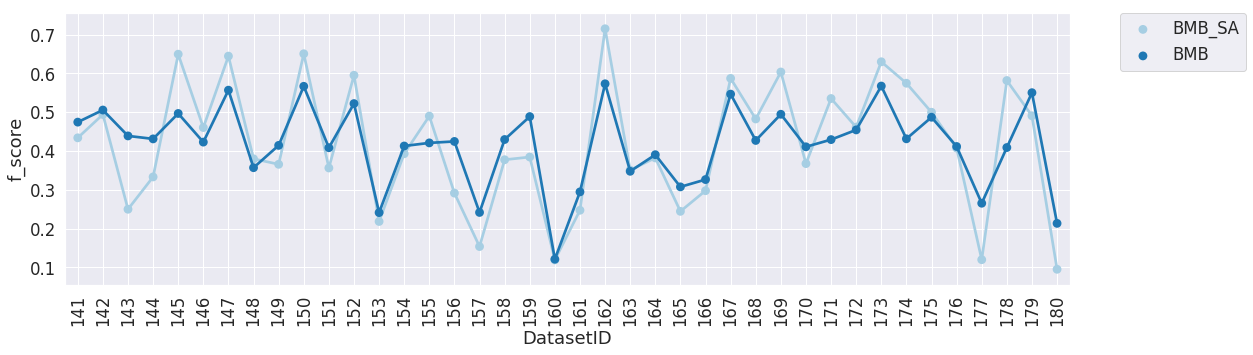
\includegraphics[width=\linewidth]{fixlambda_fscore}
	}
	\subfloat{
		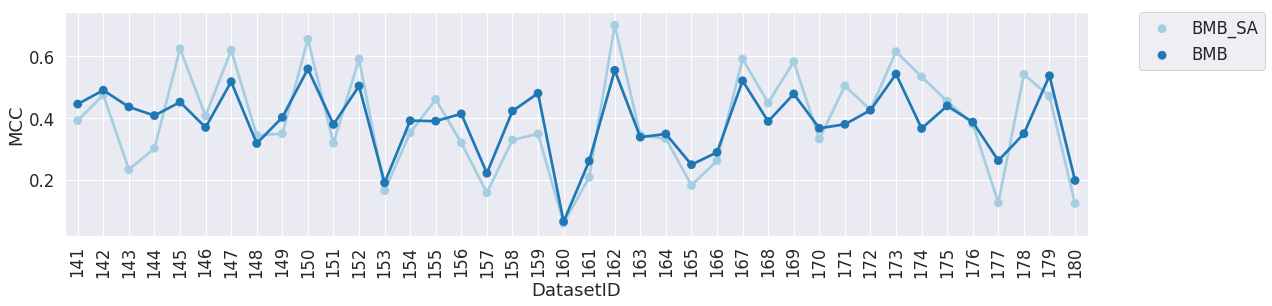
\includegraphics[width=\linewidth]{fixlambda_MCC}
	}
	\caption{Different Metrics for fixed $\lambda$ resulting in a roughly similar network size.}
	\label{fig:fix_lambda_bydataset}
	$\lambda_{BMB}=500 \quad$
	$\lambda_{SA}=7000\quad$
	$\lambda_{GLASSO}=150$
\end{figure}
Aside from confirming the previous results, the box-plots in \autoref{fig:fix_lambda_bydataset} furthermore show that the Annealing exhibits a higher variance among different data sets than the BMB for basically all metrics, excluding the specificity (with fixed $\lambda$).

%%%%%%%%%%%%%%%% boxplots fixed lambda
\begin{figure}
	\centering
	\subfloat{
		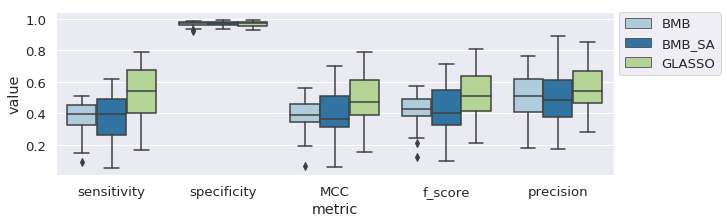
\includegraphics[width=0.9\linewidth]{boxplot_metrics_fixlambda}
	}
	\subfloat{
		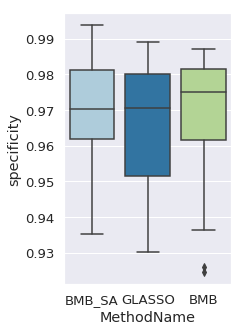
\includegraphics[width=0.25\linewidth]{boxplot_metrics_fixlambda_spec}
	}
	\caption{Different Metrics for fixed $\lambda$ resulting in an approximately similar network size.}
	\label{fig:boxplot_metrics_fixlambda}
	$\lambda_{BMB}=500 \quad$
	$\lambda_{SA}=7000\quad$
	$\lambda_{GLASSO}=150$
\end{figure}

Finally, we will look at how the performance of the methods relate to the sparsity for easing the search of a suitable $\lambda$ in practice.
While information criteria such as the (extended) BIC \citep{foygel2010extended} are popular for model selection of \gls{GGM}s, they are based on the calculation of the (log) likelihood, which requires the complete matrix $\W$.
In our current setting for the Simulated Annealing,
the whole precision matrix is not available since cooling the $\Wyys$ block would change the estimated joint MAP (see \autoref{ss:joint_map}).
Consequently we have to look at networks resulting from a range of different $\lambda$ and see how they change for different $\lambda$.
In this case, knowing how the model generally behaves in relation to the sparsity can then be helpful.
\autoref{fig:hexbin} shows the relation between the number of zero-edges and the metrics.
We can see that both the F-Score and the MCC are highest when in the range corresponding to the true sparsity of the networks (which is between around $90\%$ to $94.\overline{4}\%$).
After reaching this point, the sensitivity drops sharply for sparser graphs while the specificity only increases slowly,
thus resulting in a decrease of the F-score and MCC.
However, even for higher sparsity the specificity does not always reach $100\%$ for non-trivial graphs.
So for avoiding false positives it is advisable to overestimate the sparsity of the target network when selecting a $\lambda$.
Aside from that, the plots agree with the previous results in relation to the $\lambda$.

%%%%%%%%%%%%%%% sparsity vs others, hexbin with polynomial regression
\begin{figure}
	\centering
	\subfloat{
		\makebox[\textwidth][c]{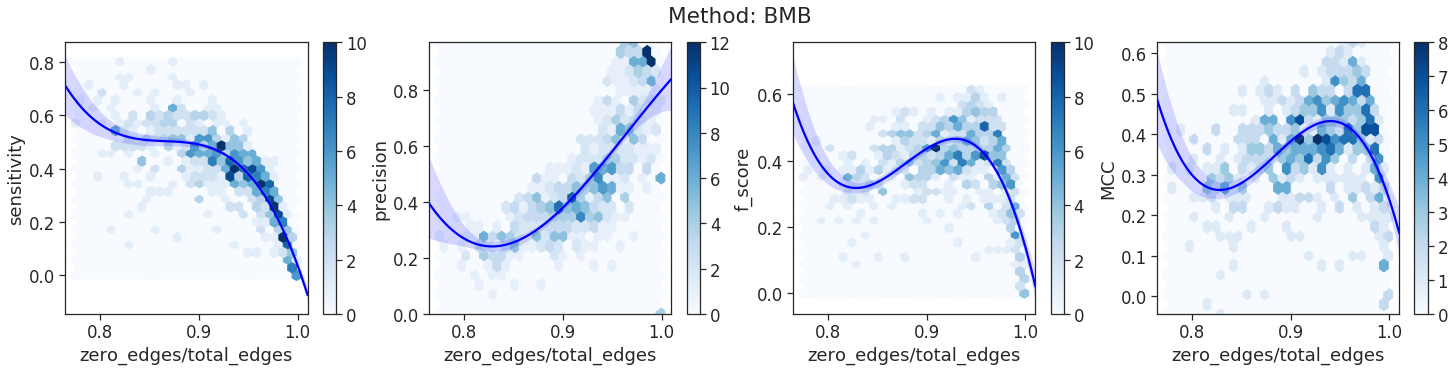
\includegraphics[width=1.2\textwidth]{sparsity_vs_all_BMB}}%
	}
	\subfloat{
		\makebox[\textwidth][c]{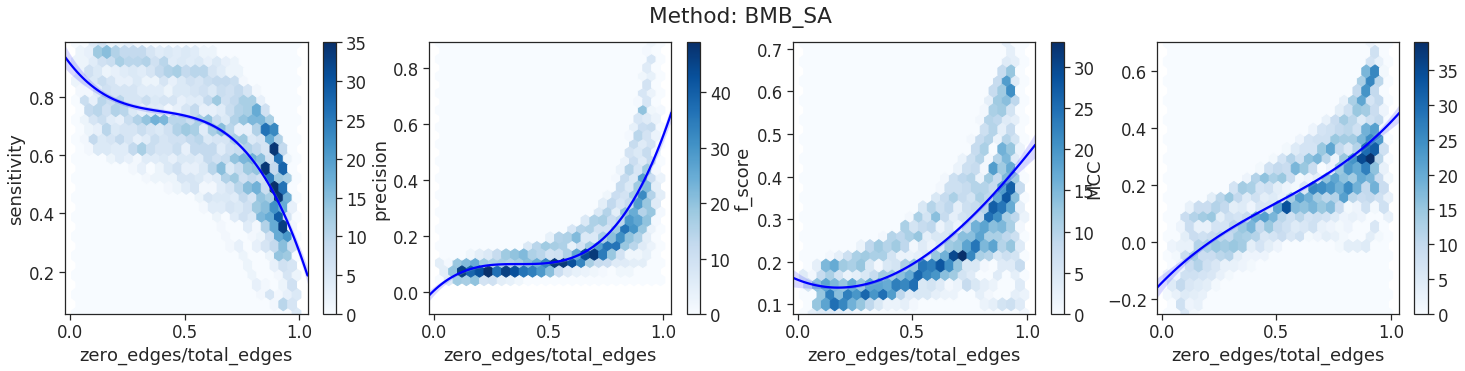
\includegraphics[width=1.2\textwidth]{sparsity_vs_all_BMB_SA}}%
	}
	\subfloat{
		\makebox[\textwidth][c]{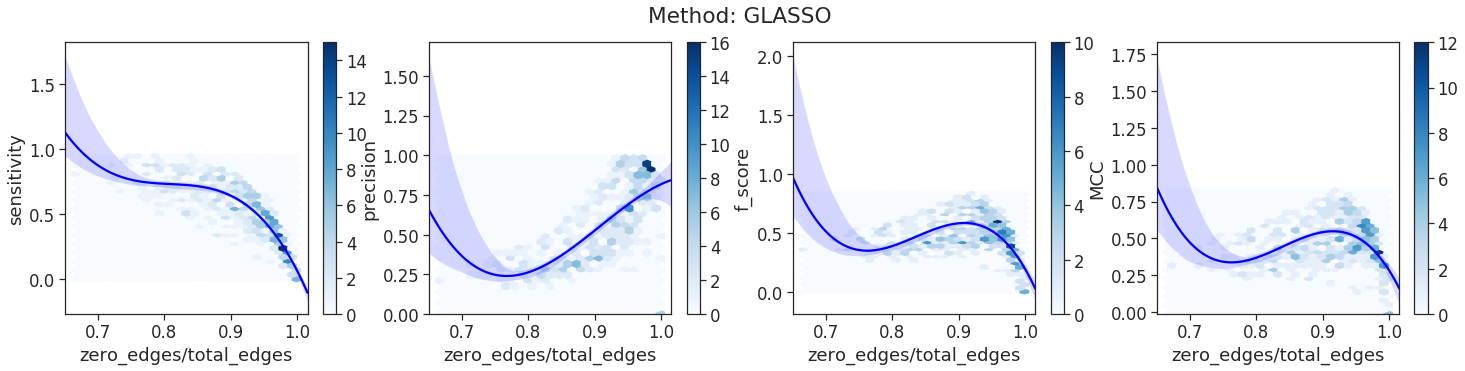
\includegraphics[width=1.2\textwidth]{sparsity_vs_all_GLASSO}}%
	}
	\caption{Relationship between the sparsity of the reconstructed Network and different performance measurements.
		The plots were created using 2D histograms with hexagon binning and a polynomial regression of degree 3.}
	\label{fig:hexbin}
\end{figure}
\FloatBarrier

The similarity of the resulting networks for the BMB and SA is illustrated in \autoref{fig:graph_BMB_MCC} and \autoref{fig:graph_SA_MCC}.
While they still slightly differ, we could not find any consistent advantage in either of them (in terms of the used measures).
More sophisticated graph comparison methods would be necessary for a better understanding of their actual differences.
Attempts at combining the two methods by intersection of the resulting graphs has proven to be difficult due to the different scales of $\lambda$.
Even when parameters resulting in the same network size were found, the combinations did not provide any significant improvement.
\begin{figure}
	\centering
	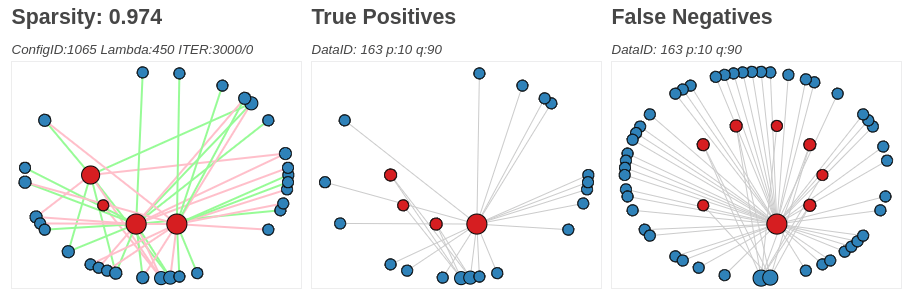
\includegraphics[width=1\linewidth]{graph_BMB_0974}
	\caption{W12 subnetwork reconstructed with Gibbs BMB (for artificial data with id 162)}
	\label{fig:graph_BMB_MCC}
\end{figure}
\begin{figure}
	\centering
	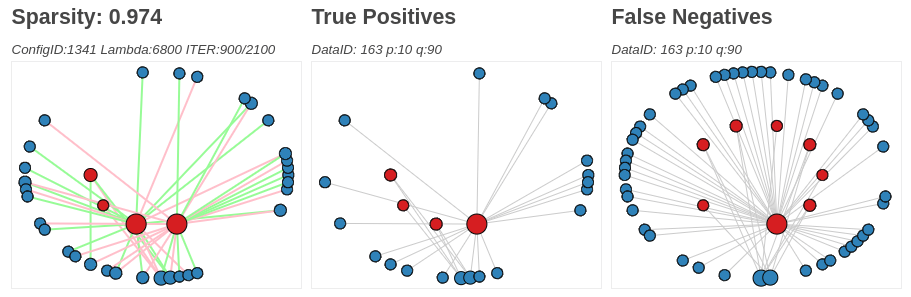
\includegraphics[width=1\linewidth]{graph_SA_0974}
	\caption{W12 subnetwork reconstructed with SA (for artificial data with id 162)}
	\label{fig:graph_SA_MCC}
\end{figure}


\FloatBarrier
\section{Application on Real Data: HIV-X}
We now switch to the Markov Blanket estimation in context of the HIV-X MRD Project \citep{HIVX}.

The \gls{HIV} is one of the most widespread and harmful viruses in the world.
If left untreated, it leads to the reduction of T helper cells expressing CD4, which are essential for the immune system.
The final stage of the infection is accompanied by a complete shut down of the immune system and is referred to as \gls{AIDS} (e.g. \cite{alimonti2003mechanisms}). 
Lacking a working immune system, affected individuals become vulnerable to opportunistic diseases such as toxoplasmosis and pneumonia, which may ultimately lead to death \citep{chaisson1998impact}.
While current treatments are effective at suppressing the virus by targeting stages of its life-cycle \citep{bartlett2001overview}, no cure that completely eliminates the virus has yet been found.
Even when the virus is suppressed by treatment, latent HIV reservoirs remain ineradicable and ready to multiply as soon as treatment is stopped.
Another ongoing problem of HIV treatment is the high mutation rate of the virus; 
mutations can lead to resistances against specific antiretroviral drugs (and even multiple drugs) in the patient, rendering treatment with those drugs ineffective \citep{wainberg1998public}.
Once developed, such resistances reduce the potency of the relevant drugs for a lifetime \citep{noe2005latent}.
The swiss HIV-X MRD Project \citep{HIVX} aims to identify factors in latent viral reservoirs pertinent to the future treatment of patients.
Using the Markov Blanket estimation we investigate HIV-1 data available from the HIV-X Project
for potential interactions significant to the therapy of patients.
Among others, this includes the interactions between resistance relevant mutations and multiple clinical factors such as the viral load.

\subsection{Data and Setup}
The data of the HIV-X MRD Project \citep{HIVX} is a subset of the Swiss HIV Cohort Study \citep{SHCS}, consisting only of treatment experienced HIV-1 patients.
That is, all individuals have been successfully treated with \gls{ART} for at least five years.
This implies that the viral load has been suppressed to non-detectable levels and the measured RNA levels of HIV in the data mostly remain very low.
The exceptions are occasional so-called 'blips'.
A blip is a transient but measurable spike of the viral load,
in patients for whom the virus is effectively suppressed to undetectable levels.
The significance of blips has not yet been established and remains controversial.
While some studies found associations with the development of drug resistances \citep{stuart2001transient} and the CD4 cell count recovery \citep{martinez2005hiv}, others claim blips to be of limited significance \citep{lee2006hiv}.

Aside from the viral load measured by RNA levels in the plasma, the data contains CD4 and CD8 cell counts.
CD8 T cells are an important part of the immune system and are responsible for controlling HIV in the early infection phase \citep{gulzar2004cd8}.
While an infection initially leads to an increase in CD8 T cell count, they decrease again in later stages \citep{roederer1995cd8}.
Furthermore, a quantification of the HIV DNA obtained by \gls{ddPCR} is provided, as viral load is undetectable for all the patients.
Droplet Digital PCR is a method for accurately measuring the DNA copy number, and has since recently been applied in the context of HIV \citep{strain2013highly}.
Additionally, two differently obtained sets of resistance relevant mutations of the patients are available.
The first one is based on Genomic Resistance Testing (GRT).
Even though resistances mostly arise in response to \gls{ART},
they may also be transmitted to newly infected individuals.
As this should be taken into account when choosing a treatment,
new patients as well as patients experiencing treatment failure are subject to \gls{GRT} \citep{shafer2002genotypic, huldrych_antiretroviralrecomm}.
The second set of resistance relevant mutations is based on haplotype
reconstruction of \gls{NGS} data.
The gag-pol region of the viral genome was reconstructed with
PredictHaplo\footnote{Source of PredictHaplo: \href{https://bmda.dmi.unibas.ch/software.html}{https://bmda.dmi.unibas.ch/software.html}}\citep{prabhakaran2014hiv}. Subsequently the reconstructed haplotypes were translated
into (possible) amino acids.
With the amino acids of the haplotypes available, resistance relevant mutations were mapped according to the '2017 Update of the Drug Resistance Mutations in HIV-1' \citep{shafer2017human}.

An overview of the variables available for each individual patient is shown in the following table.
The first $p=5$ variables are query variables for which we wish to infer dependencies; the remaining $q=225$ variables pertain to resistance relevant mutations, and the drugs used in the treatments.
\begin{table}[H]
	\begin{tabular}{lcl}
		\textbf{Variable} & \textbf{Domain}      & \textbf{Description}                                                 
		\\
		\toprule
		CD4               & $\mathbb{R}_{\geq0}$ & CD4 T cell count                                                     \\
		CD8               & $\mathbb{R}_{\geq0}$ & CD8 T cell count                                                     \\
		RNA               & $\mathbb{R}_{\geq0}$ & Viral Load / HIV RNA Level                                           \\
		HIV\_copies       & $\mathbb{R}_{\geq0}$ & Measured by HIV DNA cell count with ddPCR                            \\
		SLOPE\_ddPCR      & $\mathbb{R}$         & Error corrected change of HIV\_copies to next time point             \\
		\midrule
		HIST\_DRU\_*      & $\{0,1\}^{34}$         & Administered ART drugs in any previous treatment               
		\\
		&                      & (e.g. HIST\_DRU\_EFV for Enfuvirtide                                 
		\footnote{\href{https://aidsinfo.nih.gov/drugs/306/enfuvirtide/0/patient}{https://aidsinfo.nih.gov/drugs/306/enfuvirtide/0/patient}})
		\\
		drug*            & $\mathbb{N}^{34}$         & Amount of days the drug has been administered in current treatment.
		\\&& Is 0, if the patient is currently not taking this drug 
		\\&&(e.g. drugEFV)                          
		\\
		MU\_*             & $\{0,1\}^{77}$         & Resistance relevant mutations obtained with \gls{GRT}
		\\
		&                      & (e.g. MU\_RT103)                                                     \\
		INT*/PR*/RT*      & $\{0,1\}^{80}$         & Resistance relevant mutations inferred from 
		\\
		&                      & reconstructed haplotypes (e.g. RT103)                                                         
	\end{tabular}
\end{table}

Tests for CD4/8 counts, viral load and ddPCR did (mostly) not occur at the same time.
As the ddPCR offers the most reliable estimate of HIV persistence in successfully treated patients,
the data has been merged such that each sample corresponds to one of a patient's ddPCR measurements;
for each patient, there are between 2 to 5 such measurements available, each from a different point in time.
Viral load and CD4/8 cell counts in each sample correspond to the measurements closest in time to the respective ddPCR value.
Additionally, the rate of change between successive (patient-wise) ddPCR measurements is included as $SLOPE\_ddPCR$.

In total there are 2760 samples with 1092 individual patients.
For 268 individuals, resistance mutations from the haplotype reconstruction are available.
In contrast to that, the GRT mutations as well as the prior and current treatments are available for all patients.
A short summary of the variables of interest is given in \autoref{table:summaryHIV}.
\begin{table}[H]
	\centering
	\caption{Summary of the (non-boolean ) variables in the data set.}
	\label{table:summaryHIV}
	
	\makebox[\linewidth]{
	\begin{tabular}{lrrrrrr}
		\toprule
		{} &      CD4 &      CD8 &       RNA &  SLOPE\_ddPCR &  HIV\_copies &  days\_since\_1stddPCR \\
		\midrule
		\textbf{count} &  2760.00 &  2754.00 &   2734.00 &      2760.00 &     2760.00 &              2760.00 \\
		\textbf{mean } &   524.96 &   823.92 &     54.15 &        -0.02 &     4111.24 &               643.03 \\
		\textbf{std  } &   256.10 &   393.13 &   1155.23 &        27.67 &   104741.81 &               697.02 \\
		\textbf{min  } &     0.00 &     0.00 &      0.00 &      -585.95 &        0.00 &                 0.00 \\
		\textbf{25\%  } &   345.00 &   547.00 &      0.00 &        -0.01 &      215.49 &                 0.00 \\
		\textbf{50\%  } &   484.00 &   755.00 &      0.00 &         0.00 &      448.94 &               693.00 \\
		\textbf{75\%  } &   663.00 &  1019.50 &      0.00 &         0.03 &      861.78 &               875.00 \\
		\textbf{max  } &  2101.00 &  3407.00 &  39178.00 &       899.29 &  4238988.63 &              5249.00 \\
		\bottomrule
	\end{tabular}
	}
\end{table}
As expected for successfully treated patients, the viral load is small for most of the data, except for the occasional blips.
This is also illustrated in \autoref{fig:blipsdist}.
The ddPCR in \textit{HIV\_copies} and the corresponding slopes furthermore exhibit a few extreme outliers,
which can also be seen in \autoref{fig:ddPCRdist}.
The outliers should not be problematic for the estimation, since the extended likelihood of the copula depends only on an order preserving statistic.
\begin{figure}[h]
	\centering
	\subfloat{
		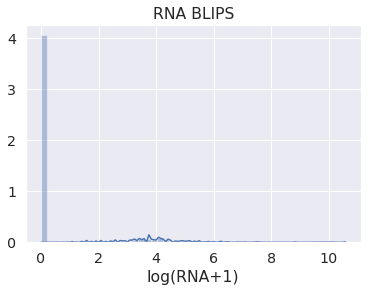
\includegraphics[width=0.45\linewidth]{HIV_distplot_blips}
	}
	\subfloat{
		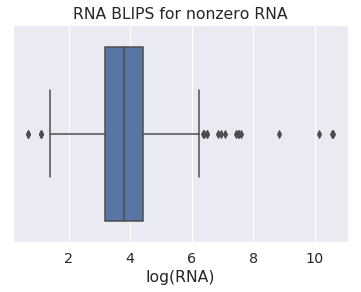
\includegraphics[width=0.45\linewidth]{HIV_histplot_blips_nonzero}
	}
	\caption{Distribution of the viral loads. The Boxplot only includes the non-zero values.}
	
	\label{fig:blipsdist}
\end{figure}
\begin{figure}[h]
	\centering
	\subfloat{
		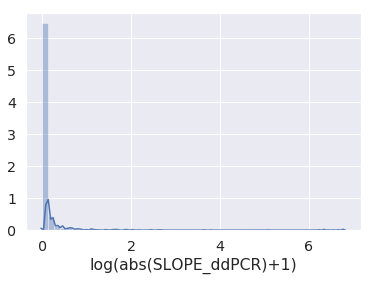
\includegraphics[width=0.48\linewidth]{HIV_distplot_slopelog}
	}
	\subfloat{
		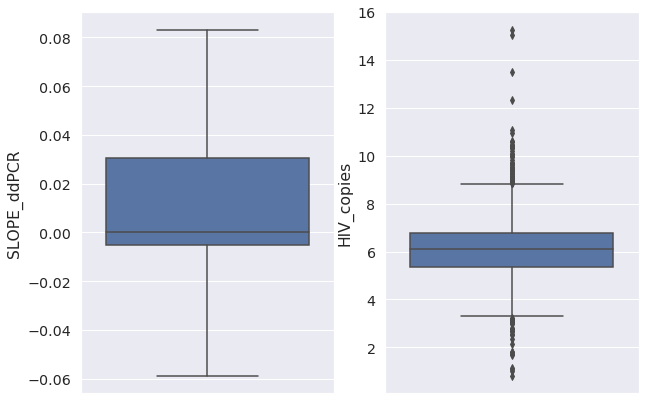
\includegraphics[width=0.48\linewidth]{HIV_histplot_ddPCR}
	}
	\caption{Distribution of ddPCR HIV\_copies and ddPCR slope.}
	
	\label{fig:ddPCRdist}
\end{figure}
In \autoref{fig:ngs_time_diff} the time difference between the NGS and the GRT data is given.
It can be seen that the majority of the GRT mutations are either from the same date as the NGS data (the start of the treatment) or a later point of time (presumably when treatment had to be switched).

The patients in the data set have been observed for up to 14 years (see \autoref{fig:days_since_1stddpcr}), while 
the NGS testing is only done once for each patient.
It would be questionable to assume that the haplotypes of the virus remain unchanged,
over such a long interval and during possibly multiple treatment changes.
For this reason we will only use the first sample of each patient for the network estimation,
as it is closest in time to the NGS data.
\begin{figure}
	\centering
	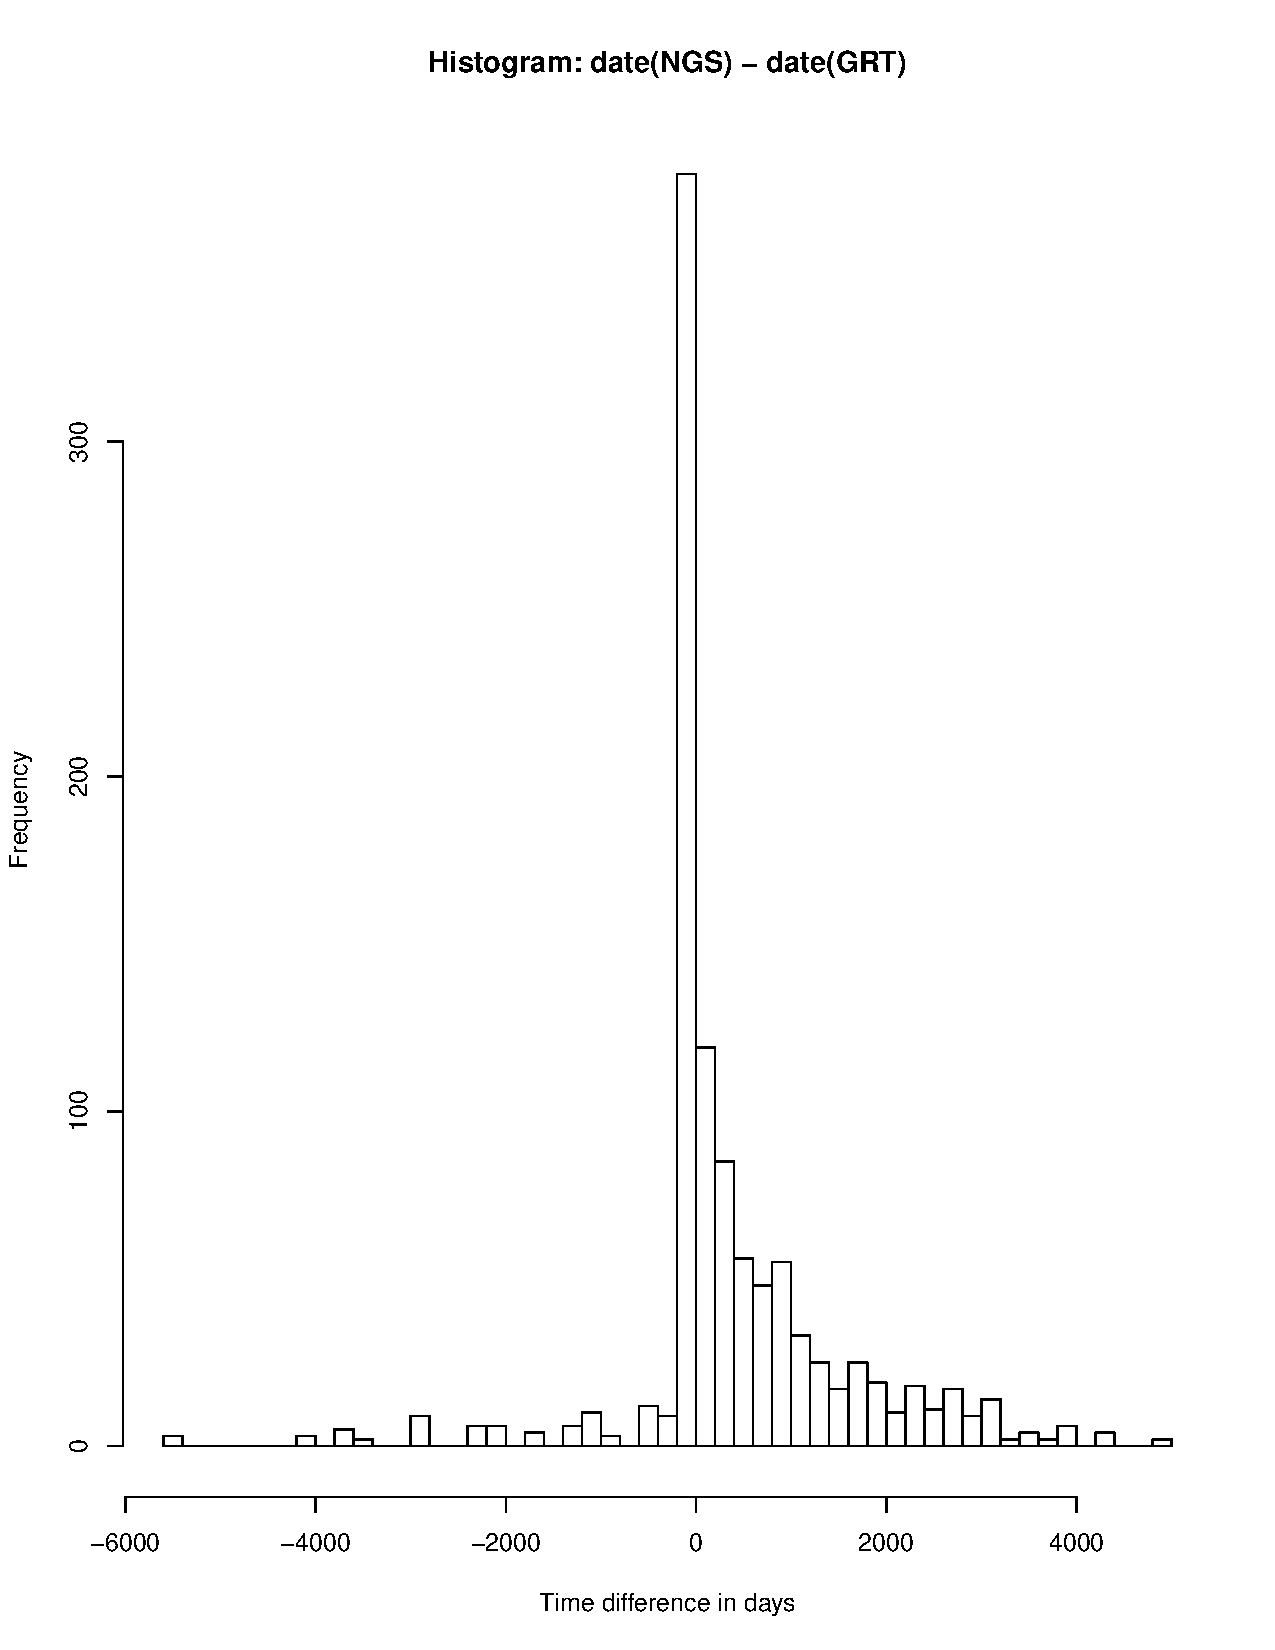
\includegraphics[page=1, width=0.7\textwidth]{NGS_vs_GRT_time}
	\caption{Histogram of patient wise time difference (in days) between the GRT mutations and the NGS data.}
	\label{fig:ngs_time_diff}
\end{figure}
\begin{figure}
	\centering
	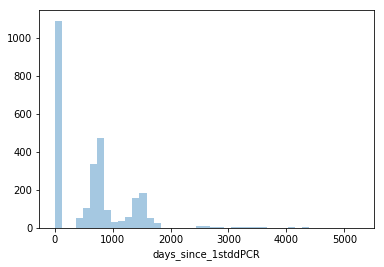
\includegraphics[width=0.6\textwidth]{days_since_1stddpcr}
	\caption{Histogram of time passed between current ddPCR sample and the first ddPCR test of the respective patient.}
	\label{fig:days_since_1stddpcr}
\end{figure}
\FloatBarrier
\ \ \\
\pagebreak
\subsubsection*{Setup}
The settings for the Gibbs BMB and the Annealing run are given in \autoref{table:settings_model_HIV}.
Note that in contrast to the test data setting, no thresholding Credible Interval was set in advance.
\begin{table}[H]
	\centering
	\caption{Model Parameters used for the HIV-X Data\label{table:settings_model_HIV}}
	\begin{tabular}{l c c}
		& \textbf{BMB}   & \textbf{Simulated Annealing} \\
		\toprule
		Total Iterations  & $7000$         & $7000$                       \\\midrule
		Gibbs Sweeps      & $7000$         & $2100$                        \\
		Burn-In           & $2100$          & $630$                        \\
		Cooling Steps     & -              & $4900$                       \\
		Draws at $T_n$    & -              & $490$                        \\
		$T_0$             & -              & $1$                          \\
		$T_n$             & -              & $0.01$                       
	\end{tabular}
\end{table}

% Data description
%% -> source
%% -> haplotype inferred mutations / genotype resistance testing mutations

\subsection{Modality of the Posterior}
Analogous to the test setting, we look at a low dimensional projection of the marginal posterior distribution $ p(\Wxy|\matr{Z}\in D, \lambda)$ 
via PCA.
As it turns out, the $\Wxy$ posterior appears to be multi-modal for $\lambda$ lower than 250,
while being unimodal for higher $\lambda$.
Figures \ref{fig:unimodality_HIV200} and \ref{fig:unimodality_HIV300} show the distributions for a $\lambda$ of 200 and 300 respectively.
It should be noted again that the first two principal components for $\lambda=300$ only explain about $32\%$ of the variance in the data,
so the projection is rather inaccurate.
Therefore the conclusion on unimodality should be taken with caution.
When looking at the MCMC diagnostics, we could not find any indications of convergence problems for $\lambda=200$, $\lambda=300$.
A representative example for the diagnostic plots is shown in \autoref{fig:diagnostics200} and \autoref{fig:diagnostics300}.
Both the autocorrelation and the trace plot seem acceptable.
In contrast, $\lambda$ of 50 and lower are to be avoided, as the autocorrelation indicate repeating fluctuation in the samples (see \autoref{fig:diagnostics50}).

But in general, the multi-modality for low $\lambda$ is not an unexpected observation.
A big part of the HIV data, namely the resistance mutations of the haplotypes and GRT, as well as current and previous treatments, are very sparse.
In addition, there are a lot of missing values for the haplotype mutations and the data is high dimensional ($230$ variables for $1092$ samples).
Therefore it is reasonable that various configurations are capable of explaining the data, if the prior does not enforce a lot of sparsity in the parameters.
As a consequence we will avoid the annealing in this $\lambda$ region.

%%%%%%%%%%%%%% multiple modes HIV data
\begin{figure}[H]
	\centering
	\subfloat{
		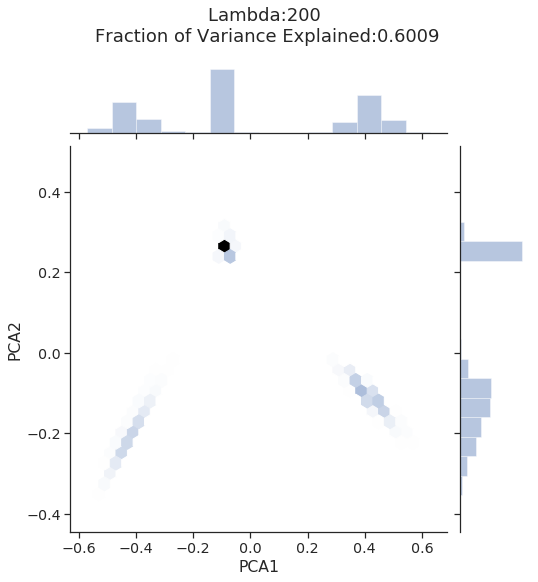
\includegraphics[width=0.48\linewidth]{PCA_W12_HIV_l200}
	}
	\subfloat{
		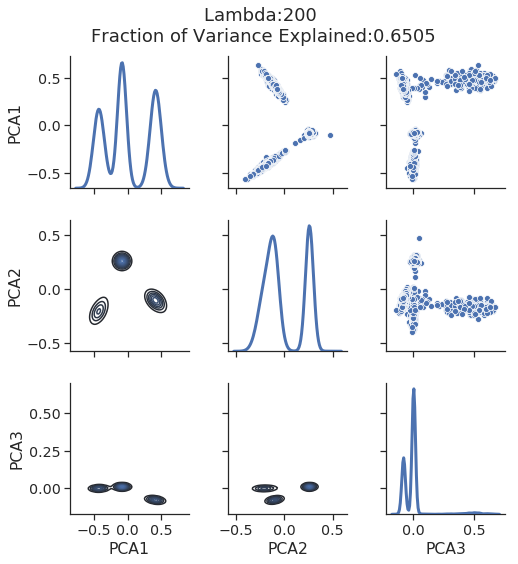
\includegraphics[width=0.48\linewidth]{PCA_W12_HIV_l200_2}
	}
	\caption{Empirical distribution of the $\Wxy$ posterior marginal over the first principal components with $\lambda=200$.}
	
	\label{fig:unimodality_HIV200}
\end{figure}
%%%%%%%%%%%%%%% one mode HIV data
\begin{figure}[H]
	\centering
	\subfloat{
		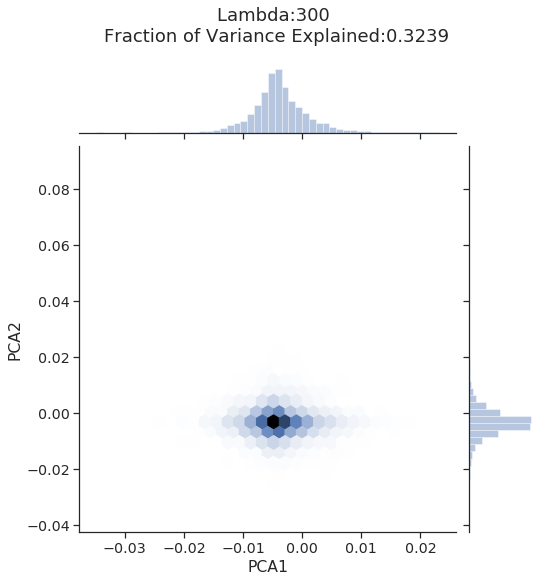
\includegraphics[width=0.48\linewidth]{PCA_W12_HIV_l300}
	}
	\subfloat{
		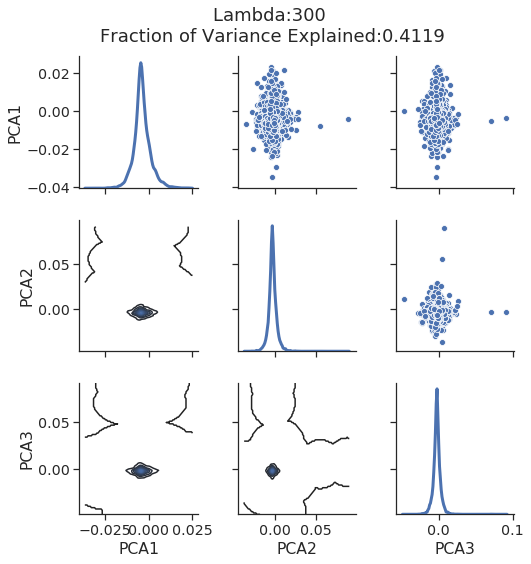
\includegraphics[width=0.48\linewidth]{PCA_W12_HIV_l300_2}
	}
	\caption{Empirical distribution of the $\Wxy$ posterior marginal over the first principal components with $\lambda=300$.}
	
	\label{fig:unimodality_HIV300}
\end{figure}

%%%%%%%%%%%%%% MCMC diagnostics 200 vs 300
\begin{figure}[H]
	\centering
	\subfloat{
		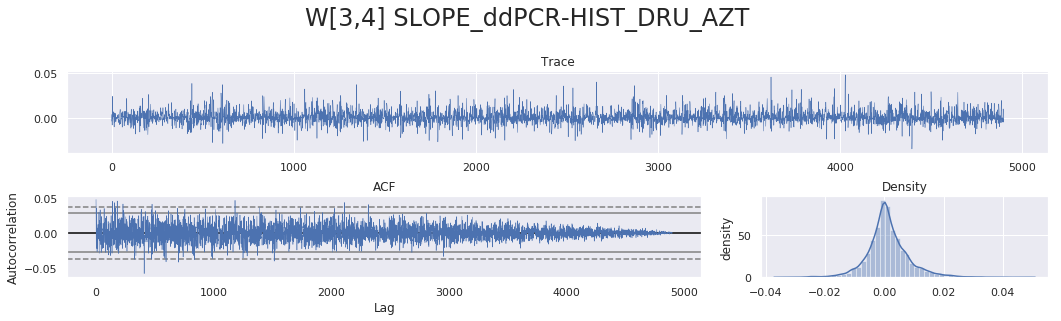
\includegraphics[width=0.9\linewidth]{HIV_MCMC_diag_l200}
		\caption{MCMC diagnostics for the Gibbs sampler with $\lambda=200$. Note that W in this case refers to $W_{12}$.}
		\label{fig:diagnostics200}
	}
	\qquad\qquad\qquad\\
	\qquad\qquad\qquad
	\subfloat{
		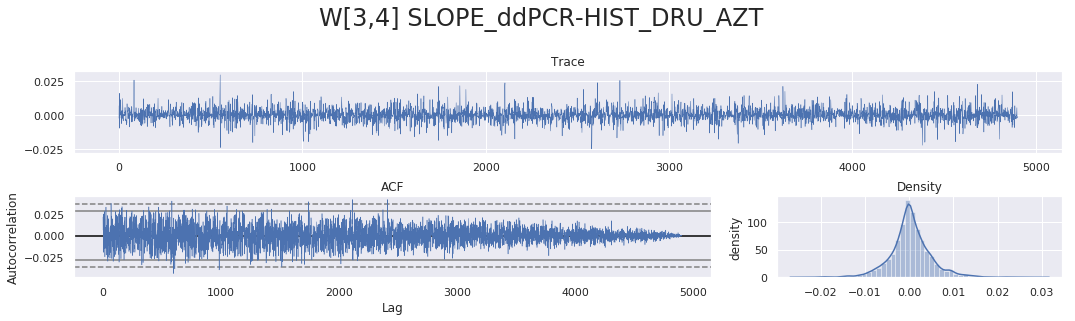
\includegraphics[width=0.9\linewidth]{HIV_MCMC_diag_l300}
		\caption{MCMC diagnostics for the Gibbs sampler with $\lambda=300$. Note that W in this case refers to $W_{12}$.}
		\label{fig:diagnostics300}
	}
	\qquad\qquad\qquad\\
	\qquad\qquad\qquad
	\subfloat{
		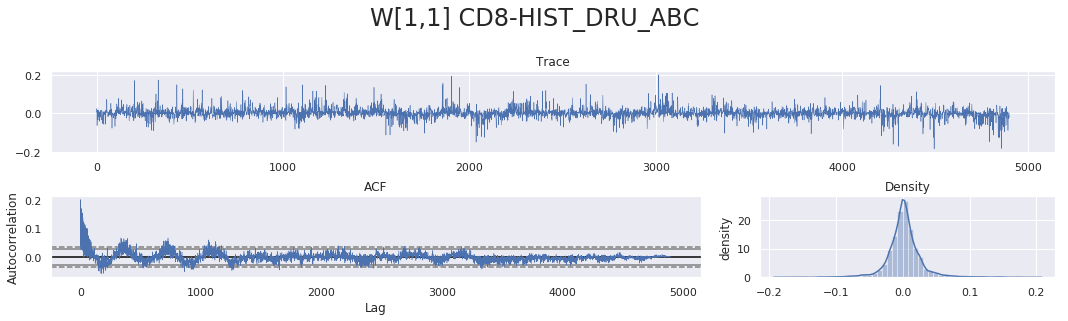
\includegraphics[width=0.9\linewidth]{HIV_MCMC_diag_l50}
		\caption{MCMC diagnostics for the Gibbs sampler with $\lambda=50$. Note that W in this case refers to $W_{12}$.}
		\label{fig:diagnostics50}
	}
\end{figure}




\subsection{Selection of Lambda and Threshold}
First of all, the network sizes for different $\lambda$ and thresholds were explored.
As we can see in \autoref{fig:heatmapSA}, Simulated Annealing leads to a smooth change in network size
over the range of $\lambda$ and thresholds explored, which is what we would expect.
This allows us to fix the thresholding while exploring the whole range of networks, from rather densely connected to completely sparse.
As we know that both precision and specificity tend to increase with network sparsity,
connections found in sparser networks (i.e. with higher $\lambda$) can be seen as more certain.
%%%%%%%%%%% HEATMAP SA
\begin{figure}[H]
	\centering
	\subfloat{
		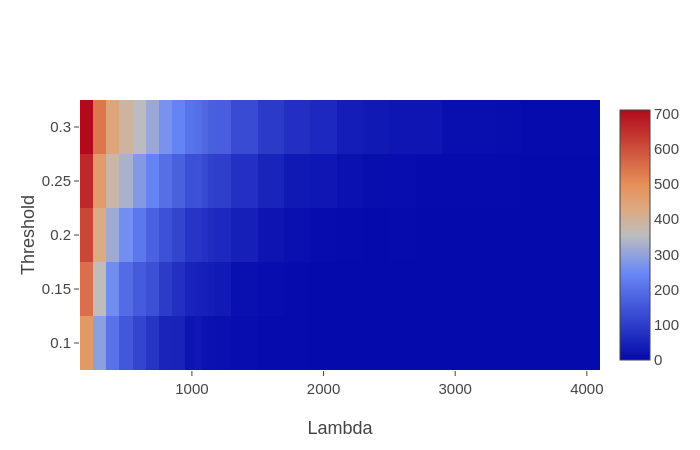
\includegraphics[width=0.48\linewidth]{HIV_SA_heat}
	}
	\subfloat{
		\includegraphics[width=0.48\linewidth]{HIV_SA_heat3d}
	}
	\caption{Heatmap and 3D surface plot showing the number of edges in the inferred networks with the SA BMB for different $\lambda$ and Credible Intervals (\gls{CI} defined by [threshold, 1-threshold]).}
	
	\label{fig:heatmapSA}
\end{figure}


In contrast, finding a suitable range of $\lambda$ for the Gibbs \gls{BMB} is quite difficult.
As shown in \autoref{fig:heatmapgibbs},  the resulting networks are non-trivial for reasonable Credible Intervals only in the multi-modal region $(\lambda<200)$.
But even then, the resulting networks are extremely sparse for 80\% Credible Intervals and above,
with a non-smooth and non-monotonic decrease in the number of edges for higher $\lambda$.
As with SA, we know the precision and specificity generally increases for higher $\lambda$ and sparser networks.
However, the usable range of $\lambda$ is very close to the range subject to convergence problems.
While we can clearly see that $\lambda$ of 50 and lower are unusable, it is not certain that slightly higher $\lambda$
are immune; it is possible, that similar problems are not obvious from mere inspection of the diagnostic plots.
Combined with non-monotonic change of network size, network and model exploration is made considerably more difficult.
%%%%%%%%%% HEATMAP gibbs
\begin{figure}[H]
	\centering
	\subfloat{
		\includegraphics[width=0.48\linewidth]{HIV_gibbs_heat}
	}
	\subfloat{
		\includegraphics[width=0.48\linewidth]{HIV_gibbs_heat3d}
	}
	\caption{Heatmap and 3D surface plot showing the number of edges in the inferred networks with the Gibbs BMB for different $\lambda$ and Credible Intervals (\gls{CI} defined by [threshold, 1-threshold]).}
	
	\label{fig:heatmapgibbs}
\end{figure}
\pagebreak

\subsection{Dependencies by Relevance}
Starting from the sparsest graph we can decrease the $\lambda$ in small steps and look at which edges are added.
It is important to note, that edges can in some cases vanish again for smaller $\lambda$.
That is, the network resulting from a higher $\lambda$ are not always subsets of the denser networks.
It is unclear, whether this is occurs due to convergence issues of the Annealing or simply is part of the models behavior.
Nonetheless, the increase in specificity and precision for higher $\lambda$ is still relevant.
\autoref{fig:HIVbylambda1} shows edges that have been observed for a $\lambda$ of 1400 and higher with a threshold of $0.15$.
The plotted bars correspond to the highest $\lambda$ they were observed at, i.e. the sparsest network that still contained them.

\begin{figure}
	\centering
	\includegraphics[width=1\linewidth]{HIV_bylambda}
	\caption{Maximum $\lambda$ for which each edge was observed with threshold $0.15$ and $\lambda>=1400$.}
	\label{fig:HIVbylambda1}
	
\end{figure}
We can see that about half of the dependencies there correspond to connections between the ddPCR counts (or its slope) and resistance relevant mutations from the haplotypes.
The two first edges correspond to the haplotype mutations PR69 and PR71.
According to \cite{shafer2017human}, PR69 is associated only with the \gls{PI} tipranavir,
which has shown to be effective for patients being resistant to other PIs \citep{doyon2005selection}.
Thus a mutation restricting the effectiveness of tipranavir being relevant for the HIV levels of treatment experienced patients seems reasonable.
PR71 is associated with multi-drug resistance for five different \gls{PI}s (of totally 8).
Considering that, this resistance can limit the range of possible \gls{PI} in a treatment considerably, making it an important factor for successful \gls{ART}.
In general we can see that a large portion of the first few dependencies correspond to resistances against protease inhibitors.
For the interested reader \autoref{fig:HIVbylambda2} additionally provides the edges found for $\lambda$ greater than 1000 and smaller than 1400.
We will not go into further details at this point and instead switch to the network graphs.
\begin{figure}[H]
	\centering
	\includegraphics[width=1\linewidth]{HIV_bylambda_1000p}
	\caption{Maximum $\lambda$ for which each edge was observed with threshold $0.15$ and $1000<\lambda<1400$.}
	\label{fig:HIVbylambda2}
	
\end{figure}
\subsection{Dependency Networks}
For comparing the networks resulting from the BMB and SA, we fix the graph size to 42 non-zero edges and then select a corresponding threshold and $\lambda$, which leads in our opinion to a network size that is still interpretable while not being trivial.
In case of the Annealing, we left the threshold fixed at $0.15$ with a $\lambda$ of 1100.
For the BMB, the threshold had to be finely tuned, resulting in a $\lambda$ of 70 with the threshold $0.22$.
In \autoref{fig:bignetworkcircle} and \autoref{fig:bignetworkcircle2} the network graphs are shown in a circular layout.
It can be seen, that the networks resulting from the BMB and the SA are rather similar.
Both exhibit a lot of connections with the lower section of the circle, which corresponds to the mutations calculated from the reconstructed haplotypes.
In contrast, there are barely any connections to the left side, i.e. the GRT mutations.
Simulated Annealing finds one dependency there, while the BMB does not show any.
The found edge corresponds to a positive partial correlation between MU\_PR77 affecting 3 different \gls{PI}s and the ddPCR slope, indicating a deterioration caused by the mutation.
However, it is unclear why barely any interactions with the GRT mutations are present in the networks.
Examining GRT mutations for planning the next step in a antiretroviral therapy is currently a standard practice, due to the shown improvements in terms of therapy success \cite{gunthard2018human}.
Instead of assuming a lack of dependency between the clinical factors and the GRT mutations, this might indicate that the mutations inferred from the haplotypes are more accurate,
thus making the GRT mutations mostly redundant when conditioning on the haplotypes.

%%%%%%%% BIG NETWORK CIRCLE
\begin{figure}
	\centering
	\includegraphics[width=0.72\linewidth]{HIV_gibbs_bigcircle}
	
	\caption{W12 subnetwork estimated with Gibbs BMB.}
	\label{fig:bignetworkcircle}
\end{figure}
\begin{figure}
	\centering
	\subfloat{
		\includegraphics[width=0.72\linewidth]{HIV_SA_bigcircle}
		\caption{W12 subnetwork estimated with SA.}
		\label{fig:bignetworkcircle2}
	}
	
\end{figure}
\autoref{fig:network_gibbs} and \autoref{fig:network_SA} show the the same networks with a different layout.
Here we can see that a lot of haplotype mutations form a cluster around the ddPCR values (in case of the SA also around the slope).
While the connections themselves seem reasonable, the signs of the partial correlations are counter-intuitive.
A red edge corresponds to a negative partial correlation.
Consequently, a lot of haplotype mutations would seem to result in a decrease of the HIV levels.
Instead, we would have expected an increase, as the resistance relevant mutations generally inhibit the effectiveness of specific drugs.
Furthermore, we can see that ETC and TDF have a positive edge to the CD4 values, while simultaneously being negatively correlated with the CD8 counts. 
In the initial phase of HIV infection, the CD8 counts increase significantly and are followed by a decrease of CD4 counts.
In addition the ratio of CD4 to CD8 counts is known to be a marker for the clinical outcome in virologically suppressed HIV patients \citep{lu2015cd4} and elevated CD8 counts during ART are associated with failure in antiretroviral therapy \citep{krantz2011elevated}.
As a consequence, we can assume that the positive correlation with CD4 and negative correlation with CD8 counts corresponds to the ETC and TDF having a positive impact on treatment success.

An interesting connection that is present in both networks (see \autoref{fig:intersection}) is the positive partial correlation between RNA and the drug \gls{D4T},
with the Gibbs BMB also showing an edge to HIST\_D4T.
\gls{D4T} is a \gls{NRTI}, meaning that it blocks the enzyme responsible for changing RNA into the form of DNA.
While being largely used in the past as a initial treatment for patients with advanced immunodeficiency \footnote{\href{http://www.aidsmap.com/d4T-stavudine-iZeriti/page/1730937/}{http://www.aidsmap.com/d4T-stavudine-iZeriti/page/1730937/}}
the \gls{WHO} no longer recommends its use due to side effects
 \footnote{
 	\href{http://www.who.int/hiv/pub/guidelines/arv2013/arv2013supplement_to_chapter09.pdf}
	{http://www.who.int/hiv/pub/guidelines/arv2013/arv2013supplement\_to\_chapter09.pdf}}.
The connection might indicate that patients starting treatment at a later stage show a higher tendency for exhibiting blips in therapy.
In any case, the connections between viral load and \gls{ART} drugs do not shed any light on the controversial effects of the blips on developing new resistance mutations.


%% -> Networks: BMB + SA
\begin{figure}
	\centering
	\makebox[\textwidth][c]{
		\includegraphics[width=1.2\linewidth]{HIV_gibbs_network}
	}
	\caption{Inferred network with Gibbs BMB, using $\lambda$ = 70 and threshold $0.22$.}
	\label{fig:network_gibbs}
\end{figure}
\begin{figure}
	\centering
	\makebox[\textwidth][c]{
		\includegraphics[width=1.2\linewidth]{HIV_SA_network}
	}
	
	\caption{Inferred network with Simulated Annealing, using $\lambda$ = 1100 and threshold $0.15$.}
	
	\label{fig:network_SA}
\end{figure}
\begin{figure}
	\centering
	\includegraphics[width=0.9\linewidth]{HIV_intersection_network}
	\caption{Intersection of the SA and BMB network. Black edges indicate a disagreement in the sign of the edge.}
	
	\label{fig:intersection}
\end{figure}

\FloatBarrier
\subsection{Latent Scores}
\autoref{fig:zscores} and \autoref{fig:zscores_bool} illustrate the effect of the copula transformation on the data
for 2100 Gibbs sweeps with a burn-in of 630 and a $\lambda$ of 1000.
The first column shows the distribution of untransformed observations for one variable;
the second, the distribution of the normal scores (which are used for initialization);
the third column shows the distribution of the posterior mean of the latent values.
That is, the histogram of the estimated $E[z_{i,j}|\matr{Z}\in D, \lambda=1000]$ for all observations $i$ with fixed variable $j$.
The distributions did not show any significant change with further iteration of the sampler.
The latent values of the remaining query variables are not displayed for the sake of compactness, since they did not show 
any unusual behavior.

\begin{figure}[H]
	\centering
	
	\subfloat{
		\includegraphics[width=0.9\linewidth]{HIV_Zscores_RNA}
	}
	\subfloat{
		\includegraphics[width=0.9\linewidth]{HIV_Zscores_ddpcr}
	}
	\caption{Initial distribution of the data compared to the distribution of the estimated latent values.}
	\label{fig:zscores}
\end{figure}
The semi-parametric copula seems to be troubled mainly when the data is highly imbalanced with a lot of identical values.
While the estimated latent values for the ddPCR count and even the boolean HIST\_DRU\_3TC are relatively normal,
the viral load (RNA) and the GRT mutations (in this case MU\_RT70) seem to be flawed.
The RNA is similar to the GRT mutations in the sense that it has the majority of samples at the same value $0$,
with the exception of a few blips.
In contrast, the variables indicating the per-drug treatment-experience are more balanced.
Additionally, the mutations inferred from the haplotypes contain a lot of missing values, which are filled by the copula sampler
with normal draws.
That the unbalanced GRT mutations do seemingly not converge to a normal distribution might be related to the failure to find dependencies shared with the query variables.

\begin{figure}
	\subfloat{
		\includegraphics[width=0.9\linewidth]{HIV_Zscores_HIST3tc}
	}
	\subfloat{
		\includegraphics[width=0.9\linewidth]{HIV_Zscores_PR13}
	}
	\subfloat{
		\includegraphics[width=0.9\linewidth]{HIV_Zscores_MU_RT70}
	}
	\caption{Initial distribution of the data compared to Z estimated by averaging over the draws. The second column corresponds to the distribution of the normal scores, the last column to the mean over all draws.}
	\label{fig:zscores_bool}
\end{figure}
%% -> Latent Variables: Not fully normal
%% -> Talk about connections found
\chapter{Conclusion and Future Work}
In this work we have introduced Simulated Annealing as an alternative estimation procedure for the Markov Blanket.
While the Annealing MAP did not result in performance competitive to the GLASSO, it was shown to be comparable to the previous approach by \cite{kaufmann_bayesian_2015}.
In addition, SA has proven to be more robust in its application on the HIV-X data set by allowing for a smoother process of network selection, while the BMB gave unexpected problems.
The feasible $\lambda$ region of the BMB lies closely to the region subject to convergence problems of the Markov chains, thus making the inferred networks less certain.
In the test data however, SA had the disadvantage of an upper limit on the sparsity, presumably due to numerical instability.
We assume that this instability mainly stems from the MGIG distributed $\Wxx$ posterior conditional. 

In applications of both models, we could identify multi-modality of the posterior marginal of $\Wxy$ for small $\lambda$, while posterior marginals for higher $\lambda$ seem to be unimodal.
This is also reflected in the Annealing behavior, as the sampler starts fluctuating between multiple modes when in the corresponding $\lambda$ region.

Finally, the application on the HIV-X dataset indicated that the GRT mutations may not have a significant effect on the clinical factors in comparison to the haplotype mutations. However, it is unclear whether the seemingly non-normal distributions of the latent values for the GRT mutations influenced this result.
 Although we could identify some connections in the networks that are agreeable with known results, a lot of edges express counter-intuitive partial correlations.
For example, multiple resistance relevant mutations are negatively correlated with the ddPCR HIV cell count.


\section*{Future Work}
One of the main shortcomings of the model underlying the BMB is the reliance on the MGIG distribution.
In general, the MGIG proves to be difficult both in theory and practice due to the suboptimal methods available for sampling from it.
Thus future work could be focused on finding an different sampling method.
A possible alternative for directly sampling the MGIG would be substituting the draw of the MGIG with a draw from the $\Wxx$ marginal $P(\Wxx|\matr{T}, \matr{S}, \lambda)$.
While the marginal does not offer a closed form solution in terms of a known distribution, we can use a Metropolis Hastings sampler.
Due to the similarity, we would suggest the Wishart arising from the special case of $P(\Wxx|\matr{T}, \matr{S}, \lambda)$ for $\matr{D}\rightarrow\matr{0}$ (see \autoref{ss:postmarginal}) as proposal function.
The difference between the special case and the general case of the marginal posterior lies in the determinant:
$$\det
\Big(
(\matr{S}_{22} + \matr{I}) \otimes \matr{W}_{11}^{-1} +\matr{D}
\Big)$$
We know that $A=((\matr{S}_{22} + \matr{I}) \otimes \matr{W}_{11}^{-1})$ is symmetric and positive definite (so all eigenvalues of $A$ are positive), and $\matr{D}$ is a diagonal matrix with positive entries.
With $\det(A)=\prod_{i}\lambda_i$ and $tr(A) = \sum_i \lambda_i$ it's clear to see
that
$$\det\Big((\matr{S}_{22} + \matr{I}) \otimes \matr{W}_{11}^{-1} + \matr{D}\Big) > \det\Big((\matr{S}_{22} + \matr{I}) \otimes \matr{W}_{11}^{-1}\Big)
$$
As only the normalization differs, we assume that the general case of the posterior marginal is a flatter version of the special case.
Additionally, $\matr{D}$ tends to be quite small in practice, so the special case should serve as a good proposal function with a high acceptance rate.
\\\\
Another interesting point would be adjusting the synthetic data to a more general setting.
We have seen that the usability of the Annealing approach played a big role for the application on real data.
However, the cause of this difference compared to the BMB is unclear, as the tests on artificial data did not indicate similar problems.
While the artificial data does reflect the small world property of real problems, the already normally distributed data presumably obsoletes the semi-parametric copula.
In contrast, many realistic use cases with mixed data rely on the copula transformation,
which should motivate the use of a more appropriate data set.
Because of this, we would suggest comparing the BMB and the Annealing on unbalanced and sparse data (similar to the mutations) that still exhibits small world properties.

%\input{./Chapters/Chapter7}
%% ----------------------------------------------------------------
\thesisappendix
\thesisbib
\begin{appendices}
	\chapter{Appendix}
\section{Distributions}
\subsection{Matrix Generalized Inverse Gaussian}
The Matrix \gls{MGIG} distribution is a probability distribution over positive definite symmetric ($pxp$) matrices $\{X:X>0\}$ \citet{butler_generalized_1998}.
It has recently been shown to be unimodal \citep{fazayeli2016matrix}.

\subsubsection{Butler Parameterization}
\label{MGIG_BUTLER}
In the models we mostly denote the \gls{MGIG} by the parametrization of \citet{butler_generalized_1998}
as it is the most commonly used one.
\begin{equation}
\matr{X} \sim \mathcal{MGIG}_{B}(\lambda, \matr{A}, \matr{B}) 
\end{equation}
\begin{equation*}
p(\matr{X}) \propto \det(\matr{X})^{\lambda - \frac{1}{2}(p+1)}
\exp \tr
\Big(
	-\frac{1}{2} (\matr{A}\matr{X} + \matr{B} \matr{X}^{-1} )
\Big)
\end{equation*}

\subsubsection{Letac Parameterization}
\label{MGIG_LETAC}
For sampling from the \gls{MGIG}, we use a notation similar to the one used for the \gls{GIG} in \cite{letac1983characterization}.
\begin{equation}
\matr{X} \sim \mathcal{MGIG}_{L}(n', \matr{A}, \matr{B}) 
\end{equation}
\begin{equation*}
p(\matr{X}) \propto \det(\matr{X})^{-n' - 1}
\exp \tr
\Big(
-\frac{1}{2} (\matr{A}\matr{X} + \matr{B} \matr{X}^{-1} )
\Big)
\qquad
n'>\frac{p-1}{2}
\end{equation*}

\section{Model}
\label{A:model}
\begin{math}
\\
\begin{array}{lclr}
\matr{x}_{1,\dots,n} &\overset{iid}{\sim}& \mathcal{N}_{(p+q)}(0, \matr{\Sigma})
\\
\matr{X}&=&(\bm{x}_1,\dots,\bm{x}_n)  & \matr{X}\in \mathbb{R}^{(p+q)\times n}
%\quad
\\ \\
\matr{S} &=& \matr{X} \matr{X}^T
\\
\matr{S} &\sim& \mathcal{W}_{p+q}(n, \matr{\Sigma})
\end{array}
\end{math}
\\
\\
\begin{equation*}
\matr{\Sigma^{-1}} = \matr{W}=
\raisebox{0.3\baselineskip}{$
	\begin{blockarray}{ccc}
	p & q& \\
	\begin{block}{(cc)l}
		\matr{W}_{11} & \matr{W}_{12}&p \\
		\matr{W}_{12}^T & \matr{W}_{22}&q \\
	\end{block}
	\end{blockarray}
$}
\quad \quad \quad \quad 
\matr{S}=
\raisebox{0.3\baselineskip}{$
	\begin{blockarray}{ccc}
	p & q& \\
	\begin{block}{(cc)l}
	\matr{S}_{11} & \matr{S}_{12}&p \\
	\matr{S}_{12}^T & \matr{S}_{22}&q \\
	\end{block}
	\end{blockarray}
	$}
\end{equation*}
\\ \\
Let 
$$\matr{W}_{22.1} = \matr{W}_{22} - \matr{W}_{12}^T \matr{W}_{11}^{-1} \matr{W}_{12}$$
be the Schur complement of $\matr{W}_{22}$.


\subsection{Likelihood}

\begin{align*}
p(\matr{S}|\matr{W}) &\propto \det(\matr{W})^{\frac{n}{2}} det(\matr{S})^{\frac{n-(p+q)-1}{2} }\exp \tr \big( - \frac{1}{2} \matr{W} \matr{S}\big)
\end{align*}

\subsection{Prior}
\begin{align*}
P(\matr{W}|\matr{T}) &=
\mathcal{W}_{p+q} \big(p + q + 1, \matr{I}\big) p(\matr{W}_{12} | \matr{T} )
\\
&\propto \exp\tr \Big(-\frac{1}{2} \matr{W}\Big)
\prod_{{\substack{i=1,\dots,p\\j=1,\dots,q}} }   \frac{1}{\sqrt{2\pi \matr{T}_{ij}}} \exp 
\Big( - \frac{(\matr{W}_{12})_{ij}^2}{2\matr{T}_{ij}} \Big) 
\\ \\
P(\matr{T}| \lambda) &\propto
\prod_{{\substack{i=1,\dots,p\\j=1,\dots,q}} }   \frac{\lambda^2}{2} \exp \Big( - \frac{\lambda^2}{2} \matr{T}_{ij} \Big)
\end{align*}
\subsection{Joint Distribution}
\begin{align*}
p(\matr{W}, \matr{S}, \matr{T} | \lambda) =& p(\matr{W}_{11}, \matr{W}_{12}, \matr{W}_{22}, \matr{S}, \matr{T} | \lambda) \\
\propto& \quad \det(\matr{W})^\frac{n}{2} 
\det(\matr{S})^{\frac{n-(p+q)-1}{2} }
\\
&\times \exp \tr \big( - \frac{1}{2} \matr{W} \matr{S}\big)		
 \exp\tr \Big(-\frac{1}{2} \matr{W}\Big)
\\
&\times \prod_{{\substack{i=1,\dots,p\\j=1,\dots,q}} }  \frac{1}{\sqrt{2\pi \matr{T}_{ij}}} \exp 
\Big( - \frac{(\matr{W}_{12})_{ij}^2}{2\matr{T}_{ij}} \Big) 
\\
&\times \prod_{{\substack{i=1,\dots,p\\j=1,\dots,q}} } \frac{\lambda^2}{2} \exp \Big( - \frac{\lambda^2}{2} \matr{T}_{ij} \Big)
\\\\
= &\det(\matr{W})^{\frac{n}{2}}  \det(\matr{S})^{\frac{n-(p+q)-1}{2}} 
\\
&\exp\Bigg(-\frac{1}{2} \tr [\matr{WS}+\matr{W}] - \frac{1}{2} \sum_{{\substack{i=1,\dots,p\\j=1,\dots,q}} } \frac{(\matr{W}_{12})_{ij}^2}{\matr{T}_{ij}}  \Bigg) 
\\
&\times \Big[\prod_{{\substack{i=1,\dots,p\\j=1,\dots,q}} }  \frac{1}{\sqrt{2\pi \matr{T}_{ij}}}\Big]
p(\matr{T}|\lambda)
\end{align*}
\subsubsection{Reparametrization with $\matr{W}_{11}, \matr{W}_{12}, \matr{W}_{22.1}$}
$$ J\big((\matr{W}_{11}, \matr{W}_{12}, \matr{W}_{22}) \rightarrow (\matr{W}_{11}, \matr{W}_{12}, \matr{W}_{22.1})\big) = \matr{1} $$
\begin{align*}
\det(\matr{W}) &= \det(\matr{W}_{11}) \det(\matr{W}_{22} - \matr{W}_{12}^T \matr{W}_{11}^{-1}\matr{W}_{12})
\\
&= \det(\matr{W}_{11}) \det(\matr{W}_{22.1})
\\
\\
\tr(\matr{WS}) &= \tr\big[\matr{W}_{11}\matr{S}_{11} + \matr{W}_{12}\matr{S}_{21} + \matr{W}_{21}\matr{S}_{12} + \matr{W}_{22}\matr{S}_{22}   \big]
\\
&= \tr\big[\matr{W}_{11}\matr{S}_{11} + \matr{W}_{12}\matr{S}_{12}^T + \matr{W}_{12}^T\matr{S}_{12} + (\matr{W}_{22.1} + \matr{W}_{12}^T\matr{W}_{11}^{-1}\matr{W}_{12}) \matr{S}_{22}   \big]
\\
&= \tr\big[
\Cline[blue]{\matr{W}_{11}\matr{S}_{11}} + 
\Cline[yellow]{\matr{W}_{12}\matr{S}_{12}^T + 
	\matr{W}_{12}^T\matr{S}_{12}} + 
\Cline[red]{\matr{W}_{22.1}\matr{S}_{22}} + 
\Cline[green]{\matr{W}_{12}^T\matr{W}_{11}^{-1}\matr{W}_{12}\matr{S}_{22}}   
\big]
\\
\\
\tr(\matr{W}) &= \tr(\matr{W}_{11}) + \tr(\matr{W}_{22})
\\
&= \tr(\Cline[blue]{\matr{W}_{11}}) + 
\tr(\Cline[red]{\matr{W}_{22.1}}) +
\tr(\Cline[green]{\matr{W}_{12}^T\matr{W}_{11}^{-1}\matr{W}_{12}})
\end{align*}

\begin{align*}
p(\matr{W}_{11}, \matr{W}_{12}, &\matr{W}_{22.1}, \matr{S}, \matr{T} | \lambda) \propto
\\
&\det(\matr{W}_{11})^{n/2} \det(\matr{W}_{22.1})^{n/2} \det(\matr{\matr{S}})^{\frac{n-(p+q)-1}{2}}
\\
\times& \exp \Big(
-\frac{1}{2}
\tr\big[
\Cline[blue]{\matr{W}_{11} (\matr{S}_{11} + \matr{I}) }+ 
\Cline[red]{\matr{W}_{22.1}  (\matr{S}_{22} + \matr{I})} + 
\\
&\quad \quad \quad \quad \quad \quad
\Cline[yellow]{2 (\matr{W}_{12}^T\matr{S}_{12})} +
\Cline[green]{
	\matr{W}_{12}^T \matr{W}_{11}^{-1}\matr{W}_{12} 
	(\matr{S}_{22} + \matr{I})}
\big]
\Big)
\\
\times& \exp\Big(- \frac{1}{2} \sum_{{\substack{i=1,\dots,p\\j=1,\dots,q}} } \frac{(\matr{W}_{12})_{ij}^2}{\matr{T}_{ij}} \Big) \quad \Big[\prod_{{\substack{i=1,\dots,p\\j=1,\dots,q}} }  \frac{1}{\sqrt{2\pi \matr{T}_{ij}}}\Big]
\quad
p(\matr{T}|\lambda)
\end{align*}

\subsection{Full Posterior}
Let $\matr{D} = \text{diag}(\text{vec}(\matr{T}))^{-1}$, i.e. a diagonal matrix, where the elements are the inverses of the elements of $\matr{T}$

\begin{align*}
\exp\Big(- \frac{1}{2}  \sum_{{\substack{i=1,\dots,p\\j=1,\dots,q}} } \frac{(\matr{W}_{12})_{ij}^2}{\matr{T}_{ij}} \Big)
&= 
\exp \Big(
-\frac{1}{2} \Cline[gray]{\text{vec}(\matr{W}_{12})^T\  \matr{D} \ \text{vec}(\matr{W}_{12})
}
\Big)
\\
\\
\tr(\Cline[yellow]{\matr{W}_{12}^T \matr{S}_{12}})  &= \text{vec}(\matr{W}_{12})^T \text{vec}(\matr{S}_{12})
\end{align*}


\begin{align}
p(\matr{W}_{11}, \matr{W}_{12}, \matr{W}_{22.1}, \matr{T} | \matr{S}, \lambda) \propto 
&\det(\matr{W}_{11})^{n/2} \exp \Big( - \frac{1}{2} \tr\big[ \Cline[blue]{\matr{W}_{11} (\matr{S}_{11} + \matr{I}) }\big]\Big)
\label{joint_1}\\
&\times \det(\matr{W}_{22.1})^{n/2} \exp \Big( - \frac{1}{2} \tr\big[ \Cline[red]{\matr{W}_{22.1}  (\matr{S}_{22} + \matr{I})}\big]\Big)
\nonumber\\
&\times \exp\Big(
-\frac{1}{2} \tr \big[ \Cline[green]{\matr{W}_{12}^T\matr{W}_{11}^{-1}\matr{W}_{12}\big(\matr{S}_{22}+\matr{I}\big)}   \big]
\Big)
\nonumber\\
&\times \exp \Big(
-\frac{1}{2} 
\Cline[gray]{
	\text{vec}(\matr{W}_{12})^T\  \matr{D} \ \text{vec}(\matr{W}_{12})
}
\Big)
\nonumber\\
&\times \exp \Big( 
\Cline[yellow]{
	-\text{vec}(\matr{W}_{12})^T \text{vec}(\matr{S}_{12})\Big)
}
\nonumber\\
&\times \Big[\prod_{{\substack{i=1,\dots,p\\j=1,\dots,q}} }  \frac{1}{\sqrt{2\pi \matr{T}_{ij}}}\Big]
p(\matr{T} | \lambda)
\nonumber\\\nonumber \\
\nonumber\\
\tr \Big[ \Cline[green]{\matr{W}_{12}^T \matr{W}_{11}^{-1}\matr{W}_{12}(\matr{S}_{22}+\matr{I})}\Big]
&= \text{vec}(\matr{W}_{12})^T \text{vec}(\matr{W}_{11}^{-1} \matr{W}_{12}(\matr{S}_{22} + \matr{I} ))
\nonumber\\
&\overset{\text{\tiny{(520 Matr. Cookbook)}}}{=}
\text{vec}(\matr{W}_{12})^T \Big[
(\matr{S}_{22} + \matr{I})^T \otimes \matr{W}_{11}^{-1} \Big]
\text{vec}(\matr{W}_{12})
\nonumber\\
&= \text{vec}(\matr{W}_{12})^T \Big[
(\matr{S}_{22} + \matr{I}) \otimes \matr{W}_{11}^{-1} \Big]
\text{vec}(\matr{W}_{12})
\nonumber\\
\nonumber\\  \nonumber\\
p(\matr{W}_{11}, \matr{W}_{12}, \matr{W}_{22.1}, \matr{T} | \matr{S}, \lambda) \propto&
\det(\matr{W}_{11})^{n/2} \exp \Big( - \frac{1}{2} \tr\big[ \matr{W}_{11} (\matr{S}_{11} + \matr{I}) \big]\Big)
\label{joint_2}\\
&\times \det(\matr{W}_{22.1})^{n/2} \exp \Big( - \frac{1}{2} \tr\big[\matr{W}_{22.1}  (\matr{S}_{22} + \matr{I})\big]\Big)
\nonumber\\
&\times \exp\Big(
-\frac{1}{2}\Cline[gray]{\Cline[green]{\text{vec}(\matr{W}_{12})^T \Big[
		(\matr{S}_{22} + \matr{I}) \otimes \matr{W}_{11}^{-1} +\matr{D}\Big]
		\text{vec}(\matr{W}_{12})}}
- \text{vec}(\matr{W}_{12})^T \text{vec}(\matr{S}_{12})
\Big)
\nonumber\\
&\times \Big[\prod_{{\substack{i=1,\dots,p\\j=1,\dots,q}} }  \frac{1}{\sqrt{2\pi \matr{T}_{ij}}}\Big]
p(\matr{T}|\lambda)
\nonumber
\end{align}
\subsubsection{Factorization of the Posterior}
\label{A:factorized_post}
We can now factorize wrt. $W_{22.1}$.
$$ p(\matr{W}_{11}, \matr{W}_{12}, \matr{W}_{22.1}, \matr{T} | \matr{S}, \lambda)
= p(\matr{W}_{11}, \matr{W}_{12}, \matr{T} | \matr{S}, \lambda) p(\matr{W}_{22.1} | \matr{S}, \lambda) 
$$

Using
\begin{align*}
\det(\matr{S})^{\frac{n-(p+q)-1}{2}} &= \det(\Syy)^{\frac{n-p-q-1}{2}} \det(\Sxxs)^{\frac{n-p-q-1}{2}}
\\
&=
\det(\Syy)^{\frac{n-p-2q-1}{2}}\det(\Syy^{-1})^{-\frac{q}{2}} \det(\Sxxs)^{\frac{n-p-q-1}{2}}
\end{align*}
It follows that

\begin{align}
\label{A:W221}
p(\Wyys|\matr{S}, \lambda)
\propto 
\det(\Syy)^{\frac{n-p-q-1}{2}}
\det(\Wyys)^{\frac{n}{2}}
\exp\big(
	-\frac{1}{2} \tr \big[
		\Wyys (\Syy+\matr{I})
	\big]
\big)
\end{align}
Comparing the determinants of \autoref{A:W221} to the ones from the Wishart (denoted by $df$, furthermore we know the size of the Wishart distributed matrix is $q$):
\begin{align*}
\det(\Wyys)^{\frac{df-q-1}{2}} &= \det(\Wyys)^{\frac{n}{2}}
\\
\det(\Syy)^{\frac{df}{2}} &= \det(\Syy)^{\frac{n-p-2q-1}{2}}
\end{align*}
\begin{align*}
\Rightarrow&
q = df - n - 1
\\
&df = n -p-2q-1
\\
&\quad= n-p-2(df-n-1)-1
\\
\Rightarrow&
3df = 3n - p + 1
\\
\Rightarrow&
df = n- \frac{(p-1)}{3}
\end{align*}
$$\Downarrow$$
\begin{equation}
\boxed{
	\Wyys|\matr{S}, \lambda \sim \mathcal{W}\Big(n-\frac{(p-1)}{3}, \Syy \Big)
	}
\end{equation}
\\
\\

Additionally, now the joint posterior for $(\Wxx, \Wxy)$ is:
\begin{align}
p(\matr{W}_{11}, \matr{W}_{12}, \matr{T} | \matr{S}, \lambda)
\propto& \quad
\det(\matr{W}_{11})^{n/2} \exp \Big( - \frac{1}{2} \tr\big[ \matr{W}_{11} (\matr{S}_{11} + \matr{I}) \big]\Big)
\label{marginal_joint}\\
&\times \exp\Big(
-\frac{1}{2}\text{vec}(\matr{W}_{12})^T \Big[
(\matr{S}_{22} + \matr{I}) \otimes \matr{W}_{11}^{-1} +\matr{D}\Big]
\text{vec}(\matr{W}_{12})
- \text{vec}(\matr{W}_{12})^T \text{vec}(\matr{S}_{12})
\Big)
\nonumber \\
&\times \Big[\prod_{{\substack{i=1,\dots,p\\j=1,\dots,q}} }  \frac{1}{\sqrt{2\pi \matr{T}_{ij}}}\Big]
p(\matr{T}|\lambda)
\nonumber
\end{align}
\subsection{Posterior Conditionals}
\label{A:post_cond}
\subsubsection{$\matr{W}_{12}$}
We condition \autoref{marginal_joint} additionally on $\matr{T}$ and $\matr{W}_{11}$:

\begin{align*}
p(\matr{W}_{12} | \matr{W}_{11}, \matr{T}, \matr{S}, \lambda)
&\propto 
\exp\Big(
-\frac{1}{2}\text{vec}(\matr{W}_{12})^T \Big[
(\matr{S}_{22} + \matr{I}) \otimes \matr{W}_{11}^{-1} +\matr{D}\Big]
\text{vec}(\matr{W}_{12})
- \text{vec}(\matr{W}_{12})^T \text{vec}(\matr{S}_{12})
\Big)
\\
&=\exp\Big(-\frac{1}{2} x^T\matr{C}x - b^Tx\Big) 
\\
&\overset{\text{\tiny{(8.16Matr. Cookbook)}}}{=}
\exp \Big(-\frac{1}{2} (x+\matr{C}^{-1}b)^T\matr{C}(x+\matr{C}^{-1}b) + \frac{1}{2}b^T\matr{C}^{-1}b\Big)
\end{align*}

with 
$$
x = \text{vec}(\matr{W}_{12})
\quad \quad \quad
\matr{C} = \Big[
(\matr{S}_{22} + \matr{I}) \otimes \matr{W}_{11}^{-1} +\matr{D}\Big]
\quad \quad \quad
b = \text{vec}(\matr{S}_{12})
$$
$$\Downarrow$$
\begin{equation}
	\boxed{
		\text{vec}(\matr{W}_{12}) | \matr{W}_{11}, \matr{T}, \matr{S}, \lambda \sim \mathcal{N}(-\matr{C}^{-1} \text{vec}(\matr{S}_{12}), \matr{C}^{-1})
	}
\end{equation}

\subsubsection{$\matr{W}_{11}$}
We take \autoref{joint_1}, marginalize wrt. $\matr{W}_{22.1}$ and then additionally condition on $ \matr{W}_{12}, \matr{T}$:

\begin{align*}
p(\matr{W}_{11} | \matr{W}_{12}, \matr{T}, \matr{S}, \lambda)
& \propto
\det(\matr{W}_{11})^{n/2}
\exp \Big(
-\frac{1}{2} \tr\big[
\matr{W}_{11}(\matr{S}_{11}+ \matr{I}) + \matr{W}_{12}(\matr{S}_{22}+\matr{I})\matr{W}_{12}^T \matr{W}_{11}^{-1}
\big]
\Big)
\\
&=
\det(\matr{W}_{11})^{n/2}
\exp \Big(
-\frac{1}{2} \tr\big[
\underbrace{(\matr{S}_{11}+ \matr{I})}_{\text{MGIG A}} \matr{W}_{11}+ \underbrace{\matr{W}_{12}(\matr{S}_{22}+\matr{I})\matr{W}_{12}^T}_{\text{MGIG B}}\matr{W}_{11}^{-1}
\big]
\Big)
\end{align*}
$$\Downarrow$$
Comparing the determinants to the (Butler) \gls{MGIG} defined in \autoref{MGIG_BUTLER} leads to
\begin{equation}
\label{W11_MGIG_posterior}
\boxed{
	\matr{W}_{11} | \matr{W}_{12}, \matr{T}, \matr{S}, \lambda \sim 
	\mathcal{MGIG}_B
	\Big(
		\frac{n+p+1}{2}, \ 
		\matr{S}_{11}+\matr{I},\  
		\matr{W}_{12}(\matr{S}_{22}+\matr{I})\matr{W}_{12}^T
	\Big)
}
\end{equation}

\subsubsection{$\matr{T}$}
\begin{align*}
p(\matr{T}| \matr{W}_{11}, \matr{W}_{12}, \matr{S}, \lambda) \propto& 
\prod_{{\substack{i=1,\dots,p\\j=1,\dots,q}} }   \frac{1}{\sqrt{2\pi \matr{T}_{ij}}} \exp 
\Big( - \frac{(\matr{W}_{12})_{ij}^2}{2\matr{T}_{ij}} \Big) 
\prod_{{\substack{i=1,\dots,p\\j=1,\dots,q}} }   
\frac{\lambda^2}{2} 
\exp\Big( 
- \frac{\lambda^2}{2} \matr{T}_{ij} 
\Big)
\\
\\
p(\matr{T}_{ij}| \matr{W}_{11}, \matr{W}_{12}, \matr{S}, \lambda) \propto& 
\frac{1}{\sqrt{2\pi \matr{T}_{ij}}} \exp 
\Big( - \frac{(\matr{W}_{12})_{ij}^2}{2\matr{T}_{ij}} \Big)    
\frac{\lambda^2}{2} 
\exp\Big( 
- \frac{\lambda^2}{2} \matr{T}_{ij} 
\Big)
\\
=& \frac{\lambda^2}{2} \Big(\frac{1}{2\pi \matr{T}_{ij}}\Big)^{1/2} \exp \Big(-\frac{(\matr{W}_{12})_{ij}^2}{2\matr{T}_{ij}} - \frac{\lambda^2}{2} \matr{T}_{ij}\Big)
\end{align*}
Substitute $\matr{T}_{ij}$ with $\matr{T}_{ij}^{-1}$:
$
\quad
J(\matr{T}_{ij} \rightarrow \matr{T}_{ij}^{-1}) = -\matr{T}_{ij}^{-2}
$

\begin{align*}
p\Big(\frac{1}{\matr{T}_{ij}}\Big) \propto&
 -\matr{T}_{ij}^{-2} \frac{\lambda^2}{2}
\Big(
	\frac{1}{2\pi\matr{T}_{ij}^{-1}}
\Big)^{1/2} 
\exp \Big(
	- \frac{(\matr{W}_{12})_{ij}^2}{2}\matr{T}_{ij} - \frac{\lambda^2}{2}\matr{T}_{ij}^{-1}
\Big)
\\
=&
- \frac{\lambda^2}{2}
\Big(
	\frac{1}{2\pi\matr{T}_{ij}^{3}}
\Big)^{1/2} 
\exp \Big(
	- \frac{(\matr{W}_{12})_{ij}^2}{2\matr{T}_{ij}}
	\Big(
	\matr{T}_{ij}^2 - \frac{\lambda^2}{(\matr{W}_{12})_{ij}^{2}}
	\Big)
\Big)
\\
\\
&\text{Substitute }(\mu')^2 = \frac{\lambda^2}{(\matr{W}_{12})_{ij}^2}
\\
\\
=& 
- \frac{\lambda^2}{2}
\Big(
\frac{1}{2\pi\matr{T}_{ij}^{3}}
\Big)^{1/2} 
\exp \Big(
- \frac{\lambda^2}{2(\mu')^2\matr{T}_{ij}} \big(\matr{T}_{ij}^2 - 2 \matr{T}_{ij} \mu' + 2\matr{T}_{ij}\mu' + (\mu')^2 \big)
\Big)
\\
\propto& 
- \frac{\lambda^2}{2}
\Big(
\frac{1}{2\pi\matr{T}_{ij}^{3}}
\Big)^{1/2} 
\exp \Big(
- \frac{\lambda^2}{2(\mu')^2\matr{T}_{ij}} \big(\matr{T}_{ij} - \mu' \big)^2
-\frac{\lambda^2}{\mu'}
\Big)
\\
\propto&
\Big(
\frac{\lambda^2}{2\pi\matr{T}_{ij}^{3}}
\Big)^{1/2} 
\exp \Big(
- \frac{\lambda^2}{2(\mu')^2\matr{T}_{ij}} \big(\matr{T}_{ij} - \mu' \big)^2
\Big)
\end{align*}
$$\downarrow$$
\begin{equation}
\boxed{
	\matr{T}_{ij}^{-1} \sim \mathcal{IG}
	\Big(
	\mu' = \sqrt{
		\frac{\lambda^2}{(\matr{W}_{12})_{ij}^2}
	},
	\lambda' = \lambda^2
	\Big)
}
\end{equation}

\pagebreak
\section{Cooling of the posterior conditionals}

\subsection{Inverse Gaussian}
Let the Inverse Gaussian (IG) Distribution be denoted by
$$
\bm{X} \sim \mathcal{IG}(\mu, \lambda)
$$
$$
p(x) = \Big(\frac{\lambda}{2\pi x^3}\Big)^{1/2}\exp \Big[ \frac{-\lambda(x-\mu)^2}{2\mu^2 x} \Big]
$$

and the Generalized Inverse Gaussian (GIG) Distribution by
$$
\bm{Y} \sim \mathcal{GIG}(a, b, p)
$$
$$
p(y) = \frac{(a/b)^{p/2}}{2K_p(\sqrt{ab})} y^{(p-1)} \exp\Big[-\frac{1}{2}\big(ay + \frac{b}{y}\big)\Big]
$$

We can write the $\mathcal{IG}$ distribution as a special case of the $\mathcal{GIG}$ distribution:
\\
With  
\begin{equation}
\bm{Y} \sim \mathcal{GIG}(a=\frac{\lambda}{\mu^2}, b=\lambda, p=-\frac{1}{2})
\label{IG_as_GIG}
\end{equation}
we get
$$p(x\geq\bm{X}) = p(x\geq\bm{Y})$$

As a consequence, we can write the cooled $\mathcal{IG}$ in terms of the $\mathcal{GIG}$:
\begin{align*}
p(y) &\propto
y^{(p-1)} \exp\Big[-\frac{1}{2}\big(ax + \frac{b}{y}\big)\Big]
\\
\\
T &\in \mathbb{R}_{>0}
\\
p(y)^\frac{1}{T} &\propto
y^{\frac{(p-1)}{T}} \exp\Big[-\frac{1}{2T}\big(ay + \frac{b}{y}\big)\Big]
\\
&\propto 
y^{(\frac{p-1}{T}+1)-1} \exp\Big[-\frac{1}{2}\Big(\frac{a}{T}y + \frac{b/T}{y}\Big)\Big]
\\
&\propto p(z)
\end{align*}
$$
\bm{Z} \sim \mathcal{GIG}\bigg(a'=\frac{a}{T}, b'=\frac{B}{T}, p'=\Big(\frac{p-1}{T}+1\Big)\bigg)
$$
using \autoref{IG_as_GIG} we get:
\begin{equation}
\bm{Z} \sim \mathcal{GIG}\bigg(a'=\frac{\lambda/\mu^2}{T}, b'=\frac{\lambda}{T}, p'=\Big(-\frac{1.5}{T}+1\Big)\bigg)
\end{equation}


\subsection{Matrix Generalized Inverse Gaussian}
\begin{align*}
\bm{X} &\sim \mathcal{MGIG}_B(\lambda, A, B) \\
p({X}) &\propto \det({X})^{\lambda - \frac{1}{2}(p+1)}
\exp \tr
\Big(
-\frac{1}{2} (\matr{A}{X} + \matr{B} {X}^{-1} )
\Big)
\\ \\ 
T &\in \mathbb{R}_{>0}
\\
p(X)^{\frac{1}{T}}
&\propto det(X)^{\frac{{\lambda - \frac{1}{2}(p+1)}}{T}} exp \lbrack tr(-\frac{1}{2}(AX + BX^{-1} ))\rbrack^{\frac{1}{T}}
\\
&\propto det(X)^{\frac{\lambda}{T} - \frac{1}{2T}(p+1)} exp \lbrack tr(-\frac{1}{2T}(AX + BX^{-1} ))\rbrack
\\
&\propto det(X)^{\frac{\lambda}{T} - \frac{1}{2T}(p+1)} exp \lbrack tr(-\frac{1}{2}(\frac{A}{T}X + \frac{B}{T}X^{-1} ))\rbrack
\\
&\propto det(X)^{\big({\frac{\lambda}{T} - \frac{1}{2T}(p+1)} + \frac{1}{2}(p+1)\big) - \frac{1}{2}(p+1)} exp \lbrack tr(-\frac{1}{2}(\frac{A}{T}X + \frac{B}{T}X^{-1} ))\rbrack
\\
&\propto det(X)^{\big(\frac{\lambda}{T} + \frac{p+1}{2}(1-\frac{1}{T})\big) - \frac{1}{2}(p+1)} exp \lbrack tr(-\frac{1}{2}(\frac{A}{T}X + \frac{B}{T}X^{-1} ))\rbrack
\\
&\propto p(Y) 
\\
\bm{Y} &\sim \mathcal{MGIG}_B\Bigg(\Big(\frac{\lambda}{T} + \frac{p+1}{2}\big(1-\frac{1}{T}\big)\Big), \ \frac{A}{T},\ \frac{B}{T}\Bigg)
\end{align*}
\subsection{Normal Distribution}

\begin{align*}
{X} &\sim N(\mu, \Sigma)
\\
p(x) &= \big( (2\pi)^k \det{(\Sigma)}\big)^{-\frac{1}{2}} exp \lbrack - \frac{1}{2} (x-\mu)^t \Sigma^{-1} (x-\mu) \rbrack
\\ \\ 
T &\in \mathbb{R}_{>0} 
\\
p(x)^{\frac{1}{T}}&= \big( (2\pi)^k \det{(\Sigma)}\big)^{-\frac{1}{2T}} 
exp \lbrack - \frac{1}{2} (x-\mu)^t \Sigma^{-1} (x-\mu) \rbrack^{\frac{1}{T}}
\\
&\propto exp \lbrack - \frac{1}{2} (x-\mu)^t \Sigma^{-1} (x-\mu) \rbrack^{\frac{1}{T}}
\\
&\propto exp \lbrack - \frac{1}{2T} (x-\mu)^t \Sigma^{-1} (x-\mu) \rbrack
\\
&\propto exp \lbrack - \frac{1}{2} (x-\mu)^t \frac{\Sigma^{-1}}{T} (x-\mu) \rbrack
\\
&\propto exp \lbrack - \frac{1}{2} (x-\mu)^t (T \Sigma)^{-1} (x-\mu) \rbrack
\\
&\propto p(y) 
\\
Y &\sim \mathcal{N}(\mu, T \Sigma)
\end{align*}

\subsection{Wishart Distribution}
\begin{align*}
S &\sim W_p(n,\Sigma) \\
p(S) &\propto det(S)^{\frac{1}{2} (n-p-1)} etr\left(-\frac{1}{2} \Sigma^{-1} S\right) & S>0, n\geq p
\\
&\propto  det(S)^{\frac{1}{2T} (n-p-1)} etr\left(-\frac{1}{2T} \Sigma^{-1} S\right)
\\
&\propto  det(S)^{\frac{1}{2} \left( \left(\frac{n-p-1}{T} + p + 1\right) - p - 1\right)  } etr\left(-\frac{1}{2} (T\Sigma)^{-1} S\right)
\\
&\propto p(y)
\\
Y &\sim W_p\left( \frac{n-p-1}{T} + p + 1, T\Sigma\right)
\end{align*}
\pagebreak
\section{Reconstructed Graphs from Artificial Data}
In this section, multiple graphs reconstructed with the BMB and SA are shown and compared to the ground truth in terms of their graph intersection (i.e. the true positives) and the false positive predictions.
\begin{figure}
	\centering
	\includegraphics[width=0.3\linewidth]{graph_true_162}
	\caption{True W12 subnetwork (for artificial data set with id 162)}
	\label{fig:network_true162}
\end{figure}
\begin{figure}
	\centering
	\includegraphics[width=0.9\linewidth]{graph_gibbs_162}
	\caption{W12 subnetwork reconstructed with Gibbs BMB (for artificial data set with id 162)}
	\label{fig:network_gibbs162}
\end{figure}
\begin{figure}
	\centering
	\includegraphics[width=1\linewidth]{graph_SA_162}
	\caption{W12 subnetwork reconstructed with Simulated Annealing (for artificial data set with id 162)}
	\label{fig:network_SA162}
\end{figure}
\begin{figure}
	\centering
	\includegraphics[width=1\linewidth]{graph_GLASSO_162}
	\caption{W12 subnetwork reconstructed with GLASSO(for artificial data set with id 162)}
	\label{fig:network_GLASSO162}
\end{figure}



 
\end{appendices}
%% ----------------------------------------------------------------
\thesisback
\chapter[Declaration on Scientific Integrity]{Declaration on Scientific Integrity\\Erklärung zur wissenschaftlichen Redlichkeit}
\label{DeclarationOfAuthorship}

includes Declaration on Plagiarism and Fraud \\
beinhaltet Erklärung zu Plagiat und Betrug \vspace{1cm}

\formlabel{Author}{Autor}
\authorsint

\formlabel{Matriculation number}{Matrikelnummer}
\immatriculnrint

\formlabel{Title of work}{Titel der Arbeit}
\titleint

\formlabel{Type of work}{Typ der Arbeit}
\thesistypeint

\formlabel{Declaration}{Erklärung}
I hereby declare that this submission is my own work and that I have fully acknowledged the assistance received in completing this work and that it contains no material that has not been formally acknowledged. 
I have mentioned all source materials used and have cited these in accordance with recognised scientific rules.

\vspace{0.3cm}

Hiermit erkläre ich, dass mir bei der Abfassung dieser Arbeit nur die darin angegebene 
Hilfe zuteil wurde und dass ich sie nur mit den in der Arbeit angegebenen Hilfsmitteln 
verfasst habe. Ich habe sämtliche verwendeten Quellen erwähnt und gemäss anerkannten wissenschaftlichen Regeln zitiert. 


\vspace*{0.5cm}

Basel, \dateint
\vspace*{0.25cm}

\begin{flushright}
\rule{75mm}{0.4pt} \\
\formlabel{Signature}{Unterschrift}
\end{flushright}

%% ----------------------------------------------------------------
\end{document}
%% ----------------------------------------------------------------
